\documentclass[a4paper, 10pt, oneside, DIV=9, chapterprefix=true, numbers=enddot,bibliography=totoc]{scrbook}
\usepackage{StyleK}
\usepackage{ShortcutsK}
\usepackage[normalem]{ulem}


\newcommand{\embrace}[1]{\textup{(}#1\textup{)}}
\newlength{\LETTERheight}
\AtBeginDocument{\settoheight{\LETTERheight}{I}}
\newcommand*{\longrightsquigarrow}[1]{\ \raisebox{0.24\LETTERheight}{\tikz \draw [-to,
		line join=round, line cap=round,
		decorate, decoration={
			zigzag,
			segment length=4,
			amplitude=.9,
			post=lineto,
			post length=0.42ex
		}] (0,0) -- (#1,0);}\ }


\subject{Lecture Notes for}
\title{Algebraic and Hermitian $K$-Theory}
\author{{\normalsize Lecturer}\\
	Fabian Hebestreit}
\date{{\normalsize Notes typed by}\\
	Ferdinand Wagner}
\publishers{Winter Term 2020/21\\
	University of Bonn}

%\includeonly{nothingtoseehere}
%\includeonly{./Chapters/KTheory1.tex}
\begin{document}
	\frontmatter
	\KOMAoption{chapterprefix}{false}
	\renewcommand{\thedummy}{\arabic{dummy}}
	\maketitle
	\noindent This text consists of unofficial notes on the lecture \emph{Advanced Topics in Algebra -- Algebraic and Hermitian $K$-Theory}, taught at the University of
	Bonn by Fabian Hebestreit in the winter term (Wintersemester) 2020/21.
	
	Some additions have been made by the author. To distinguish them from the lecture's actual contents, they are labelled with an asterisk. So any \emph{Proof}* or \emph{Lemma}* etc.\ that the reader might encounter are wholly the author's responsibility.
	\\[\thmsep]Please report errors, typos etc.\ through the \href{https://github.com/FlorianAdler/AlgebraBonn/issues/new}{\emph{Issues}} feature of GitHub, or just tell me before or after the lecture.
	
	
	\tableofcontents
	\listoftoc{lol}
	\setcounter{llecture}{-1}
	\mainmatter\KOMAoption{chapterprefix}{true}
	\renewcommand{\thedummy}{\thechapter.\arabic{dummy}}
	\setcounter{chapter}{-1}
	\renewcommand{\thechapter}{\arabic{chapter}}
	\chapter{Introduction}
	\section{Organisational Stuff}
	Under no circumstances you should call Fabian by his last name! Also there will be oral exams in the weeks from $15\ordinalth$--$19\ordinalth$ February and $22\ordinalnd$--$26\ordinalth$ March.
	\numpar*{Disclaimer \smash{\Attention}}
	These are not official lecture notes. Instead, Fabian uploads his own handwritten notes \cite{KTheory} (please suggest a better shorthand) to the lecture's \href{https://www.math.uni-bonn.de/people/fhebestr/Ktheory/}{website}. Fabian's notes are an excellent resource, and they please the eye with their purple and pink colour scheme! So why should I bother typing my own notes? This is because of two main reasons.
	\begin{alphanumerate}
		\item I like having my notes as one single document with clickable hyperlinks and a somewhat reasonable file size (I once attempted to open Fabian's also excellent but also handwritten straightening/unstraightening notes on my phone with slow mobile internet---don't try this at home).
		\item Typing notes and polishing them after the lecture is a way to force myself to spend time thinking about the lecture, and in particular, its technical details. This can be a lot of work, but it's the best way for me to learn stuff.
	\end{alphanumerate}
	I also took the opportunity to try and work out some skipped details or omitted proofs myself (given Fabian's ambitious goals for this lecture, some cuts were unavoidable), and I made a few additions in the hope of clarifying things or sometimes just to unconfuse myself. \emph{My own additions are marked with an asterisk!} So whenever you encounter a \emph{Proof}*, or a \emph{Lemma}*, or a list item \itememph{c^*}, be extra careful for mistakes. If you happen to spot some, do not hesitate to tell me via \href{https://github.com/FlorianAdler/AlgebraBonn/issues/new}{GitHub} or in person.
	
	\numpar*{Differences in Numbering \smash{\Attention}}
	Unfortunately, my numbers in \cref{chap:preliminaries}, and likewise at some points in the later chapters, tend to diverge from Fabian's notes, mainly because some examples discussed there haven't been part of the lecture (that's another reason to check out Fabian's notes!). I'm trying to keep the numbers aligned where possible and to minimize the offset where not.
	
	On a related note, I sometimes rearrange the material a bit, for example by upgrading a side note to the status of a lemma to be citable later. Nevertheless, I hope that these notes stayed mostly faithful to Fabian's lecture.
	
	\numpar*{Acknowledgements}
	Massive thanks to Fabian, Bastiaan, Branko and Thiago for spotting countless errors and suggesting various improvements!
	
	
	
	
	\section{A Fairytale}

	\lecture[From Riemann--Roch to Quillen's definition of $K$-theory. Outline of the course.]{2020-10-27}
	We start 
	with an overview of the mathematical developments that eventually led to the invention of $K$-theory. Don't worry if you're not familiar with the stuff on the next few pages, it is neither a prerequisite for the lecture, nor will it play any prominent role in it.
	
	Let's begin in the 1850's: Consider a compact Riemann surface $\Sigma$ and let $D\in\IZ[\Sigma]$ be a divisor on $\Sigma$. That is, $D=\sum D_s\{s\}$ is a formal sum of points $s\in\Sigma$ with coefficients $D_s\in\IZ$, all but finitely many of which are zero. For example, if $f\colon \Sigma\morphism \IC$ is a meromorphic function, one could consider the \emph{principal divisor} $D(f)$ given by
	\begin{equation*}
		D(f)_s=\begin{cases*}
			a & if $f$ has a zero of order $a$ at $s$\\
			-a & if $f$ has a pole of order $a$ at $s$\\
			0 & else
		\end{cases*}\,.
	\end{equation*}
	For some divisor $D=\sum D_s\{s\}$, put $\deg D=\sum D_s$ and consider the $\IC$-vector space
	\begin{equation*}
		M(D)=\left\{f\colon \Sigma\rightarrow\IC\text{ meromorphic}\st D(f)_s\geq -D_s\text{ for all }s\in\Sigma\right\}\,.
	\end{equation*}
	An important problem in the theory of Riemann surfaces is to determine the dimension $\dim M(D)$. Riemann proved the inequality $\dim M(D)\geq \deg D+1-g(\Sigma)$, which was soon improved upon by his student Roch, who obtained what is famously known today as the \emph{Riemann--Roch theorem}.
	\begin{thm}[Riemann--Roch]\label{thm:RiemannRoch}
		Let $\Sigma$ be a compact Riemann surface of genus $g(\Sigma)$ and $D$ be a divisor on $\Sigma$. Put $D^\vee=K_\Sigma-D$, where $K_\Sigma$ is the divisor of any $1$-form on $\Sigma$. Then
		\begin{equation*}
			\dim M(D)-\dim M(D^\vee)=\deg D+1-g(\Sigma)\,.
		\end{equation*}
	\end{thm}
	Note that $K_\Sigma$, and thus $D^\vee$, are only defined up to a principal divisor---in other words, only their \emph{divisor class} is well-defined---but that's all we need, since both $\dim M(D)$ and $\deg D$ don't change if $D$ is replaced by $D+D(f)$ for some meromorphic $f\colon \Sigma\morphism\IC$. 
	
	\begin{exm}
		Consider $\Sigma=\IC\IP^1=\IC\cup\{\infty\}$ and choose $D=n\{\infty\}$. Then $M(D)$ is the space of all meromorphic functions $f\colon\IC\IP^1\morphism \IC$ whose pole at $\infty$ has order at most $n$. In other words,
		\begin{equation*}
			M(D)=\left\{f\colon \IC\rightarrow\IC\text{ holomorphic}\st \begin{tabular}{c}
				$|f(z)|$ is bounded by $C|z|^n$ for some\\ suitable constant $C\geq 0$ as $|z|\to\infty$
			\end{tabular}\right\}\,.
		\end{equation*}
		To get $K_{\IC\IP^1}$ we can choose the meromorphic $1$-form $\mathrm dz$, which is holomorphic on $\IC$ and has a pole of order $2$ at $\infty$ (because $\mathrm d(z^{-1})=-z^{-2}\mathrm dz$ has a pole of order $2$ at $0$). Thus the divisor class of $K_{\IC\IP^1}$ is that of $-2\{\infty\}$. Plugging in \cref{thm:RiemannRoch} gives
		\begin{equation*}
			\dim M(n\{\infty\})-\dim M(-(2+n)\{\infty\})=n+1\,.
		\end{equation*}
		For $n=0$ we obtain $M(0)\cong\IC$, since all bounded holomorphic functions on $\IC$ are constant by Liouville's theorem. By the same reason, $M(n\{\infty\})=0$ for $n<0$. Hence
		\begin{equation*}
			\dim M(n\{\infty\})=n+1\quad\text{for all }n\geq 0\,,
		\end{equation*}
		which makes a lot of sense since we would expect (and have just proved) that $M(n\{\infty\})$ is precisely the space of polynomials of degree $\leq n$ in that case.
	\end{exm}
	Now let's try to restate the Riemann--Roch theorem in more modern terms. The first step is to replace divisors by line bundles, which can be done by means of the bijection
	\begin{equation*}
		\left\{\text{divisors on }\Sigma\right\}/\left\{\text{principal divisors}\right\}\lisomorphism \left\{\text{isomorphism classes of line bundles on }\Sigma\right\}\,,
	\end{equation*}
	which is, in fact, an isomorphism of abelian groups between the \emph{divisor class group} $\Cl(\Sigma)$, whose group structure is inherited from $\IZ[\Sigma]$, and the \emph{Picard group} $\Pic(\Sigma)$, whose group structure is given by the tensor product of line bundles. If a line bundle $L$ corresponds to a divisor $D$ under this isomorphism, then the space $M(D)$ corresponds to the $\IC$-vector space $\Gamma(\Sigma,L)$ of holomorphic sections of $L$. Thus, \cref{thm:RiemannRoch} can be restated as
	\begin{equation*}
		\dim\Gamma(\Sigma,L)-\dim \Gamma\left(\Sigma,T^*\Sigma\otimes L^{-1}\right)=\deg L+1-g(\Sigma)
	\end{equation*}
	Observe that $\Gamma(\Sigma,L)=H_\mathrm{sheaf}^0(\Sigma,L)$ and $\Gamma(\Sigma,T^*\Sigma\otimes L^{-1})=H_\mathrm{sheaf}^1(\Sigma,L)$ by Serre duality. So the term on the left-hand side can be interpreted as the \enquote{Euler characteristic} $\chi(\Sigma,L)$. This was the starting point for a generalisation to arbitrary dimensions found by Hirzebruch, who was not only the founding father of all mathematics in Bonn after the war, but also incredibly good at guessing the correct generalisations.
	\begin{thm}[Hirzebruch--Riemann--Roch]\label{thm:HirzebruchRiemannRoch}
		Let $E\morphism X$ be a holomorphic vector bundle over a $d$-dimensional compact complex manifold $X$. Then
		\begin{equation*}
			\chi(X,E)=\sum_{i=0}^d\big(c_i(E)\cup \operatorname{Td}_{d-i}(TX)\big)\,.
		\end{equation*}
		Here $c_i(E)$ is the $i\ordinalth$ Chern class of $E$ and $\operatorname{Td}_{d-i}(TX)$ is the $(d-i)\ordinalth$ Todd class of $TX$, so that the right-hand side lives in the cohomology group $H^{2d}(X,\IZ)=\IZ$ and the above equation makes sense.
	\end{thm}
	Still no sign of $K$-theory though. This is when Grothendieck, the master of them all, entered the stage. 
	Recall that $H^i(X,E)=R^i\Gamma(X,E)$. Consider the canonical map $f\colon X\morphism *$, so that the global sections functor is canonically isomorphic to the pushforward along $f$. In formulas,  $f_*=\Gamma(X,-)$. Grothendieck's idea was to generalize \cref{thm:HirzebruchRiemannRoch} to arbitrary proper morphisms $f\colon X\morphism Y$ of complex manifolds by replacing the $H^i(X,E)$ (appearing in the definition of $\chi(X,E)$) by $R^if_*E$. This raises an immediate question though: What is $\sum(-1)^iR^if_*E$ supposed to be? The summands are coherent sheaves on $Y$ after all, which we can add (using the direct sum), but surely not subtract one from another. And that brings us straight to $K$-theory!
	\begin{defi}\label{def:K0X}
		Let $X$ be a complex manifold. We define the \emph{$0\ordinalth$ $K$-groups} $K_0(X)$ and $K^0(X)$ as follows:
		\begin{alphanumerate}
			\item $K_0(X)$ is the group completion of the monoid of isomorphism classes vector bundles on $X$ (the monoid structure is given by taking direct sums), modulo the relation $[E]=[E']+[E'']$ for every short exact sequence $0\morphism E'\morphism E\morphism E''\morphism 0$ (that's the condition that was missing in the lecture).
			\item $K^0(X)$ is defined in the same way, with vector bundles replaced by arbitrary coherent sheaves on $X$.
		\end{alphanumerate}
	\end{defi}
	\begin{thm}[Grothendieck--Riemann--Roch]
		Let $f\colon X\morphism Y$ be a proper morphism of complex manifolds. It induces a morphism $f_!=\sum(-1)^iR^if_*\colon K^0(X)\morphism K^0(Y)$ on $K$-groups which fits into the following \href{https://en.wikipedia.org/wiki/Grothendieck-Riemann-Roch_theorem#/media/File:Grothendieck-Riemann-Roch.jpg}{hellish commutative diagram}:
		\begin{equation*}
			\begin{tikzcd}
				K^0(X)\rar["f_!"]\dar["\operatorname{Td}(X)\operatorname{ch}(-)"'] & K^0(Y)\dar["\operatorname{ch}(-)\operatorname{Td}(Y)"]\\
				H^*(X,\IZ)\rar["f_*"] & H^*(Y,\IZ)
			\end{tikzcd}
		\end{equation*}
		\begin{center}
			\vspace{-1.55cm}
			\hspace{-0.6cm}\begin{pgfpicture}
				\pgfpathmoveto{\pgfqpoint{6.138cm}{13.264cm}}
				\pgfpathlineto{\pgfqpoint{14.252cm}{13.264cm}}
				\pgfpathlineto{\pgfqpoint{14.252cm}{14.676cm}}
				\pgfpathlineto{\pgfqpoint{6.138cm}{14.676cm}}
				\pgfpathclose
				\pgfusepath{clip}
				\begin{pgfscope}
					\pgfpathmoveto{\pgfqpoint{6.138cm}{13.264cm}}
					\pgfpathlineto{\pgfqpoint{14.252cm}{13.264cm}}
					\pgfpathlineto{\pgfqpoint{14.252cm}{14.676cm}}
					\pgfpathlineto{\pgfqpoint{6.138cm}{14.676cm}}
					\pgfpathclose
					\pgfusepath{clip}
					\begin{pgfscope}
						\definecolor{eps2pgf_color}{gray}{0}\pgfsetstrokecolor{eps2pgf_color}\pgfsetfillcolor{eps2pgf_color}
						\pgfpathmoveto{\pgfqpoint{6.683cm}{13.325cm}}
						\pgfpathcurveto{\pgfqpoint{6.672cm}{13.331cm}}{\pgfqpoint{6.681cm}{13.373cm}}{\pgfqpoint{6.713cm}{13.399cm}}
						\pgfpathcurveto{\pgfqpoint{6.772cm}{13.437cm}}{\pgfqpoint{6.756cm}{13.473cm}}{\pgfqpoint{6.805cm}{13.621cm}}
						\pgfpathcurveto{\pgfqpoint{6.641cm}{13.779cm}}{\pgfqpoint{6.722cm}{13.891cm}}{\pgfqpoint{6.578cm}{13.747cm}}
						\pgfpathcurveto{\pgfqpoint{6.473cm}{13.629cm}}{\pgfqpoint{6.375cm}{13.693cm}}{\pgfqpoint{6.342cm}{13.825cm}}
						\pgfpathcurveto{\pgfqpoint{6.291cm}{13.821cm}}{\pgfqpoint{6.204cm}{13.809cm}}{\pgfqpoint{6.193cm}{13.829cm}}
						\pgfpathcurveto{\pgfqpoint{6.17cm}{13.873cm}}{\pgfqpoint{6.286cm}{13.869cm}}{\pgfqpoint{6.34cm}{13.871cm}}
						\pgfpathcurveto{\pgfqpoint{6.338cm}{13.923cm}}{\pgfqpoint{6.313cm}{13.994cm}}{\pgfqpoint{6.282cm}{13.991cm}}
						\pgfpathcurveto{\pgfqpoint{6.233cm}{13.987cm}}{\pgfqpoint{6.156cm}{13.922cm}}{\pgfqpoint{6.152cm}{13.954cm}}
						\pgfpathcurveto{\pgfqpoint{6.147cm}{13.992cm}}{\pgfqpoint{6.227cm}{14.023cm}}{\pgfqpoint{6.267cm}{14.022cm}}
						\pgfpathcurveto{\pgfqpoint{6.344cm}{14.021cm}}{\pgfqpoint{6.353cm}{13.955cm}}{\pgfqpoint{6.37cm}{13.876cm}}
						\pgfpathcurveto{\pgfqpoint{6.598cm}{13.891cm}}{\pgfqpoint{6.648cm}{13.875cm}}{\pgfqpoint{6.692cm}{13.923cm}}
						\pgfpathcurveto{\pgfqpoint{6.769cm}{14.005cm}}{\pgfqpoint{6.863cm}{14.062cm}}{\pgfqpoint{6.965cm}{14.093cm}}
						\pgfpathcurveto{\pgfqpoint{7.083cm}{14.128cm}}{\pgfqpoint{7.013cm}{14.196cm}}{\pgfqpoint{7.119cm}{14.199cm}}
						\pgfpathcurveto{\pgfqpoint{7.155cm}{14.201cm}}{\pgfqpoint{7.154cm}{14.132cm}}{\pgfqpoint{7.206cm}{14.119cm}}
						\pgfpathcurveto{\pgfqpoint{7.242cm}{14.108cm}}{\pgfqpoint{7.248cm}{14.095cm}}{\pgfqpoint{7.301cm}{14.122cm}}
						\pgfpathcurveto{\pgfqpoint{7.4cm}{14.172cm}}{\pgfqpoint{7.325cm}{14.147cm}}{\pgfqpoint{7.3cm}{14.185cm}}
						\pgfpathcurveto{\pgfqpoint{7.278cm}{14.226cm}}{\pgfqpoint{7.382cm}{14.262cm}}{\pgfqpoint{7.421cm}{14.227cm}}
						\pgfpathcurveto{\pgfqpoint{7.44cm}{14.204cm}}{\pgfqpoint{7.413cm}{14.171cm}}{\pgfqpoint{7.464cm}{14.196cm}}
						\pgfpathcurveto{\pgfqpoint{7.475cm}{14.226cm}}{\pgfqpoint{7.459cm}{14.26cm}}{\pgfqpoint{7.453cm}{14.29cm}}
						\pgfpathcurveto{\pgfqpoint{7.447cm}{14.337cm}}{\pgfqpoint{7.455cm}{14.345cm}}{\pgfqpoint{7.487cm}{14.321cm}}
						\pgfpathcurveto{\pgfqpoint{7.498cm}{14.313cm}}{\pgfqpoint{7.5cm}{14.306cm}}{\pgfqpoint{7.493cm}{14.299cm}}
						\pgfpathcurveto{\pgfqpoint{7.498cm}{14.2cm}}{\pgfqpoint{7.56cm}{14.227cm}}{\pgfqpoint{7.591cm}{14.16cm}}
						\pgfpathcurveto{\pgfqpoint{7.601cm}{14.128cm}}{\pgfqpoint{7.661cm}{14.109cm}}{\pgfqpoint{7.73cm}{14.116cm}}
						\pgfpathcurveto{\pgfqpoint{7.78cm}{14.121cm}}{\pgfqpoint{7.791cm}{14.12cm}}{\pgfqpoint{7.791cm}{14.109cm}}
						\pgfpathcurveto{\pgfqpoint{7.791cm}{14.086cm}}{\pgfqpoint{7.712cm}{14.075cm}}{\pgfqpoint{7.658cm}{14.081cm}}
						\pgfpathcurveto{\pgfqpoint{7.532cm}{14.094cm}}{\pgfqpoint{7.531cm}{14.084cm}}{\pgfqpoint{7.546cm}{14.051cm}}
						\pgfpathcurveto{\pgfqpoint{7.572cm}{13.988cm}}{\pgfqpoint{7.432cm}{13.977cm}}{\pgfqpoint{7.441cm}{14.031cm}}
						\pgfpathcurveto{\pgfqpoint{7.444cm}{14.054cm}}{\pgfqpoint{7.447cm}{14.054cm}}{\pgfqpoint{7.335cm}{14.043cm}}
						\pgfpathcurveto{\pgfqpoint{7.266cm}{14.037cm}}{\pgfqpoint{7.25cm}{14.038cm}}{\pgfqpoint{7.23cm}{14.051cm}}
						\pgfpathcurveto{\pgfqpoint{7.197cm}{14.073cm}}{\pgfqpoint{7.188cm}{14.053cm}}{\pgfqpoint{7.18cm}{13.99cm}}
						\pgfpathcurveto{\pgfqpoint{7.16cm}{13.892cm}}{\pgfqpoint{7.193cm}{13.919cm}}{\pgfqpoint{7.246cm}{13.905cm}}
						\pgfpathcurveto{\pgfqpoint{7.287cm}{13.897cm}}{\pgfqpoint{7.283cm}{13.954cm}}{\pgfqpoint{7.325cm}{13.949cm}}
						\pgfpathcurveto{\pgfqpoint{7.426cm}{13.939cm}}{\pgfqpoint{7.404cm}{13.923cm}}{\pgfqpoint{7.458cm}{13.923cm}}
						\pgfpathcurveto{\pgfqpoint{7.476cm}{13.927cm}}{\pgfqpoint{7.489cm}{13.923cm}}{\pgfqpoint{7.502cm}{13.909cm}}
						\pgfpathcurveto{\pgfqpoint{7.52cm}{13.892cm}}{\pgfqpoint{7.531cm}{13.89cm}}{\pgfqpoint{7.694cm}{13.892cm}}
						\pgfpathcurveto{\pgfqpoint{7.845cm}{13.893cm}}{\pgfqpoint{7.867cm}{13.895cm}}{\pgfqpoint{7.874cm}{13.909cm}}
						\pgfpathcurveto{\pgfqpoint{7.888cm}{13.934cm}}{\pgfqpoint{7.947cm}{13.952cm}}{\pgfqpoint{8.039cm}{13.959cm}}
						\pgfpathcurveto{\pgfqpoint{8.111cm}{13.965cm}}{\pgfqpoint{8.124cm}{13.964cm}}{\pgfqpoint{8.124cm}{13.952cm}}
						\pgfpathcurveto{\pgfqpoint{8.062cm}{13.92cm}}{\pgfqpoint{7.978cm}{13.936cm}}{\pgfqpoint{7.911cm}{13.899cm}}
						\pgfpathcurveto{\pgfqpoint{7.911cm}{13.893cm}}{\pgfqpoint{8.072cm}{13.903cm}}{\pgfqpoint{8.113cm}{13.912cm}}
						\pgfpathcurveto{\pgfqpoint{8.172cm}{13.926cm}}{\pgfqpoint{8.182cm}{13.811cm}}{\pgfqpoint{8.129cm}{13.801cm}}
						\pgfpathcurveto{\pgfqpoint{8.071cm}{13.791cm}}{\pgfqpoint{7.914cm}{13.795cm}}{\pgfqpoint{7.892cm}{13.806cm}}
						\pgfpathcurveto{\pgfqpoint{7.871cm}{13.821cm}}{\pgfqpoint{7.865cm}{13.839cm}}{\pgfqpoint{7.856cm}{13.862cm}}
						\pgfpathcurveto{\pgfqpoint{7.748cm}{13.856cm}}{\pgfqpoint{7.468cm}{13.866cm}}{\pgfqpoint{7.395cm}{13.841cm}}
						\pgfpathcurveto{\pgfqpoint{7.38cm}{13.819cm}}{\pgfqpoint{7.335cm}{13.831cm}}{\pgfqpoint{7.3cm}{13.807cm}}
						\pgfpathcurveto{\pgfqpoint{7.21cm}{13.74cm}}{\pgfqpoint{7.082cm}{13.752cm}}{\pgfqpoint{7.021cm}{13.825cm}}
						\pgfpathcurveto{\pgfqpoint{6.985cm}{13.871cm}}{\pgfqpoint{6.989cm}{13.839cm}}{\pgfqpoint{6.843cm}{13.838cm}}
						\pgfpathcurveto{\pgfqpoint{6.976cm}{13.79cm}}{\pgfqpoint{7.032cm}{13.74cm}}{\pgfqpoint{7.08cm}{13.668cm}}
						\pgfpathcurveto{\pgfqpoint{7.158cm}{13.532cm}}{\pgfqpoint{7.203cm}{13.502cm}}{\pgfqpoint{7.207cm}{13.426cm}}
						\pgfpathcurveto{\pgfqpoint{7.207cm}{13.406cm}}{\pgfqpoint{7.169cm}{13.392cm}}{\pgfqpoint{7.119cm}{13.393cm}}
						\pgfpathcurveto{\pgfqpoint{7.061cm}{13.399cm}}{\pgfqpoint{7.068cm}{13.426cm}}{\pgfqpoint{7.087cm}{13.497cm}}
						\pgfpathcurveto{\pgfqpoint{7.098cm}{13.542cm}}{\pgfqpoint{7.097cm}{13.545cm}}{\pgfqpoint{7.064cm}{13.612cm}}
						\pgfpathcurveto{\pgfqpoint{6.94cm}{13.785cm}}{\pgfqpoint{6.931cm}{13.723cm}}{\pgfqpoint{6.756cm}{13.802cm}}
						\pgfpathcurveto{\pgfqpoint{6.765cm}{13.726cm}}{\pgfqpoint{6.876cm}{13.655cm}}{\pgfqpoint{6.868cm}{13.627cm}}
						\pgfpathcurveto{\pgfqpoint{6.855cm}{13.573cm}}{\pgfqpoint{6.843cm}{13.524cm}}{\pgfqpoint{6.825cm}{13.473cm}}
						\pgfpathcurveto{\pgfqpoint{6.801cm}{13.413cm}}{\pgfqpoint{6.838cm}{13.372cm}}{\pgfqpoint{6.82cm}{13.326cm}}
						\pgfpathcurveto{\pgfqpoint{6.77cm}{13.326cm}}{\pgfqpoint{6.722cm}{13.306cm}}{\pgfqpoint{6.683cm}{13.325cm}}
						\pgfpathclose
						\pgfpathmoveto{\pgfqpoint{6.62cm}{13.83cm}}
						\pgfpathcurveto{\pgfqpoint{6.586cm}{13.854cm}}{\pgfqpoint{6.515cm}{13.835cm}}{\pgfqpoint{6.38cm}{13.828cm}}
						\pgfpathcurveto{\pgfqpoint{6.426cm}{13.659cm}}{\pgfqpoint{6.521cm}{13.723cm}}{\pgfqpoint{6.62cm}{13.83cm}}
						\pgfpathclose
						\pgfpathmoveto{\pgfqpoint{7.295cm}{13.861cm}}
						\pgfpathcurveto{\pgfqpoint{7.212cm}{13.854cm}}{\pgfqpoint{7.138cm}{13.856cm}}{\pgfqpoint{7.055cm}{13.853cm}}
						\pgfpathcurveto{\pgfqpoint{7.119cm}{13.772cm}}{\pgfqpoint{7.259cm}{13.802cm}}{\pgfqpoint{7.295cm}{13.861cm}}
						\pgfpathclose
						\pgfpathmoveto{\pgfqpoint{8.034cm}{13.842cm}}
						\pgfpathcurveto{\pgfqpoint{7.911cm}{13.839cm}}{\pgfqpoint{7.89cm}{13.822cm}}{\pgfqpoint{8.006cm}{13.821cm}}
						\pgfpathcurveto{\pgfqpoint{8.141cm}{13.816cm}}{\pgfqpoint{8.204cm}{13.848cm}}{\pgfqpoint{8.034cm}{13.842cm}}
						\pgfpathclose
						\pgfpathmoveto{\pgfqpoint{8.115cm}{13.885cm}}
						\pgfpathcurveto{\pgfqpoint{8.051cm}{13.878cm}}{\pgfqpoint{7.992cm}{13.878cm}}{\pgfqpoint{7.93cm}{13.865cm}}
						\pgfpathcurveto{\pgfqpoint{8.082cm}{13.847cm}}{\pgfqpoint{8.194cm}{13.888cm}}{\pgfqpoint{8.115cm}{13.885cm}}
						\pgfpathclose
						\pgfpathmoveto{\pgfqpoint{6.966cm}{13.888cm}}
						\pgfpathcurveto{\pgfqpoint{7.015cm}{13.903cm}}{\pgfqpoint{6.983cm}{13.935cm}}{\pgfqpoint{7.019cm}{13.993cm}}
						\pgfpathcurveto{\pgfqpoint{7.065cm}{14.064cm}}{\pgfqpoint{6.915cm}{13.974cm}}{\pgfqpoint{6.818cm}{13.89cm}}
						\pgfpathcurveto{\pgfqpoint{6.871cm}{13.889cm}}{\pgfqpoint{6.923cm}{13.879cm}}{\pgfqpoint{6.966cm}{13.888cm}}
						\pgfpathclose
						\pgfpathmoveto{\pgfqpoint{7.152cm}{14.015cm}}
						\pgfpathcurveto{\pgfqpoint{7.158cm}{14.038cm}}{\pgfqpoint{7.142cm}{14.043cm}}{\pgfqpoint{7.114cm}{14.028cm}}
						\pgfpathcurveto{\pgfqpoint{7.098cm}{14.02cm}}{\pgfqpoint{7.046cm}{13.919cm}}{\pgfqpoint{7.046cm}{13.899cm}}
						\pgfpathcurveto{\pgfqpoint{7.153cm}{13.886cm}}{\pgfqpoint{7.12cm}{13.91cm}}{\pgfqpoint{7.152cm}{14.015cm}}
						\pgfpathclose
						\pgfpathmoveto{\pgfqpoint{7.132cm}{14.144cm}}
						\pgfpathcurveto{\pgfqpoint{7.12cm}{14.17cm}}{\pgfqpoint{7.104cm}{14.174cm}}{\pgfqpoint{7.087cm}{14.154cm}}
						\pgfpathcurveto{\pgfqpoint{7.072cm}{14.135cm}}{\pgfqpoint{7.057cm}{14.113cm}}{\pgfqpoint{7.1cm}{14.12cm}}
						\pgfpathcurveto{\pgfqpoint{7.141cm}{14.125cm}}{\pgfqpoint{7.14cm}{14.124cm}}{\pgfqpoint{7.132cm}{14.144cm}}
						\pgfpathclose
						\pgfusepath{fill}
						\pgfpathmoveto{\pgfqpoint{13.244cm}{13.342cm}}
						\pgfpathcurveto{\pgfqpoint{13.254cm}{13.429cm}}{\pgfqpoint{13.305cm}{13.45cm}}{\pgfqpoint{13.329cm}{13.514cm}}
						\pgfpathcurveto{\pgfqpoint{13.354cm}{13.586cm}}{\pgfqpoint{13.454cm}{13.695cm}}{\pgfqpoint{13.412cm}{13.699cm}}
						\pgfpathcurveto{\pgfqpoint{13.364cm}{13.665cm}}{\pgfqpoint{13.372cm}{13.7cm}}{\pgfqpoint{13.352cm}{13.699cm}}
						\pgfpathcurveto{\pgfqpoint{13.324cm}{13.697cm}}{\pgfqpoint{13.332cm}{13.723cm}}{\pgfqpoint{13.313cm}{13.721cm}}
						\pgfpathcurveto{\pgfqpoint{13.274cm}{13.715cm}}{\pgfqpoint{13.311cm}{13.752cm}}{\pgfqpoint{13.29cm}{13.754cm}}
						\pgfpathcurveto{\pgfqpoint{13.285cm}{13.754cm}}{\pgfqpoint{13.283cm}{13.759cm}}{\pgfqpoint{13.285cm}{13.766cm}}
						\pgfpathcurveto{\pgfqpoint{13.289cm}{13.778cm}}{\pgfqpoint{13.355cm}{13.795cm}}{\pgfqpoint{13.398cm}{13.807cm}}
						\pgfpathcurveto{\pgfqpoint{13.407cm}{13.876cm}}{\pgfqpoint{13.422cm}{13.927cm}}{\pgfqpoint{13.449cm}{13.987cm}}
						\pgfpathcurveto{\pgfqpoint{13.46cm}{14.015cm}}{\pgfqpoint{13.652cm}{13.948cm}}{\pgfqpoint{13.653cm}{13.984cm}}
						\pgfpathcurveto{\pgfqpoint{13.653cm}{14.013cm}}{\pgfqpoint{13.588cm}{14.037cm}}{\pgfqpoint{13.574cm}{14.014cm}}
						\pgfpathcurveto{\pgfqpoint{13.561cm}{13.992cm}}{\pgfqpoint{13.514cm}{14.019cm}}{\pgfqpoint{13.536cm}{14.055cm}}
						\pgfpathcurveto{\pgfqpoint{13.554cm}{14.082cm}}{\pgfqpoint{13.555cm}{14.082cm}}{\pgfqpoint{13.471cm}{14.095cm}}
						\pgfpathcurveto{\pgfqpoint{13.394cm}{14.108cm}}{\pgfqpoint{13.341cm}{14.131cm}}{\pgfqpoint{13.355cm}{14.145cm}}
						\pgfpathcurveto{\pgfqpoint{13.368cm}{14.157cm}}{\pgfqpoint{13.527cm}{14.115cm}}{\pgfqpoint{13.569cm}{14.176cm}}
						\pgfpathcurveto{\pgfqpoint{13.612cm}{14.23cm}}{\pgfqpoint{13.706cm}{14.166cm}}{\pgfqpoint{13.759cm}{14.231cm}}
						\pgfpathcurveto{\pgfqpoint{13.793cm}{14.268cm}}{\pgfqpoint{13.829cm}{14.281cm}}{\pgfqpoint{13.828cm}{14.266cm}}
						\pgfpathcurveto{\pgfqpoint{13.798cm}{14.223cm}}{\pgfqpoint{13.766cm}{14.193cm}}{\pgfqpoint{13.736cm}{14.149cm}}
						\pgfpathcurveto{\pgfqpoint{13.746cm}{14.123cm}}{\pgfqpoint{13.81cm}{14.145cm}}{\pgfqpoint{13.818cm}{14.122cm}}
						\pgfpathcurveto{\pgfqpoint{13.823cm}{14.096cm}}{\pgfqpoint{13.802cm}{14.078cm}}{\pgfqpoint{13.767cm}{14.078cm}}
						\pgfpathcurveto{\pgfqpoint{13.738cm}{14.078cm}}{\pgfqpoint{13.73cm}{14.069cm}}{\pgfqpoint{13.735cm}{14.039cm}}
						\pgfpathcurveto{\pgfqpoint{13.736cm}{14.005cm}}{\pgfqpoint{13.672cm}{14.029cm}}{\pgfqpoint{13.732cm}{13.967cm}}
						\pgfpathcurveto{\pgfqpoint{13.757cm}{13.944cm}}{\pgfqpoint{13.844cm}{13.95cm}}{\pgfqpoint{13.903cm}{13.961cm}}
						\pgfpathcurveto{\pgfqpoint{14.089cm}{14.002cm}}{\pgfqpoint{14.109cm}{13.98cm}}{\pgfqpoint{14.116cm}{14.072cm}}
						\pgfpathcurveto{\pgfqpoint{14.119cm}{14.205cm}}{\pgfqpoint{14.121cm}{14.31cm}}{\pgfqpoint{14.125cm}{14.447cm}}
						\pgfpathcurveto{\pgfqpoint{14.043cm}{14.443cm}}{\pgfqpoint{14.037cm}{14.68cm}}{\pgfqpoint{14.059cm}{14.667cm}}
						\pgfpathcurveto{\pgfqpoint{14.074cm}{14.657cm}}{\pgfqpoint{14.071cm}{14.509cm}}{\pgfqpoint{14.107cm}{14.486cm}}
						\pgfpathcurveto{\pgfqpoint{14.126cm}{14.475cm}}{\pgfqpoint{14.102cm}{14.683cm}}{\pgfqpoint{14.126cm}{14.657cm}}
						\pgfpathcurveto{\pgfqpoint{14.138cm}{14.642cm}}{\pgfqpoint{14.135cm}{14.491cm}}{\pgfqpoint{14.152cm}{14.488cm}}
						\pgfpathcurveto{\pgfqpoint{14.168cm}{14.484cm}}{\pgfqpoint{14.149cm}{14.658cm}}{\pgfqpoint{14.165cm}{14.65cm}}
						\pgfpathcurveto{\pgfqpoint{14.185cm}{14.642cm}}{\pgfqpoint{14.175cm}{14.468cm}}{\pgfqpoint{14.191cm}{14.487cm}}
						\pgfpathcurveto{\pgfqpoint{14.244cm}{14.566cm}}{\pgfqpoint{14.208cm}{14.624cm}}{\pgfqpoint{14.225cm}{14.634cm}}
						\pgfpathcurveto{\pgfqpoint{14.245cm}{14.642cm}}{\pgfqpoint{14.253cm}{14.476cm}}{\pgfqpoint{14.186cm}{14.441cm}}
						\pgfpathcurveto{\pgfqpoint{14.168cm}{14.432cm}}{\pgfqpoint{14.161cm}{14.421cm}}{\pgfqpoint{14.16cm}{14.4cm}}
						\pgfpathcurveto{\pgfqpoint{14.153cm}{14.27cm}}{\pgfqpoint{14.147cm}{14.129cm}}{\pgfqpoint{14.155cm}{14.023cm}}
						\pgfpathcurveto{\pgfqpoint{14.249cm}{13.978cm}}{\pgfqpoint{14.178cm}{13.932cm}}{\pgfqpoint{14.205cm}{13.925cm}}
						\pgfpathcurveto{\pgfqpoint{14.234cm}{13.919cm}}{\pgfqpoint{14.216cm}{13.887cm}}{\pgfqpoint{14.162cm}{13.889cm}}
						\pgfpathcurveto{\pgfqpoint{14.158cm}{13.847cm}}{\pgfqpoint{14.151cm}{13.769cm}}{\pgfqpoint{14.18cm}{13.77cm}}
						\pgfpathcurveto{\pgfqpoint{14.2cm}{13.765cm}}{\pgfqpoint{14.22cm}{13.724cm}}{\pgfqpoint{14.215cm}{13.7cm}}
						\pgfpathcurveto{\pgfqpoint{14.205cm}{13.662cm}}{\pgfqpoint{14.162cm}{13.676cm}}{\pgfqpoint{14.162cm}{13.625cm}}
						\pgfpathcurveto{\pgfqpoint{14.162cm}{13.594cm}}{\pgfqpoint{14.159cm}{13.59cm}}{\pgfqpoint{14.139cm}{13.59cm}}
						\pgfpathcurveto{\pgfqpoint{14.116cm}{13.59cm}}{\pgfqpoint{14.11cm}{13.61cm}}{\pgfqpoint{14.113cm}{13.647cm}}
						\pgfpathcurveto{\pgfqpoint{14.01cm}{13.64cm}}{\pgfqpoint{13.973cm}{13.633cm}}{\pgfqpoint{13.865cm}{13.661cm}}
						\pgfpathcurveto{\pgfqpoint{13.772cm}{13.687cm}}{\pgfqpoint{13.751cm}{13.686cm}}{\pgfqpoint{13.738cm}{13.657cm}}
						\pgfpathcurveto{\pgfqpoint{13.727cm}{13.635cm}}{\pgfqpoint{13.725cm}{13.634cm}}{\pgfqpoint{13.629cm}{13.634cm}}
						\pgfpathcurveto{\pgfqpoint{13.581cm}{13.627cm}}{\pgfqpoint{13.411cm}{13.636cm}}{\pgfqpoint{13.48cm}{13.571cm}}
						\pgfpathcurveto{\pgfqpoint{13.511cm}{13.548cm}}{\pgfqpoint{13.496cm}{13.528cm}}{\pgfqpoint{13.474cm}{13.508cm}}
						\pgfpathcurveto{\pgfqpoint{13.45cm}{13.488cm}}{\pgfqpoint{13.444cm}{13.52cm}}{\pgfqpoint{13.411cm}{13.52cm}}
						\pgfpathcurveto{\pgfqpoint{13.374cm}{13.519cm}}{\pgfqpoint{13.37cm}{13.514cm}}{\pgfqpoint{13.362cm}{13.465cm}}
						\pgfpathcurveto{\pgfqpoint{13.354cm}{13.405cm}}{\pgfqpoint{13.374cm}{13.399cm}}{\pgfqpoint{13.365cm}{13.353cm}}
						\pgfpathcurveto{\pgfqpoint{13.326cm}{13.344cm}}{\pgfqpoint{13.277cm}{13.327cm}}{\pgfqpoint{13.244cm}{13.342cm}}
						\pgfpathclose
						\pgfpathmoveto{\pgfqpoint{13.581cm}{13.695cm}}
						\pgfpathlineto{\pgfqpoint{13.533cm}{13.721cm}}
						\pgfpathcurveto{\pgfqpoint{13.476cm}{13.752cm}}{\pgfqpoint{13.458cm}{13.748cm}}{\pgfqpoint{13.458cm}{13.704cm}}
						\pgfpathcurveto{\pgfqpoint{13.459cm}{13.652cm}}{\pgfqpoint{13.5cm}{13.698cm}}{\pgfqpoint{13.581cm}{13.695cm}}
						\pgfpathclose
						\pgfpathmoveto{\pgfqpoint{14.116cm}{13.683cm}}
						\pgfpathcurveto{\pgfqpoint{14.117cm}{13.703cm}}{\pgfqpoint{14.114cm}{13.728cm}}{\pgfqpoint{14.111cm}{13.745cm}}
						\pgfpathcurveto{\pgfqpoint{14.071cm}{13.74cm}}{\pgfqpoint{14.075cm}{13.684cm}}{\pgfqpoint{14.005cm}{13.689cm}}
						\pgfpathcurveto{\pgfqpoint{13.904cm}{13.694cm}}{\pgfqpoint{14.024cm}{13.757cm}}{\pgfqpoint{14.119cm}{13.777cm}}
						\pgfpathcurveto{\pgfqpoint{14.121cm}{13.815cm}}{\pgfqpoint{14.123cm}{13.852cm}}{\pgfqpoint{14.125cm}{13.889cm}}
						\pgfpathcurveto{\pgfqpoint{14.097cm}{13.908cm}}{\pgfqpoint{14.074cm}{13.923cm}}{\pgfqpoint{14.065cm}{13.952cm}}
						\pgfpathcurveto{\pgfqpoint{13.989cm}{13.935cm}}{\pgfqpoint{13.9cm}{13.92cm}}{\pgfqpoint{13.782cm}{13.915cm}}
						\pgfpathcurveto{\pgfqpoint{13.736cm}{13.92cm}}{\pgfqpoint{13.757cm}{13.888cm}}{\pgfqpoint{13.766cm}{13.771cm}}
						\pgfpathcurveto{\pgfqpoint{13.766cm}{13.722cm}}{\pgfqpoint{13.767cm}{13.719cm}}{\pgfqpoint{13.79cm}{13.714cm}}
						\pgfpathcurveto{\pgfqpoint{13.93cm}{13.678cm}}{\pgfqpoint{13.958cm}{13.67cm}}{\pgfqpoint{14.116cm}{13.683cm}}
						\pgfpathclose
						\pgfpathmoveto{\pgfqpoint{14.171cm}{13.74cm}}
						\pgfpathcurveto{\pgfqpoint{14.156cm}{13.744cm}}{\pgfqpoint{14.149cm}{13.681cm}}{\pgfqpoint{14.173cm}{13.696cm}}
						\pgfpathcurveto{\pgfqpoint{14.193cm}{13.709cm}}{\pgfqpoint{14.186cm}{13.737cm}}{\pgfqpoint{14.171cm}{13.74cm}}
						\pgfpathclose
						\pgfpathmoveto{\pgfqpoint{13.512cm}{13.958cm}}
						\pgfpathcurveto{\pgfqpoint{13.443cm}{13.964cm}}{\pgfqpoint{13.476cm}{13.935cm}}{\pgfqpoint{13.449cm}{13.831cm}}
						\pgfpathcurveto{\pgfqpoint{13.442cm}{13.801cm}}{\pgfqpoint{13.443cm}{13.801cm}}{\pgfqpoint{13.471cm}{13.801cm}}
						\pgfpathcurveto{\pgfqpoint{13.512cm}{13.8cm}}{\pgfqpoint{13.558cm}{13.749cm}}{\pgfqpoint{13.64cm}{13.727cm}}
						\pgfpathcurveto{\pgfqpoint{13.656cm}{13.932cm}}{\pgfqpoint{13.655cm}{13.933cm}}{\pgfqpoint{13.512cm}{13.958cm}}
						\pgfpathclose
						\pgfusepath{fill}
						\pgfpathmoveto{\pgfqpoint{12.962cm}{14.169cm}}
						\pgfpathcurveto{\pgfqpoint{12.958cm}{14.169cm}}{\pgfqpoint{12.954cm}{14.169cm}}{\pgfqpoint{12.95cm}{14.168cm}}
						\pgfpathcurveto{\pgfqpoint{12.929cm}{14.165cm}}{\pgfqpoint{12.885cm}{14.135cm}}{\pgfqpoint{12.91cm}{14.128cm}}
						\pgfpathcurveto{\pgfqpoint{13.109cm}{14.217cm}}{\pgfqpoint{12.737cm}{13.529cm}}{\pgfqpoint{12.776cm}{13.73cm}}
						\pgfpathcurveto{\pgfqpoint{12.849cm}{14.067cm}}{\pgfqpoint{12.808cm}{14.181cm}}{\pgfqpoint{12.797cm}{14.103cm}}
						\pgfpathcurveto{\pgfqpoint{12.77cm}{14.036cm}}{\pgfqpoint{12.782cm}{13.905cm}}{\pgfqpoint{12.716cm}{13.878cm}}
						\pgfpathcurveto{\pgfqpoint{12.721cm}{14.345cm}}{\pgfqpoint{12.68cm}{13.869cm}}{\pgfqpoint{12.651cm}{13.958cm}}
						\pgfpathcurveto{\pgfqpoint{12.651cm}{14.009cm}}{\pgfqpoint{12.619cm}{14.051cm}}{\pgfqpoint{12.578cm}{14.093cm}}
						\pgfpathcurveto{\pgfqpoint{12.516cm}{14.146cm}}{\pgfqpoint{12.506cm}{14.153cm}}{\pgfqpoint{12.564cm}{14.042cm}}
						\pgfpathcurveto{\pgfqpoint{12.68cm}{13.849cm}}{\pgfqpoint{12.456cm}{13.949cm}}{\pgfqpoint{12.544cm}{13.854cm}}
						\pgfpathcurveto{\pgfqpoint{12.728cm}{13.451cm}}{\pgfqpoint{12.291cm}{13.316cm}}{\pgfqpoint{12.179cm}{13.451cm}}
						\pgfpathcurveto{\pgfqpoint{11.977cm}{13.451cm}}{\pgfqpoint{11.462cm}{13.347cm}}{\pgfqpoint{11.357cm}{13.489cm}}
						\pgfpathcurveto{\pgfqpoint{11.266cm}{13.397cm}}{\pgfqpoint{11.093cm}{13.402cm}}{\pgfqpoint{11.013cm}{13.465cm}}
						\pgfpathcurveto{\pgfqpoint{10.927cm}{13.411cm}}{\pgfqpoint{10.77cm}{13.338cm}}{\pgfqpoint{10.783cm}{13.461cm}}
						\pgfpathcurveto{\pgfqpoint{10.688cm}{13.492cm}}{\pgfqpoint{10.66cm}{13.309cm}}{\pgfqpoint{10.538cm}{13.397cm}}
						\pgfpathcurveto{\pgfqpoint{10.45cm}{13.349cm}}{\pgfqpoint{10.356cm}{13.646cm}}{\pgfqpoint{10.207cm}{13.504cm}}
						\pgfpathcurveto{\pgfqpoint{10.366cm}{13.371cm}}{\pgfqpoint{9.972cm}{13.38cm}}{\pgfqpoint{9.917cm}{13.478cm}}
						\pgfpathcurveto{\pgfqpoint{9.721cm}{13.319cm}}{\pgfqpoint{9.625cm}{13.505cm}}{\pgfqpoint{9.521cm}{13.43cm}}
						\pgfpathcurveto{\pgfqpoint{9.401cm}{13.334cm}}{\pgfqpoint{9.373cm}{13.35cm}}{\pgfqpoint{9.18cm}{13.421cm}}
						\pgfpathcurveto{\pgfqpoint{9.073cm}{13.46cm}}{\pgfqpoint{8.952cm}{13.313cm}}{\pgfqpoint{8.875cm}{13.469cm}}
						\pgfpathcurveto{\pgfqpoint{8.813cm}{13.396cm}}{\pgfqpoint{8.591cm}{13.372cm}}{\pgfqpoint{8.572cm}{13.514cm}}
						\pgfpathcurveto{\pgfqpoint{8.472cm}{13.415cm}}{\pgfqpoint{8.383cm}{13.493cm}}{\pgfqpoint{8.327cm}{13.647cm}}
						\pgfpathcurveto{\pgfqpoint{8.316cm}{13.729cm}}{\pgfqpoint{8.384cm}{13.79cm}}{\pgfqpoint{8.418cm}{13.858cm}}
						\pgfpathcurveto{\pgfqpoint{8.5cm}{14.022cm}}{\pgfqpoint{8.235cm}{13.713cm}}{\pgfqpoint{8.239cm}{13.634cm}}
						\pgfpathcurveto{\pgfqpoint{8.172cm}{13.657cm}}{\pgfqpoint{8.206cm}{13.777cm}}{\pgfqpoint{8.218cm}{13.805cm}}
						\pgfpathcurveto{\pgfqpoint{8.148cm}{13.794cm}}{\pgfqpoint{8.182cm}{13.443cm}}{\pgfqpoint{8.097cm}{13.641cm}}
						\pgfpathcurveto{\pgfqpoint{8.05cm}{13.944cm}}{\pgfqpoint{8.045cm}{13.887cm}}{\pgfqpoint{8.051cm}{13.594cm}}
						\pgfpathcurveto{\pgfqpoint{8.054cm}{13.458cm}}{\pgfqpoint{7.921cm}{13.76cm}}{\pgfqpoint{7.931cm}{13.781cm}}
						\pgfpathcurveto{\pgfqpoint{7.875cm}{13.755cm}}{\pgfqpoint{8.022cm}{13.512cm}}{\pgfqpoint{7.945cm}{13.582cm}}
						\pgfpathcurveto{\pgfqpoint{7.879cm}{13.69cm}}{\pgfqpoint{7.76cm}{13.795cm}}{\pgfqpoint{7.796cm}{13.917cm}}
						\pgfpathcurveto{\pgfqpoint{7.826cm}{13.986cm}}{\pgfqpoint{7.871cm}{14.096cm}}{\pgfqpoint{7.782cm}{13.961cm}}
						\pgfpathcurveto{\pgfqpoint{7.671cm}{13.768cm}}{\pgfqpoint{7.855cm}{13.693cm}}{\pgfqpoint{7.831cm}{13.561cm}}
						\pgfpathcurveto{\pgfqpoint{7.731cm}{13.602cm}}{\pgfqpoint{7.586cm}{13.808cm}}{\pgfqpoint{7.507cm}{13.759cm}}
						\pgfpathcurveto{\pgfqpoint{7.662cm}{13.659cm}}{\pgfqpoint{7.76cm}{13.351cm}}{\pgfqpoint{7.964cm}{13.293cm}}
						\pgfpathcurveto{\pgfqpoint{8.105cm}{13.252cm}}{\pgfqpoint{9.458cm}{13.278cm}}{\pgfqpoint{9.844cm}{13.276cm}}
						\pgfpathcurveto{\pgfqpoint{10.562cm}{13.272cm}}{\pgfqpoint{11.171cm}{13.278cm}}{\pgfqpoint{11.808cm}{13.292cm}}
						\pgfpathcurveto{\pgfqpoint{12.19cm}{13.3cm}}{\pgfqpoint{12.62cm}{13.288cm}}{\pgfqpoint{12.959cm}{13.353cm}}
						\pgfpathcurveto{\pgfqpoint{13.028cm}{13.367cm}}{\pgfqpoint{13.092cm}{13.458cm}}{\pgfqpoint{13.064cm}{13.506cm}}
						\pgfpathcurveto{\pgfqpoint{13.043cm}{13.459cm}}{\pgfqpoint{13.008cm}{13.449cm}}{\pgfqpoint{12.968cm}{13.461cm}}
						\pgfpathcurveto{\pgfqpoint{13.015cm}{13.566cm}}{\pgfqpoint{13.366cm}{13.645cm}}{\pgfqpoint{13.255cm}{13.736cm}}
						\pgfpathcurveto{\pgfqpoint{13.258cm}{13.656cm}}{\pgfqpoint{13.185cm}{13.679cm}}{\pgfqpoint{13.073cm}{13.607cm}}
						\pgfpathcurveto{\pgfqpoint{13.057cm}{13.588cm}}{\pgfqpoint{12.988cm}{13.581cm}}{\pgfqpoint{13.015cm}{13.628cm}}
						\pgfpathcurveto{\pgfqpoint{13.08cm}{13.73cm}}{\pgfqpoint{13.314cm}{13.968cm}}{\pgfqpoint{13.329cm}{13.808cm}}
						\pgfpathcurveto{\pgfqpoint{13.344cm}{13.849cm}}{\pgfqpoint{13.347cm}{13.888cm}}{\pgfqpoint{13.309cm}{13.911cm}}
						\pgfpathcurveto{\pgfqpoint{13.277cm}{13.931cm}}{\pgfqpoint{13.091cm}{13.796cm}}{\pgfqpoint{13.002cm}{13.75cm}}
						\pgfpathcurveto{\pgfqpoint{12.957cm}{13.728cm}}{\pgfqpoint{13.008cm}{13.809cm}}{\pgfqpoint{13.016cm}{13.825cm}}
						\pgfpathcurveto{\pgfqpoint{13.078cm}{13.947cm}}{\pgfqpoint{13.38cm}{14.012cm}}{\pgfqpoint{13.235cm}{14.128cm}}
						\pgfpathcurveto{\pgfqpoint{13.274cm}{13.996cm}}{\pgfqpoint{13.118cm}{14.082cm}}{\pgfqpoint{13.022cm}{13.931cm}}
						\pgfpathcurveto{\pgfqpoint{12.996cm}{13.889cm}}{\pgfqpoint{12.971cm}{13.846cm}}{\pgfqpoint{12.942cm}{13.807cm}}
						\pgfpathcurveto{\pgfqpoint{12.976cm}{13.907cm}}{\pgfqpoint{13.082cm}{14.173cm}}{\pgfqpoint{12.962cm}{14.169cm}}
						\pgfpathclose
						\pgfusepath{fill}
					\end{pgfscope}
				\end{pgfscope}
			\end{pgfpicture}
		\end{center}
		The bottom line is the pushforward in cohomology \textup{(}use Poincaré duality on $X$, then the usual pushforward $f_*\colon H_*(X,\IZ)\morphism H_*(Y,\IZ)$ on homology, and finally use Poincaré duality on $Y$ to get back to cohomology\textup{)}.
	\end{thm}
	The theory of $K_0(X)$ (and its higher versions $K_i(X)$) is called \emph{topological $K$-theory} and was developed by Atiyah and Hirzebruch soon after Grothendieck had presented is result at the Arbeitstagung in Bonn. But $K_0(X)$ also has an algebraic analogue.
	\begin{defi}\label{def:K0R}
		Let $R$ be a ring. The \emph{$0\ordinalth$ $K$-group} $K_0(R)$ is the group completion of the monoid of finite projective $R$-modules (the monoid structure is given by taking direct sums, as usual).
	\end{defi}
	Since every short exact sequence of projective $R$-modules splits, we don't need to divide out the relation from \cref{def:K0X}. The group $K_0(R)$ is an interesting invariant of rings: It is the universal recipient for a \enquote{dimension function} for finite projective $R$-modules.
	\begin{exm}
		\begin{alphanumerate}
			\item If $R=k$ is a field (or more generally a PID), then the usual dimension induces an isomorphism $K_0(k)\isomorphism\IZ$.\setlist{widest=viii}
			\item In general, the map $\IZ\rightarrow K_0(R)$ induced by $n\mapsto [R^{\oplus n}]$ for $n\geq0$ is injective iff $R$ has the \emph{invariant basis number property}.
			\item If $R=\IQ[G]$ for some finite group $G$, then $K_0(R)=\bigoplus_{V\in \operatorname{Irr}(G)}\IZ$, where the indexing set $\operatorname{Irr}(G)$ is the set of isomorphism classes of irreducible $G$-representations. Indeed, in this case $\IQ[G]=\prod_{V\in\operatorname{Irr}(G)}\Mat_{n_V}(\End(V))$ for some integers $n_V\geq 0$ holds by the Artin--Wedderburn theorem, which easily gives the above characterisation.
		\end{alphanumerate}
	\end{exm}
	We can go one step further and give an ad hoc definition of $K_1(R)$.
	\begin{defi}\label{def:K1R}
		The \emph{$1\ordinalst$ $K$-group} $K_1(R)=\GL_\infty(R)^\ab$ is the abelianisation of the infinite general linear group $\GL_\infty(R)=\colimit_{n\geq 0}\GL_n(R)$.
	\end{defi}
	Moreover, if $I\subseteq R$ is an ideal and $S\subseteq R$ is a multiplicative subset, then one can define $K$-groups $K_0(I)$ and $K_0(R,S)$ fitting into exact sequences
	\begin{gather*}
		K_1(R)\morphism K_1(R/I)\morphism[\partial]K_0(I)\morphism K_0(R)\morphism K_0(R/I)\\
		K_1(R)\morphism K_1\left(R[S^{-1}]\right)\morphism[\partial]K_0(R,S)\morphism K_0(R)\morphism K_0\left(R[S^{-1}]\right)\,,
	\end{gather*}
	which look a bit too much like long exact cohomology sequences to be a coincidence. People actually managed to produce an ad hoc definition of $K_2(R)$ fitting into the sequences above, but that was where consensus ended: People suggested several non-equivalent definitions of higher $K$-groups and it was not at all clear how to continue \dotso 
	
	\dotso until Quillen came! He realized that $K_0(R)$ and $K_1(R)$ could be written as homotopy groups of a certain simplicial group: Let $\Proj (R)$ denote the symmetric monoidal groupoid of finite projective $R$-modules. Now consider the inclusion
	\begin{equation*}
		\left\{\text{Picard groupoids}\right\}\subseteq \left\{\text{symmetric monoidal groupoids}\right\}\,.
	\end{equation*}
	Here a symmetric monoidal groupoid $(G,\otimes)$ is a \emph{Picard groupoid} if for all $x\in G$ there exists a $y\in G$ such that $x\otimes y\simeq 1$. The above inclusion has a left adjoint $(-)^\grp$, and using this we can write
	\begin{equation*}
		K_i(R)=\pi_i\N\big(\Proj (R)^\grp\big)\quad\text{for }i=1,2\,.
	\end{equation*}
	Here $\N$ denotes the nerve construction.

	Quillen's suggestion, although he didn't have the words to say that yet, was to do the same, but in the setting of $\infty$-categories. That is, we consider
	\begin{equation*}
		\begin{tikzcd}
			\left\{\text{Picard groupoids}\right\}\rar[symbol=\subseteq]\dar[symbol=\subseteq] & \left\{\text{symmetric monoidal groupoids}\right\}\dar[symbol=\subseteq]\lar[dashed,bend right, start anchor=north west, end anchor=north east,"(-)^\grp"',shorten=0.5em,yshift=-0.5ex]\\
			\left\{\text{Picard $\infty$-groupoids}\right\} \rar[symbol=\subseteq]& \left\{\text{symmetric monoidal $\infty$-groupoids}\right\}\lar[dashed,bend left, start anchor=south west, end anchor=south east,"(-)^\inftygrp"]
		\end{tikzcd}
	\end{equation*}
	(the objects on the bottom line are also known as \emph{grouplike $\IE_\infty$-spaces} and \emph{$\IE_\infty$-spaces} respectively). In this framework, we can finally define the higher $K$-groups!
	\begin{defi}
		The \emph{$i\ordinalth$ $K$-group} of a ring $R$ is defined as $K_i(R)=\pi_i(\Proj (R)^\inftygrp)$ (these are abelian groups). More importantly, we define $K(R)=\Proj (R)^\inftygrp$, which is an object of the $\infty$-category of $\infty$-groupoids (or \emph{anima}, as we will call them).
	\end{defi}
	\begin{warn}
		The functor
		\begin{equation*}
			(-)^\inftygrp\colon \left\{\text{symmetric monoidal $\infty$-groupoids}\right\}\morphism \left\{\text{Picard $\infty$-groupoids}\right\}
		\end{equation*}
		is bloody complicated. For example, one has $\left\{\text{Finite sets},\sqcup\right\}^\inftygrp=\Omega^\infty\IS=\colimit_{n\geq 0}\Omega^n\IS^n$, so even in the simplest case---finite sets and disjoint union---the homotopy groups of what comes out are terrifying: they are the stable homotopy groups of spheres.
	\end{warn}
	\section{Outline of the Course}
	The course will consist of three parts.
	\numpar*{Part 1}
	\emph{wherein we laid the required $\infty$-categorical foundations.} 
	After a review of Fabian's previous lectures on $\infty$-categories,
	we will discuss symmetric monoidal structures on $\infty$-categories and anima. In particular, we will analyse $\IE_\infty$-monoids/groups and develop the theory of spectra and stable $\infty$-categories. Important examples of stable $\infty$-categories are the $\infty$-category $\cat{Sp}$ of of spectra and the derived $\infty$-category $\Dd(R)$ of $R$-modules. We will also prove that $\{\text{Picard $\infty$-groupoids}\}\simeq\{\text{connective spectra}\}$, which is a result due to Boardman--Vogt and May.
	\numpar*{Part 2}
	\emph{wherein we finally define $K$-theory.} Apart from that, we will do some basic computations, including Quillens computation of the $K$-theory of finite fields.
	\numpar*{Part 3}
	\emph{wherein we do some \enquote{modern} $K$-theory.} In particular, we will discuss $K$-theory as a functor $K\colon \cat{Cat}_\infty^\mathrm{st}\morphism \cat{Sp}$ from the $\infty$-category of stable $\infty$-categories to the $\infty$-category of spectra, and sketch the proof of the basic results of \enquote{localisation, resolution, and dévissage}. For this we will follow \cite{LandTamme} as well as the series of papers \cite{9author1,9author2,9author3} that Fabian co-authored. These papers are actually concerned with \emph{hermitian} $K$-theory, which arises if we replace $\Proj (R)$ by 
	\begin{equation*}
		\operatorname{Unimod}(R)=\left\{(P,q)\st \text{$P$ is finite projective, $q$ is a unimodular form on $R$}\right\}\,.
	\end{equation*}
	Fabian's original plan was to develop the algebraic and the hermitian theory simultaneously. As it turned out, the hermitian side of things fell a bit short, but still played a role. We will also talk about $K$-theory being the \enquote{universal additive invariant} in the sense of \cite{BlumbergGepnerTabuada}.
	\renewcommand{\thechapter}{\Roman{chapter}}
	
	\chapter{Recollections and Preliminaries}\label{chap:preliminaries}
	\section{\texorpdfstring{$\infty$}{Infinity}-Categories and Anima}
	\lecture[Fabian gives a history lesson. A brief recollection of $\infty$-categories, nerve functors, anima, Joyal's lifting theorem, and $\Hom$ spaces in $\infty$-categories.]{2020-10-29}
	The plan for today is to give a rapid review of Fabians lectures from the last two semesters. Naturally we won't really prove anything, but give references to Fabians notes \cite{HigherCatsI,HigherCatsII} instead.
	\begin{defi}
		The \emph{simplex category} $\IDelta$ is the category of finite totally ordered sets and order preserving maps. For $\Cc$ a category we put $\cat{s}\Cc=\Fun(\IDelta^\op,\Cc)$ and $\cat{c}\Cc=\Fun(\IDelta,\Cc)$ and call this the categories of \emph{simplicial} and \emph{cosimplicial objects} in $\Cc$.
	\end{defi}
\begin{thm}\label{thm:2Yoneda}
	Let $A$ be a small category and let $\Cc$ be a cocomplete category. Then the Yoneda embedding $\Yo\colon A\morphism\Fun(A^\op,\cat{Set})$ induces an equivalence of categories
	\begin{equation*}
		\Yo^{*}\colon \Fun^L\big(\Fun(A^\op,\cat{Set}),\Cc\big)\isomorphism \Fun(A,\Cc)\,.
	\end{equation*}
	Here $\Fun^L$ denotes the full subcategory of functors who are left adjoints \embrace{and thus admit right adjoints}.
\end{thm}
\begin{proof*}
	In \cite[Theorem~I.41]{HigherCatsI} we proved this statement with $\Fun^L$ replaced by $\Fun^{\colimit}$, the full subcategory of colimit-preserving functors. But every such functor automatically admits a right adjoint by \cite[Proposition~II.18]{HigherCatsI}, so $\Fun^{\colimit}\subseteq \Fun^L$. As all left adjoints preserve colimits, this inclusion is actually an equality.
\end{proof*}
In particular, we can apply \cref{thm:2Yoneda} to $A=\IDelta$ and obtain $\Fun^L(\cat{sSet},\Cc)\simeq \Fun(\IDelta,\Cc)$ (and of course the right-hand side is the category $\cat{c}\Cc$ of cosimplicial objects of $\Cc$). Given a functor $F\colon \IDelta\morphism \Cc$, we denote the corresponding adjoint pair by
\begin{equation*}
	|\blank|_F\colon \cat{sSet}\doublelrmorphism \Cc\noloc \Sing_F\,.
\end{equation*}
In concrete terms, $|\blank|_F$ can be described as the left Kan extension
\begin{equation*}
	\begin{tikzcd}
		\IDelta \rar["F"]\dar["\Yo"']& \Cc\\
		\cat{sSet}\urar[dashed,"\operatorname{Lan}_{\Yo}F=|\blank|_F"'] & 
	\end{tikzcd}
\end{equation*}
of $F$ along the Yoneda embedding $\Yo\colon \IDelta\morphism \cat{sSet}$. Moreover, as $\Sing_F$ is supposed to be right-adjoint to $|\blank|_F$, it is necessarily given by 
\begin{equation*}
	\Sing_F(X)_n=\Hom_{\Cc}\big(|\Delta^n|_F,X\big)=\Hom_{\Cc}\big(F([n]),X\big)\,.
\end{equation*}
\begin{exm}
	The following adjunctions arise in the way explained above.
	\begin{alphanumerate}
		\item $\pi_0\colon \cat{sSet}\shortdoublelrmorphism \cat{Set}\noloc \const$, where as usual $\pi_0$ denotes the set of connected components.
		\item $\pi\colon \cat{sSet}\shortdoublelrmorphism \cat{Cat}\colon \N$. Here $\pi X$ denotes the \emph{homotopy category} of a simplicial set $X$, and $\N(\Cc)$ the \emph{nerve} of a category $\Cc$.
		\item $|\blank|\colon \cat{sSet}\shortdoublelrmorphism\cat{Top}\noloc\Sing$, the adjunction that motivates the above notation.
		\item $X\times-\colon \cat{sSet}\shortdoublelrmorphism \cat{sSet}\noloc\F(X,-)$ for any simplicial set $X$. In particular, $\F(X,Y)$ is our notation for the simplicial set of maps between $X$ and $Y$, explicitly given by $\F(X,Y)_n=\Hom_{\cat{sSet}}(X\times\Delta^n,Y)$.
		\item $\CC[-]\colon \cat{sSet}\shortdoublelrmorphism \cat{Cat}^{\cat{sSet}}\noloc\N^c$, taking a simplicial set $X$ to the simplicially enriched category $\CC[X]$. The right adjoint $\N^c$ is called the \emph{coherent nerve} functor.
	\end{alphanumerate}
\end{exm}
\begin{defi}[\enquote{Horn filling conditions}]\label{def:qcats}
	A \emph{quasicategory} or \emph{$\infty$-category} $\Cc$ is a simplicial set such that for all $0<i<n$ and all solid diagrams
	\begin{equation*}
		\begin{tikzcd}
			\Lambda_i^n\rar\dar[mono] & \Cc\\
			\Delta^n \urar[dashed] & 
		\end{tikzcd}
	\end{equation*}
	there exists a dashed arrow as indicated rendering it commutative. A simplicial set $X$ is a \emph{Kan complex} if it is an $\infty$-category and the above condition holds for $i=0,n$ as well. The full subcategories of $\cat{sSet}$ spanned by quasicategories and Kan complexes are denoted $\cat{qCat}$ and $\cat{Kan}$.
	
	If $\Cc$ and $\Dd$ are $\infty$-categories, a \emph{functor} $F\colon \Cc\morphism\Dd$ is a map of simplicial sets, or equivalently a $0$-simplex in the simplicial set $\F(\Cc,\Dd)$, which we usually denote $\Fun(\Cc,\Dd)$ in this case. Similarly, a \emph{natural transformation} $\eta\colon F\Rightarrow G$ between functors $F,G\colon \Cc\morphism\Dd$ is a $1$-simplex $\eta$ in $\Fun(\Cc,\Dd)$ connecting the $0$-simplices $F$ and $G$.
\end{defi}
The simplicial set $\Lambda_i^n$ in \cref{def:qcats} is called the \emph{$i\ordinalth$ $n$-horn} and is given by removing the interior of $\Delta^n$ as well as the face opposing its $i\ordinalth$ vertex. The $2$-horns look as follows:

\begin{figure}[ht]
	\begin{tabularx}{\textwidth}{X c X c X c X}
		& \begin{tikzpicture}[line cap=round,line join=round,decoration={markings,mark=at position 0.5 with {\arrow{to}}}]
			\draw[postaction={decorate}] (210:1) node[below left] {$0$} to (90:1) node[above] {$1$};
			\draw[postaction={decorate}] (210:1) to (-30:1) node[below right] {$2$};
			\draw[postaction={decorate},line width=0.6,loosely dotted] (90:1) to (-30:1);
			\node at (0,0) {$\Lambda_0^2$};
		\end{tikzpicture} & & 
		\begin{tikzpicture}[line cap=round,line join=round,decoration={markings,mark=at position 0.5 with {\arrow{to}}}]
			\draw[postaction={decorate}] (210:1) node[below left] {$0$} to 	(90:1) node[above] {$1$};
			\draw[postaction={decorate},line width=0.6,loosely dotted] (210:1) to (-30:1) node[below right] 	{$2$};
			\draw[postaction={decorate}] (90:1) to 	(-30:1);
			\node at (0,0) {$\Lambda_1^2$};
		\end{tikzpicture} & & 
		\begin{tikzpicture}[line cap=round,line join=round,decoration={markings,mark=at position 0.5 with {\arrow{to}}}]
			\draw[postaction={decorate},line width=0.6,loosely dotted] (210:1) node[below left] {$0$} to 	(90:1) node[above] {$1$};
			\draw[postaction={decorate}] (210:1) to (-30:1) node[below right] 	{$2$};
			\draw[postaction={decorate}] (90:1) to 	(-30:1);
			\node at (0,0) {$\Lambda_2^2$};
		\end{tikzpicture} & 
	\end{tabularx}
\end{figure}
The connection between $\infty$-categories as defined in \cref{def:qcats} and ordinary categories (\enquote{$1$-categories}) is given by the following theorem.
\begin{thm}[\enquote{Unique horn filling}]
	The nerve functor $N\colon \cat{Cat}\morphism\cat{sSet}$ is fully faithful with essential image given by those simplicial sets $X$ such that the dashed arrow in \cref{def:qcats} exists uniquely. In fact, for a simplicial set $X$ the following are equivalent:
	\begin{alphanumerate}
		\item $X\cong \N(\Cc)$ for some category $\Cc$.
		\item For all $0<i<n$, the restriction $\F(\Delta^n,X)\isomorphism \F(\Lambda_i^n,X)$ is an isomorphism.
		\item For all $n$, the restriction $\F(\Delta^n,X)\morphism\F(I^n,X)$ is an isomorphism. Here $I^n$ denotes the spine of $\Delta^n$, i.e., the union of all edges connecting consecutive vertices.
	\end{alphanumerate}
	Moreover, an ordinary category $\Cc$ is a groupoid iff $\N(\Cc)$ is a Kan complex.
\end{thm}
\begin{proof*}
	In \cite[Theorem~II.25]{HigherCatsI} we proved the equivalence of \itememph{a}, \itememph{b}, and \itememph{c}, but with $\Hom_{\cat{sSet}}(-,X)$ instead of $\F(-,X)$. However, the weaker version already implies the stronger one: We have 
	\begin{equation*}
		\F(-,X)_n=\Hom_{\cat{sSet}}(-\times \Delta^n,X)=\Hom_{\cat{sSet}}\big(-,\F(\Delta^n,X)\big)\,,
	\end{equation*}
	and if $X\cong \N(\Cc)$ is the nerve of a category, then
	\begin{equation*}
		\F(\Delta^n,X)=\F\big(\N([n]),\N(\Cc)\big)=\N\Fun([n],\Cc)\,,
	\end{equation*}
	so we are mapping into the nerve of a category again. The right equality follows from a straightforward calculation, using that $\N\colon \cat{Cat}\morphism\cat{sSet}$ is fully faithful. The additional assertion about groupoids and Kan complexes is addressed in \cref{thm:JoyalLifting}
	\end{proof*}
\begin{exm}\label{exm:MyFirstKanComplexes}\enquote{My first Kan complexes}:
	\begin{alphanumerate}
		\item For all topological spaces $X\in\cat{Top}$, the simplicial set $\Sing X$ is a Kan complex, which is pretty easy to check.
		\item Any simplicial group is a Kan complex. That's not entirely obvious, but not hard. See \cite[\stackstag{08NZ}]{stacks-project} for example.
		\item If $\Cc$ and $\Dd$ are $1$-categories, then $\N(\Fun(\Cc,\Dd))\cong \Fun(\N(\Cc),\N(\Dd))$.
	\end{alphanumerate}
\end{exm}
\begin{thm}[Kan/Joyal]\label{thm:KanJoyal}
	Let $\Cc$ be a simplicial set.
	\begin{alphanumerate}
		\item If $\Cc$ is a Kan complex or  an $\infty$-category, then the same holds for $\F(X,\Cc)$ for all simplicial sets $X$.
		\item $\Cc$ is an $\infty$-category iff $\F(\Delta^n,\Cc)\morphism\F(\Lambda_i^n,\Cc)$ is a trivial fibration for all $0<i<n$, which is again equivalent to $\F(\Delta^n,\Cc)\morphism \F(I^n,\Cc)$ being a trivial fibration for all $n$.
		\item $\Cc$ is a Kan complex iff the conditions from \itememph{b} hold and in addition $\F(\Delta^n,\Cc)\morphism\F(\Lambda_i^n,\Cc)$ are trivial fibrations for $i=0,n$.
	\end{alphanumerate}
	Actually, in \itememph{b} and \itememph{c} it suffices to have the respective conditions only for $n=2$.
\end{thm}
\begin{proof*}
	The \enquote{if} parts of \itememph{b} and \itememph{c} follow from the fact that trivial fibrations are surjective. For the rest of \itememph{a}, \itememph{b}, and \itememph{c}, see \cite[Corollary~V.2.23 and Corollary~VI.2.4]{HigherCatsI}. The fact that $\Cc$ is already an $\infty$-category if only $\F(\Delta^2,\Cc)\morphism \F(\Lambda_1^2,\Cc)$ is a trivial fibration was proved in \cite[Corollary~VI.2.5]{HigherCatsI}. This easily implies the corresponding assertion for Kan complexes: If $\F(\Delta^2,\Cc)\morphism\F(\Lambda_i^2,\Cc)$ is surjective for $i=0,2$, then every morphism in $\Cc$ has a left- and right-inverse, hence $\Cc$ is a Kan complex by \cref{thm:JoyalLifting}.
\end{proof*}
\begin{warn}In view of \cref{thm:KanJoyal}\itememph{b} it seems tempting to define $\infty$-categories as simplicial sets that have lifting against $I^n\subseteq \Delta^n$. But that's \emph{wrong}! The class of simplicial sets obtained in that way, called \emph{composers}, is larger than the class of $\infty$-categories. If you want to replace $\Lambda_i^n$ by $I^n$, you really need the stronger condition that $\F(\Delta^n,\Cc)\morphism\F(I^n,\Cc)$ is a trivial fibration rather than just surjective on $0$-simplices.
\end{warn}
\begin{defi}\label{def:Hom}
	Let $\Cc$ be an $\infty$-category. For $0$-simplices $a,b\in \Cc_0$, define their \emph{hom space/mapping anima/any combination of these} as the pullback
	\begin{equation*}
		\begin{tikzcd}
			\Hom_\Cc(a,b)\rar\dar\drar[pullback] & \Fun(\Delta^1,\Cc)\dar["{(s,t)}"]\\
			\Delta^0\rar["{(a,b)}"] & \Cc\times\Cc
		\end{tikzcd}
	\end{equation*}
	Here $s,t\colon \Fun(\Delta^1,\Cc)$ send a $1$-simplex in $\Cc$ to its source and target respectively. The $\infty$-category $\Fun(\Delta^1,\Cc)$ is also called the \emph{arrow category} of $\Cc$ and denoted $\Ar(\Cc)$.
\end{defi}
\begin{exm}
	\begin{alphanumerate}
		\item For any $1$-category $\Dd$ one has $\Hom_{\N(\Dd)}(a,b)\cong \const\Hom_\Dd(a,b)$. In other words, $\Hom_{\N(\Dd)}(a,b)$ is a discrete simplicial sets and it corresponds to the $\Hom$ set in the original category.
		\item If $\Cc$ is an $\infty$-category, then the unit adjunction $\Cc\morphism\N(\pi\Cc)$ of the $(\pi,\N)$ adjunction induces isomorphisms
		\begin{equation*}
			\Hom_{\N(\pi\Cc)}(a,b)\cong \const\Hom_{\pi\Cc}(a,b)\cong \const\pi_0\Hom_\Cc(a,b)\,.
		\end{equation*}
		In other words, $\pi\Cc$ is the $1$-category having $\Cc_0$ as objects and homotopy classes of $\Cc_1$ as morphisms.
	\end{alphanumerate}
\end{exm}
\begin{defi}
	A $\infty$-category $\Cc$ is called an \emph{$\infty$-groupoid}---or, in Scholze's fancy new terminology, an \emph{anima}---if $\pi\Cc$ is a groupoid.
\end{defi}
\begin{exm}
	\begin{alphanumerate}
		\item For a $1$-category $\Dd$ let $\core\Dd$ denote the (usually non-full) subcategory spanned by the isomorphisms in $\Dd$; in particular, $\core\Dd$ is a groupoid. If $\Cc$ is an $\infty$-category, we define $\core\Cc$ by the pullback
		\begin{equation*}
			\begin{tikzcd}
				\core\Cc\rar\dar\drar[pullback] & \Cc\dar\\
				\N(\core\pi\Cc)\rar& \N(\pi\Cc)
			\end{tikzcd}
		\end{equation*}
		Then $\core\Cc$ is an anima. In fact, one can check that it is the largest anima contained in the $\infty$-category $\Cc$.
		\item If $\Cc$ is an $\infty$-category, then $\Hom_\Cc(a,b)$ is an anima for all $a,b\in \Cc$ (that's not entirely obvious though).
	\end{alphanumerate}
\end{exm}
It's pretty easy to check that every Kan complex is an anima. Surprisingly, and that was one of the first hard theorems in $\infty$-category theory, the converse holds as well!
\begin{thm}[Joyal]\label{thm:JoyalLifting}
	Every $\infty$-groupoid is in fact a Kan complex.
\end{thm}
\begin{proof*}
	This follows from Joyal's lifting theorem, see \cite[Theorem~VI.3.20]{HigherCatsI}.
\end{proof*}
By now, we haven't been able to produce any examples of $\infty$-categories yet, safe for nerves of $1$-categories (these guys don't count). The first real source of interesting examples is given by coherent nerves of Kan enriched categories.
\begin{thm}[Cordier--Porter]\label{thm:CordierPorter}
	If $\Cc\in\cat{Cat}^\cat{Kan}$ is a category enriched in Kan complexes, then its coherent nerve $\N^c(\Cc)$ is an $\infty$-category. Moreover, for all $a,b\in \Cc$ we have canonical homotopy equivalences
	\begin{equation*}
		\Hom_{\N^c(\Cc)}(a,b)\simeq \F_\Cc(a,b)\,.
	\end{equation*}
	Here $\F_\Cc$ denotes Kan complex of morphisms in the enriched category $\Cc$.
\end{thm}
\begin{proof*}
	See \cite[Theorem~VII.19]{HigherCatsI} (but be warned that stuff gets \emph{technical}).
\end{proof*}
\begin{exm}\label{exm:MyFirstInftyCats}
	\enquote{My first $\infty$-categories}:
	\begin{alphanumerate}
		\item The full subcategory $\cat{Kan}\subseteq \cat{sSet}$ is enriched over itself via $\F_{\cat{Kan}}(X,Y)=\F(X,Y)$. Its coherent nerve $\N^c(\cat{Kan})=\cat{An}$ is called the \emph{$\infty$-category of anima}.
		\item The full subcategory $\cat{qCat}\subseteq \cat{sSet}$ is enriched over $\cat{Kan}$ via $\F_{\cat{qCat}}(\Cc,\Dd)=\core\F(\Cc,\Dd)$. Its coherent nerve $\N^c(\cat{qCat})=\cat{Cat}_\infty$ is the \emph{$\infty$-category of $\infty$-categories}. Note that Fabian will usually write $\cat{Cat}$ instead of $\cat{Cat}_\infty$ to not drag the index $_\infty$ around all the time.
		\item \lecture[Examples of $\infty$-categories. Dold--Kan correspondence. Straightening/unstraightening equivalence and an invariant definition of cocartesian/left fibrations.]{2020-11-03}\hspace{-1ex}The category $\cat{Cat}_1$ of all small $1$-categories is canonically enriched in groupoids via $\F_{\cat{Cat}_1}(\Cc,\Dd)=\core\Fun(\Cc,\Dd)$. This enrichment can be upgraded to a Kan enrichment: Namely, taking the nerves of all hom groupoids (which produces Kan complexes by \cref{thm:JoyalLifting}) induces a functor $\N_*\colon \cat{Cat}^{\cat{Grpd}}\morphism\cat{Cat}^{\cat{Kan}}$. We thus obtain an $\infty$-category $\cat{Cat}_1^{(2)}=\N^c(\N_*\cat{Cat}_1)$, called the \emph{$2$-category of $1$-categories}.\footnote{Here \enquote{$2$-category} means that $\pi_i\Hom_{\cat{Cat}_1}(\Cc,\Dd)=0$ for $i\geq 2$. To prove this, use \cref{thm:CordierPorter} and check that nerves of groupoids have vanishing higher homotopy groups.} Similarly one can define a $2$-category $\cat{Grpd}_1^{(2)}$. We end up with a chain of inclusions
		\begin{equation*}
			\begin{tikzcd}[row sep=small, column sep=tiny]
				& & \cat{An}\drar[symbol=\subseteq] & \\
				\N(\cat{Set})\rar[symbol=\subseteq] & \cat{Grpd}_1^{(2)} \urar[symbol=\subseteq]\drar[symbol=\subseteq] & & \cat{Cat}_\infty\\
				& & \cat{Cat}_1^{(2)}\urar[symbol=\subseteq]
			\end{tikzcd}
		\end{equation*}
		All of these induce homotopy equivalences on mapping anima. In other words, they are \emph{fully faithful}.
		\item The category $\cat{Top}$ is Kan enriched via $\F_{\cat{Top}}(X,Y)_n=\Hom_{\cat{Top}}(X\times|\Delta^n|,Y)$, which provides the \emph{$\infty$-category of topological spaces} after taking coherent nerves. However, be warned that $\N^c(\cat{Top})\not\simeq\cat{An}$!!
		\item Let $R$ be a ring and $\Ch(R)$ the category of chain complexes over $R$. It is enriched over simplicial $R$-modules, and thus Kan-enriched by \cref{exm:MyFirstKanComplexes}, via
		\begin{equation*}
			\F_{\Ch(R)}(C,D)_n=\Hom_{\Ch(R)}\big(C\otimes_\IZ C_\bullet^\simp(\Delta^n),D\big)\,.
		\end{equation*}
		Here $C_\bullet^\simp(\Delta^n)$ is a chain complex of abelian groups given as follows: In degree $m$ we put $\IZ[\{\text{non-degenerate $m$-simplices of $\Delta^n$}\}]$ and the differentials are given by $\partial_m=\sum_{i=0}^m(-1)^id_i$, where $d_i$ is induced by the corresponding face map $d_i\colon (\Delta^n)_m\morphism(\Delta^n)_{m-1}$, which preserves non-degenerate simplices (that doesn't hold for arbitrary simplicial sets though). You probably recognize $C_\bullet^\simp(X)$ as the complex that computes the simplicial homology groups $H_i^\simp(X)$.
	
		We let $\Kk(R)=\N^c(\Ch(R))$ be the $\infty$-category of chain complexes (this \enquote{$\Kk$} has nothing to do with \enquote{$K$-theory}) and let $\Kk_{\geq 0}(R),\Kk_{\leq 0}(R)\subseteq \Kk(R)$ the full sub-$\infty$-categories spanned by chain complexes concentrated in nonnegative/nonpositive degrees. Inside $\Kk_{\geq 0}(R)$, there is the full sub-$\infty$-category $\Dd_{\geq 0}(R)\subseteq \Kk_{\geq 0}(R)$ spanned by the degreewise projective chain complexes in concentrated nonnegative degrees. This is called the \emph{bounded below derived category} of $R$. Similarly, there is the \emph{bounded above derived category} $\Dd_{\leq 0}(R)\subseteq\Kk_{\leq 0}(R)$ spanned by degreewise injective chain complexes concentrated in nonpositive degrees.
		
		Finally, there is $\Dd^\perf(R)\subseteq \Kk(R)$ which is the full sub-$\infty$-category spanned by bounded complexes of degreewise finite projective modules. Once we've defined $K$-theory, we'll eventually see that $K(R)=\Proj (R)^\inftygrp\simeq K(\Dd^\perf(R))$ (and yes, this time, \enquote{$K$} is really the \enquote{$K$} from \enquote{$K$-theory}).
	\end{alphanumerate}
\end{exm}
\begin{exc}\label{exc:piFHiInternalHom}
	For complexes $C,D\in\Ch(R)$ let $\Hhom_R(C,D)$ denote the internal $\Hom$ in $\Ch(R)$, so that $\Hhom_R(C,-)$ is right-adjoint to $C\otimes_R -$ (see the \href{https://ncatlab.org/nlab/show/internal+hom+of+chain+complexes}{$n$Lab article}  for an explicit construction). Show that the Kan enrichment in \cref{exm:MyFirstInftyCats}\itememph{e} satisfies
	\begin{equation*}
		\pi_i\F_{\Ch(R)}(C,D)\cong H_i\big(\Hhom(C,D)\big)\quad\text{for all }i\geq 0\,.
	\end{equation*}
	In particular, $\pi_0\F_{\Ch(R)}(C,D)$ is the set of chain homotopy classes of maps $C\to D$. 
\end{exc}
\begin{thm}[Dold--Kan]\label{thm:DoldKan}
	By a variant of \cref{thm:2Yoneda}, the cosimplicial object $C_\bullet$ in $\Ch_{\geq 0}(\IZ)$ given by $[n]\mapsto C_\bullet^\simp(\Delta^n)$ gives rise to mutually inverse equivalences of \embrace{ordinary!} categories
	\begin{equation*}
		|\blank|_{C_\bullet}\colon \cat{sAb}\doublelrmorphism[\sim][\sim] \Ch_{\geq 0}(\IZ)\noloc \Sing_{C_\bullet}\,.
	\end{equation*}
	These equivalences translates homotopy groups into chain homology groups. Moreover, we have $\F_{\Ch(\IZ)}(C,D)=\Sing_{C_\bullet}(\Hhom_\IZ(C,D))$ for all $C,D\in\Ch_{\geq 0}(\IZ)$.
\end{thm}
\begin{proof*}
	See \cite[Subsection~1.2.3]{HA}; it takes a bit of fiddling though to check that our constructions coincide with the standard ones (i.e.\ the ones Lurie uses). 
\end{proof*}

\numpar{Philosophical Nonsense~I}
We obtain a chain of adjunctions
\begin{equation*}
	\begin{tikzcd}[column sep=large]
		\cat{Top}\rar[shift right=0.45ex,"\Sing"'] & \cat{sSet}\lar[shift right=0.45ex,"|\blank|"']\rar[shift left=0.45ex,"\IZ{[-]}"] & \cat{sAb}\lar[shift left=0.45ex,"\mathrm{forget}"]\rar[shift left=0.45ex,"|\blank|_{C_\bullet}"] & \Ch_{\geq 0}(R)\lar[shift left=0.45ex,"\Sing_{C_\bullet}"]
	\end{tikzcd}
\end{equation*}
(all bottom arrows are right-adjoints, that's why the direction of the arrows on the left is swapped). Going from $\cat{Top}$ to $\Ch_{\geq 0}(\IZ)$ sends a topological space $X$ to its singular chain complex $C_\bullet^\sing(X)$. Going in the reverse direction sends a chain complex $C$ to the corresponding generalized Eilenberg--MacLane space. In particular, if $C=A[n]$ is given by an single abelian group $A$ sitting in degree $n$, then it is sent to $K(A,n)$.

\numpar{Philosophical Nonsense~II}\label{rem:PhilosophicalNonsenseII}
To describe what an unbounded chain complex is, it suffices to understand bounded below chain complexes. Namely, a chain complex $C\in\Ch(R)$ can be described by the sequence of truncations $\tau_{\geq i}C\in\Ch_{\geq i}(R)$. These are given by
\begin{equation*}
	\tau_{\geq i}C=\left(\dotso \xrightarrow{\partial_{i+3}} C_{i+2}\xrightarrow{\partial_{i+2}} C_{i+1} \xrightarrow{\partial_{i+1}}\ker \partial_i\morphism 0\morphism 0\morphism \dotso\right)
\end{equation*}
(this is chosen in such a way that the canonical map $\tau_{\geq i}C\morphism C$ induces isomorphisms on homology in degrees $\geq i$). One easily checks the following relation with way to many brackets:
\begin{equation*}
	(\tau_{\geq i}C)[-i]\cong \tau_{\geq 0}\Big(\big((\tau_{\geq i-1}C)[-(i-1)]\big)[-1]\Big)\,.
\end{equation*}
Note that under the Dold--Kan correspondence (\cref{thm:DoldKan}), the operation $C\mapsto \tau_{\geq 0}(C[-1])$ on $\Ch_{\geq 0}(\IZ)$ corresponds to $X\mapsto \Omega_0X$ on $\cat{sAb}$. Here $\Omega_0$ denotes the simplicial loop space (or at least some model for it) with base point $0\in X_0$, i.e., the neutral element of the simplicial abelian group $X$. So if we write $X_i=|(\tau_{\geq i}C)[-i]|_{C_\bullet}$, then we obtain canonical isomorphisms $X_i\cong \Omega_0X_{i-1}$. I wonder where I've seen that before \dotso

\dotso so let's define an \emph{abelian spectrum} to be a sequence of simplicial abelian groups $X_i$ together with isomorphisms $X_i\cong \Omega_0X_{i-1}$. In that way, \cref{thm:DoldKan} extends to an equivalence $\{\text{abelian spectra}\}\simeq \Ch(\IZ)$. But that's only the beginning of a long story \dotso

\begin{thm}[Joyal]\label{thm:JoyalEquivalence}
	Let $\Cc$ and $\Dd$ be $\infty$-categories.
	\begin{alphanumerate}
		\item A functor $F\colon \Cc\morphism\Dd$ of $\infty$-categories is an equivalence \embrace{i.e.\ there exists $G\colon \Dd\morphism \Cc$ and natural equivalences $F\circ G\simeq \id_\Dd$ and $G\circ F\simeq \id_\Cc$} if and only if it is essentially surjective and fully faithful \embrace{i.e.\ the induced map $F_*\colon \pi_0\core\Cc\morphism\pi_0\core\Dd$ is surjective and $F_*\colon \Hom_\Cc(x,y)\morphism \Hom_\Dd(F(x),F(y))$ is a homotopy equivalence of anima for all $x,y\in \Cc$.}
		\item A natural transformation $\eta\colon F\Rightarrow G$ of functors $F,G\colon \Cc\morphism\Dd$ is a natural equivalence \embrace{i.e.\ $\eta$ is an isomorphism in the homotopy category $\pi\Fun(\Cc,\Dd)$} if and only if induces equivalences on $0$-simplices, i.e.\ $\eta_x\colon F(x)\morphism G(x)$ is an equivalence for all $x\in \Cc$.
	\end{alphanumerate}
\end{thm}
\begin{proof*}
	See \cite[Theorem~VII.1, Theorem~VII.8]{HigherCatsI}.
\end{proof*}
In $1$-category theory, \cref{thm:JoyalEquivalence} is a triviality (up to axiom of choice business). But in $\infty$-land it is \emph{hard}. An $\infty$-category contains infinitely more data than just a bunch of objects and morphism spaces. All the more surprising, that these actually suffice to characterize equivalences.

As an application, we get a precise formulation of Grothendieck's conjectural connection between ($\infty$-)groupoids and spaces that became famously known as the \emph{homotopy hypothesis} (at that time, Grothendieck was already way beyond scribbling devils around his diagrams, living somewhere deep in the Pyrenees).
\begin{cor}[Grothendieck's homotopy hypothesis]
	Let $\cat{CW}$ denote the category of CW-complexes with its Kan enrichment given by $\F_{\cat{CW}}(X,Y)=\Sing\operatorname{Map}(X,Y)$. The functors
	\begin{equation*}
		|\blank|\colon\cat{An}\doublelrmorphism \N^c(\cat{CW})\noloc \Sing
	\end{equation*}
	are inverse equivalences.
\end{cor}
\begin{proof*}
	See \cite[Corollary~VII.6]{HigherCatsI}.
\end{proof*}
This finishes our recollection of Fabian's Higher Categories~I lecture and we start reviewing the material from Higher Categories~II.

\section{Cocartesian/Left  Fibrations and Lurie's Straightening Equivalence}
The main goal of Fabian's Higher Categories~II lecture last semester was to construct a functor $\Hom_\Cc\colon\Cc^\op\times\Cc\morphism\cat{An}$ and prove the $\infty$-analogue of Yoneda's lemma. We know what $\Hom_\Cc$ ought to do on $0$-simplices of $\Cc$ by \cref{def:Hom}, but making it into a functor is incredibly complicated---as is any attempt at defining functors into $\An$ or $\Cat_\infty$. The key to define such functors is Lurie's straightening/unstraightening equivalence.
\begin{thm}[Lurie]\label{thm:StraighteningAn}
	Let $*/\cat{An}$ denote \embrace{any model for} the slice category of anima under a point. To each functor $F\colon \Cc\morphism\cat{An}$ of $\infty$-categories associate an $\infty$-category $\Un(F)$ via the pullback
	\begin{equation*}
		\begin{tikzcd}
			\Un(F)\rar\dar\drar[pullback]&*/\cat{An}\dar\\
			\Cc\rar["F"]& \cat{An}
		\end{tikzcd}
	\end{equation*}
	This association upgrades to a fully faithful functor $\Un\colon \Fun(\Cc,\cat{An})\morphism\cat{Cat}_\infty/\Cc$ \embrace{the \enquote{unstraightening} functor}, whose essential image is the full subcategory $\Left(\Cc)$ spanned by the left fibrations over $\Cc$ \embrace{to be defined in \cref{def:WeirdCocartesianDefinition}}. We let $\St\colon \Left(\Cc)\morphism\Fun(\Cc,\cat{An})$ \embrace{\enquote{straightening}} denote an inverse.
\end{thm}
\begin{proof*}
	This follows from the combined effort of all we did in Higher Categories~II, so let me randomly pick \cite[Remark~X.57(iii)]{HigherCatsII} as a reference.
\end{proof*}
\begin{exm}
	For any $x\in \Cc$, the straightening of the left fibration $x/\Cc\morphism\Cc$ is defined to be $\Hom_\Cc(x,-)\colon \Cc\morphism\cat{An}$. That this makes sense can be seen as follows. Observe that the fibre of $\Un(F)\morphism \Cc$ over some $y\in \Cc$ is just $F(y)$, since the fibre of $*/\cat{An}\morphism \cat{An}$ over some anima $X$ is just $X$ itself. Conversely, $\St(p\colon \Ee\morphism\Cc)(y)\simeq (\text{fibre of $G$ over $y$})$ holds for all left fibrations $p\colon \Ee\morphism \Cc$. In particular, evaluating $\Hom_\Cc(x,-)$ at $y$ gives the fibre of $x/\Cc$ over $y$, which is indeed $\Hom_\Cc(x,y)$.
\end{exm}
\cref{thm:StraighteningAn} generalizes as follows.
\begin{thm}[Lurie again, of course]\label{thm:StraighteningCat}
	For any $\infty$-category $\Cc$, the equivalences from \cref{thm:StraighteningAn} extend to inverse equivalences
	\begin{equation*}
		\St\colon \Cocart(\Cc)\doublelrmorphism[\sim][\sim] \Fun(\Cc,\cat{Cat}_\infty)\noloc\Un\,,
	\end{equation*}
	where $\Cocart(\Cc)$ is the \embrace{non-full!} subcategory of $\cat{Cat}_\infty/\Cc$ spanned by cocartesian fibrations and maps preserving cocartesian edges \embrace{to be defined in \cref{def:WeirdCocartesianDefinition}}.
\end{thm}
\begin{proof*}
	Again, I should really cite the entirety of Fabian's previous lecture. The proof of the statement in question finishes in \cite[Chapter~X p.\:113]{HigherCatsII}.
\end{proof*}
There is also a dual version of \cref{thm:StraighteningCat}, which asserts that there is an equivalence $\Cart(\Cc)\simeq\Fun(\Cc^\op,\Cat_\infty)$, induced by the \emph{cartesian} straightening and unstraightening functors. Whenever there is room for confusion, we'll use $\St^\cocart$, $\Un^\cocart$ for the cocartesian versions, and $\St^\cart$, $\Un^\cart$ for the cartesian versions. 

With that out of the way, let's define what this \enquote{cocartesian} thing actually is!
\begin{defi}\label{def:WeirdCocartesianDefinition}
	Let $p\colon \Ee\morphism\Cc$ be a functor of $\infty$ categories.
	\begin{alphanumerate}
		\item Informally, an edge $f\colon x\morphism y$ in $\Ee$ is called \emph{$p$-cocartesian} if the following condition holds: For all edges $g\colon x\morphism z$ in $\Ee$ and all fillers $\sigma\colon \Delta^2\morphism \Cc$ as depicted in the right diagram below,
		\begin{equation*}
			\begin{tikzcd}
				\vphantom{p(x)}x\rar["g"]\dar["f"']\drar[phantom,pos=0.25,"\scriptscriptstyle/\!/\!/"] & z\\
				y \urar[dashed,"\exists(!)"'] & \phantom{p(y)}
			\end{tikzcd}\overset{p}{\longmapsto}\quad
			\begin{tikzcd}
				p(x)\rar["p(g)"]\dar["p(f)"']\drar[phantom,pos=0.15,"\scriptstyle\sigma"] & p(z)\\
				p(y) \urar & \phantom{b}
			\end{tikzcd}
		\end{equation*}
		there exists a unique (up to contractible choice) filler $\tau\colon \Delta^2\morphism\Ee$ satisfying $p(\tau)=\sigma$. In other words, the space of lifts of $\sigma$ is contractible.
		
		Somewhat more formally, $f\colon x\morphism y$ is \emph{$p$-cocartesian} if for all $z\in \Ee$ the diagram
		\begin{equation*}
			\begin{tikzcd}
				\Hom_\Ee(y,z)\rar["f^*"]\dar["p_*"'] & \Hom_\Ee(x,z)\dar["p_*"]\\
				\Hom_\Cc\big(p(y),p(z)\big)\rar["p(f)^*"] & \Hom_\Cc\big(p(x),p(z)\big)
			\end{tikzcd}
		\end{equation*}
		is a \emph{homotopy pullback} diagram of anima. However, that doesn't mean the above is a pullback diagram taken inside the $1$-category $\cat{Kan}$ (or $\cat{sSet}$)---in fact, it likely doesn't even commute on the nose, but only up to homotopy. And worse: The \enquote{precomposition} maps $f^*$ and $p(f)^*$ are not even canonically defined. To construct $f^*$, one has to choose a \enquote{composition law} in $\Ee$, i.e.\ a section of the trivial fibration $\Fun(\Delta^2,\Ee)\morphism\Fun(\Lambda_1^2,\Ee)$, but there is no canonical one.
		
		Despite all these difficulties, there is a way to give a well-defined definition of homotopy pullbacks using model categories (see \cite[Example~VIII.49(vi)]{HigherCatsII}). However, once we have the $\infty$-categorical machinery available, there is a better definition: A diagram of anima is a \emph{homotopy pullback} if it is a pullback diagram taken inside the $\infty$-category $\cat{An}$! The connection to the model-theoretic definition will be made precise in \cref{thm:HomotopyLimits} below.
		
		\item Let $p\mhyph\cat{Cocart}\subseteq \Ar(\Ee)$ denote the full subcategory spanned by the cocartesian edges. Then $p$ is called a \emph{cocartesian fibration} if the dashed arrow $q$ in the diagram below is an equivalence of $\infty$-categories.
		\begin{equation*}
			\begin{tikzcd}
				p\mhyph\cat{Cocart}\drar[dashed,iso,"q"']\ar[ddr,bend right,"s"]\ar[drr,bend left,"p"] & & \\
				& P\dar\rar\drar[pullback] & \Ar(\Cc)\dar["s"]\\
				& \Ee\rar["p"] & \Cc
			\end{tikzcd}
		\end{equation*}
		Informally, the way to think about this is that all edges of $\Cc$ admit a lift with given starting point. Also $p\mhyph\cat{Cocart}\morphism P$ is automatically fully faithful, as we'll prove below.
		\item We call $p$ a \emph{left fibration} if it is a cocartesian fibration and satisfies the following equivalent conditions.
		\begin{rmnumerate}
			\item $\St(p)\colon \Cc\morphism\cat{Cat}_\infty$ factors through $\cat{An}$.
			\item The \emph{derived fibres} of $p$ are anima. By that we mean the fibres of $\Ee'\morphism\Cc$, where $\Ee\isomorphism \Ee'\epimorphism\Cc$ is any factorisation of $p$ into an Joyal equivalence followed by fibration in the Joyal model structure. Or just take the fibres as usual, but with pullbacks inside the $\infty$-category $\cat{Cat}_\infty$.
			\item $p$ is \emph{conservative}, i.e.\ for all edges $f$ in $\Ee$ we have that $f$ is an equivalence iff $p(f)$ is an equivalence in $\Cc$.
			\item All edges in $\Ee$ are $p$-cocartesian.
		\end{rmnumerate}
	\end{alphanumerate}
	There is also a dual notion of \emph{cartesian edges/fibrations} and \emph{right fibrations}. An edge of $\Ee$ is $p$-cartesian if its opposite is a cocartesian edge with respect to $p^\op\colon \Ee^\op\morphism\Cc^\op$ (in other words, we have to reverse all the arrows in the informal part of \itememph{a}). Similarly, $p$ is a cartesian/right fibration if $p^\op$ is a cocartesian/left fibration.
\end{defi}
In the lecture we had a brief discussion about how \cref{def:WeirdCocartesianDefinition} relates to the definition that the participants of Fabian's previous lectures would have expected. I'll give an expanded version of that discussion below. To be safe, everything is labelled with an asterisk to indicate it is an addition to the lecture.
\begin{warn*}
	\cref{def:WeirdCocartesianDefinition} does not coincide with the way we defined cocartesian and left fibrations in Fabian's previous lectures. The main difference is that we don't require $p$ to be an inner fibration, resulting in the advantage that \cref{def:WeirdCocartesianDefinition} is invariant under Joyal equivalence (Fabian promised that this will save us some headache). Up to replacing $p\colon \Ee\morphism\Cc$ by an isofibration, both definitions agree, as the following \cref{lem*:WeirdCocartesian} shows.
	
	Also note that it doesn't suffice to replace $p$ by an inner fibration. In fact, the inclusion $\{0\}\monomorphism J$ of a point into the free-living isomorphism is an inner fibration (as the nerve of a map of $1$-categories) and a Joyal equivalence, hence it satisfies \cref{def:WeirdCocartesianDefinition}\itememph{b}, but it is not an isofibration and thus not cocartesian in the old sense by \cite[Proposition~IX.2]{HigherCatsII}.
\end{warn*}
\begin{lem*}\label{lem*:WeirdCocartesian}
	The dashed arrow $q$ in \cref{def:WeirdCocartesianDefinition}\itememph{b} is automatically fully faithful. In particular, for a functor $p\colon \Ee\morphism\Cc$ the following conditions are equivalent:
	\begin{alphanumerate}
		\item $p$ is a cocartesian/left fibration in the new sense.
		\item For all factorisations $\Ee\isomorphism\Ee'\epimorphism\Cc$ into a Joyal equivalence followed by a fibration in the Joyal model structure, $\Ee'\morphism\Cc$ is a cocartesian/left fibration in the old sense.
		\item The above condition holds for some factorisation $\Ee\isomorphism\Ee'\epimorphism\Cc$ as above.
	\end{alphanumerate}
	Moreover, the four conditions from \cref{def:WeirdCocartesianDefinition}\itememph{c} are indeed equivalent.
\end{lem*}
\begin{proof*}
	Let $\times^R$ denote derived pullbacks (or homotopy pullbacks, that's the same). Let $f\colon x\morphism y$ and $g\colon x'\morphism y'$ be cocartesian edges. Since $p\mhyph\cat{Cocart}\subseteq\Ar(\Ee)$ is a full subcategory, we can use the calculation of $\Hom$ anima in arrow categories from \cite[Proposition~VIII.5]{HigherCatsII} to obtain
	\begin{equation*}
		\Hom_{p\mhyph\cat{Cocart}}(f,g)\simeq \Hom_\Ee(x,x')\times_{\Hom_\Ee(x,y')}^R\Hom_\Ee(y,y')\,.
	\end{equation*}
	Our definition of $\Hom$ anima in \cref{def:Hom} commutes with pullbacks of simplicial sets (as long as the pullback still gives an $\infty$-category), so we get
	\begin{equation*}
		\Hom_P\big(q(f),q(g)\big)=\Hom_\Ee(x,x')\times_{\Hom_\Cc(p(x),p(x'))}\Hom_{\Ar(\Cc)}\big(p(f),p(g)\big)\,.
	\end{equation*}
	This is a pullback on the nose, but also a homotopy pullback because $s\colon \Ar(\Cc)\morphism \Cc$ is an inner fibration (even a cartesian fibration by the dual of \cref{exm:MyFirstCocartesian}; this also implies that $P$ is an $\infty$-category), hence $s_*\colon \Hom_{\Ar(\Cc)}(p(f),p(g))\morphism\Hom_C(p(x),p(x'))$ is a Kan fibration. Now replacing $\Hom_\Ee(y,y')$ by the homotopy pullback from \cref{def:WeirdCocartesianDefinition}\itememph{a}, $\Hom_{\Ar(\Cc)}(p(f),p(g))$ by its description from \cite[Proposition~VIII.5]{HigherCatsII}, and simplifying the resulting homotopy pullbacks shows that $q_*\colon \Hom_{p\mhyph\cat{Cocart}}(f,g)\morphism\Hom_P(q(f),q(g))$ is indeed an equivalence, hence $q$ is fully faithful.
	
	To prove equivalence of \itememph{a}, \itememph{b}, \itememph{c}, note that \cref{def:WeirdCocartesianDefinition}\itememph{b} is invariant under Joyal equivalences, so we may assume $p\colon \Ee\morphism\Cc$ is a fibration in the Joyal model structure, or equivalently an isofibration since both are $\infty$-categories. If $p$ is cocartesian in the old sense, then $q\colon p\mhyph\cat{Cocart}\morphism P$ is surjective on the nose, hence a Joyal equivalence by what we just proved. This is enough to prove \itememph{b} $\Rightarrow$ \itememph{c} $\Rightarrow$ \itememph{a}. For \itememph{a} $\Rightarrow$ \itememph{b}, we may again assume $p$ is an isofibration and we must show that $q$ is surjective on the nose rather than just essentially surjective. We will even show that $q$ is a trivial fibration. Since $q$ is a Joyal equivalence, it suffices to show that it is an isofibration. Observe that $\Ar(\Ee)\morphism P$ is an isofibration by \cite[Corollary~VII.11]{HigherCatsI}. Hence its restriction $q$ to the full subcategory $p\mhyph\cat{Cocart}\subseteq \Ar(\Ee)$ is an inner fibration. But $p\mhyph\cat{Cocart}$ is closed under equivalences in $\Ar(\Ee)$ (which is evident from the homotopy pullback condition in \cref{def:WeirdCocartesianDefinition}\itememph{a}), so an easy argument shows that $q$ also inherits lifting agains $\{0\}\monomorphism J$ from the isofibration $\Ar(\Ee)\morphism P$.
	
	Now that we know equivalence of \itememph{a}, \itememph{b}, \itememph{c} (except for the assertions about left fibrations, but these will follow immediately), it's easy to show that the conditions in \cref{def:WeirdCocartesianDefinition} are indeed equivalent: Note that the values of $\St(p)$ are given by the (derived) fibres of $p$, hence (i) $\Leftrightarrow$ (ii), and (ii) $\Leftrightarrow$ (iii) $\Leftrightarrow$ (iv) follows from \cite[Proposition~IX.3]{HigherCatsII}
\end{proof*}
\begin{exm}\label{exm:MyFirstCocartesian}
	\enquote{My first cocartesian edges/fibrations}:
	\begin{alphanumerate}
		\item Any equivalence in $\Ee$ is $p$-cocartesian by Joyal's lifting theorem.
		\item The \enquote{target morphism} $t\colon \Ar(\Cc)\morphism \Cc$ (given by restriction along $\{1\}\monomorphism\Delta^1$) is a cocartesian fibration (in both the old and new sense since it is an isofibration). Let $f\colon x\morphism x'$ and $g\colon y\morphism y'$ be objects in $\Ar(\Cc)$. Then a morphism $\sigma\colon f\morphism g$ in $\Ar(\Cc)$, i.e.\ a commutative square
		\begin{equation*}
			\begin{tikzcd}
				x\dar["f"']\rar\drar[phantom,"\scriptstyle\sigma"] & y\dar["g"]\\
				x'\rar & y'
			\end{tikzcd}
		\end{equation*}
		in $\Cc$, is a $t$-cocartesian edge if and only if the induced morphism $\sigma_0\colon x\morphism y$ is an equivalence in $\Cc$. We will prove this in \cref{lem*:Ar(C)toC} below (Fabian gave the idea in the lecture, but some more details can't hurt).
		
		This immediately implies that $t$ is a cocartesian fibration, because for every object $f\colon x\morphism x'$ of $\Ar(\Cc)$ and all morphisms $x'\morphism y'$ in $\Cc$, we can take
		\begin{equation*}
			\begin{tikzcd}
				x \eqar[r]\dar["f"'] & x\dar\\
				x'\rar & y'
			\end{tikzcd}
		\end{equation*}
		as a $t$-cocartesian lift. However, $t$ is usually not a left fibration. The straightening $\St(t)$ is the slice category functor $\Cc/-\colon \Cc\morphism\cat{Cat}_\infty$, which not necessarily factors over $\cat{An}$.
		
		\lecture[The $\Hom$ functor and the twisted arrow category. Yoneda's lemma, adjunctions, (co)limits. Some computations of (co)limits.]{2020-11-05}As a fun fact, let us mention that $t\colon\Ar(\Cc)\morphism\Cc$ is also a cartesian fibration, provided $\Cc$ has pullbacks (we'll talk more about limits in $\infty$-categories soon), which we leave as \cref{exc:tCartesian}. Spoiler warning: I've also included my attempt at a solution there.
		\item For all $x\in \Cc$, the slice category projection $\Cc/x\morphism \Cc$ is a cartesian fibration, and in fact even a right fibration, since its (derived or non-derived) fibre over $y$ is the anima $\Hom_\Cc(y,x)$.
	\end{alphanumerate}
\end{exm}
\begin{lem*}\label{lem*:Ar(C)toC}
	With notation as in \cref{exm:MyFirstCocartesian}\itememph{b}, $\sigma$ is $t$-cocartesian iff the induced morphism $\sigma_0\colon x\morphism y$ is an equivalence in $\Cc$.
\end{lem*}
\begin{proof*}
	Indeed, if $x\morphism y$ is an equivalence, then an easy calculation involving the characterisation of $\Hom$ anima in arrow categories (\cite[Proposition~VIII.5]{HigherCatsII}) shows that $\sigma$ satisfies the homotopy pullback condition from \cref{def:WeirdCocartesianDefinition}\itememph{a}. Conversely, if $\sigma$ is cocartesian, then any diagram
	\begin{equation*}
		\begin{tikzcd}[row sep=small]
			& z\ar[dd,"h",pos=0.65] & \\
			x\ar[dd,"f"']\urar\ar[rr,crossing over]\drar[phantom,"\scriptscriptstyle /\!/\!/"] & & y\ar[dd,"g"]\ular[dashed]\\
			& z'\dar[phantom,"\scriptscriptstyle /\!/\!/",pos=0.65] & \\
			x'\urar\ar[rr] & \phantom{x} & y'\ular
		\end{tikzcd}
	\end{equation*}
	in which the front face is $\sigma$, and only the top and right back face are missing, admits a filler (at least up to equivalence of such diagrams). Choose the left back face $\lambda$ as follows: Put $z=x$ and $z'=y'$, also choose $\lambda_0\colon x\morphism x$ as the identity on $x$, and $\lambda_1\colon x'\morphism y'$ as $\sigma_1\colon x'\morphism y'$, and $h\colon x\morphism y'$ as a composition of $f$ and $\sigma_1$ in $\Cc$. Then a filler of the above diagram provides a left inverse of $x\morphism y$. Moreover, the morphism $\rho\colon g\morphism h$ in $\Ar(\Cc)$ induced by the right back face $\rho$ is again $t$-cocartesian. This is because $\lambda$ is a composition of $\rho$ and $\sigma$, and both $\sigma$ and $\lambda$ are $t$-cocartesian (for $\lambda$ this follows from $x\morphism z$ being the identity on $x$, hence an equivalence), so \cite[Proposition~IX.5]{HigherCatsII} can be applied. Therefore, we may repeat the all the arguments for $\rho$ instead of $\sigma$, which shows that the left inverse of $\sigma_0\colon x\morphism y$ has a left inverse itself, whence $\sigma_0$ must indeed be an equivalence.
\end{proof*}
\begin{exc}\label{exc:tCartesian}
	Show that $\Cc$ admits pullbacks (in the $\infty$-categorical sense defined in \cref{exm:MyFirstAdjoints}\itememph{b} below) iff the cocartesian fibration $t\colon\Ar(\Cc)\morphism \Cc$ is also a cartesian fibration. More generally, the $t$-cartesian edges are given precisely by the pullback squares. 
\end{exc}
\begin{proof*}[Proof sketch]
	If the claimed characterisation of cartesian edges is true, then the lifting condition for $t$ to be a cartesian fibration is satisfied if and only if $\Cc$ has all pullbacks. So it suffices to show the second assertion.
	
	We'll freely use the yoga of limits in $\infty$-categories which is developed from \cref{exm:MyFirstAdjoints}\itememph{b} onward. By \cref{cor:HomPreservesColimits}, $\Hom_\Cc(z,-)\colon \Cc\morphism\cat{An}$ preserves all limits for every $z\in \Cc$. Also limits in $\cat{An}$ can be computed by homotopy limits thanks to \cref{thm:HomotopyLimits} below.
	
	Now let $f\colon x\morphism x'$ and $g\colon y\morphism y'$ be objects of $\Ar(\Cc)$ and let $\sigma\colon f\morphism g$ be an edge in $\Ar(\Cc)$. Then $\sigma$ is cartesian iff for all $h\colon z\morphism z'$ we can compute $\Hom_{\Ar(\Cc)}(h,f)$ by a certain homotopy pullback dual to that in \cref{def:WeirdCocartesianDefinition}\itememph{a}. Writing that condition out explicitly and simplifying using the description of $\Hom$ anima in arrow categories given in \cite[Proposition~VIII.5]{HigherCatsII}, we obtain the condition
	\begin{equation*}
		\Hom_\Cc(z,x)\times_{\Hom_\Cc(z,x')}^R\Hom_\Cc(z',x')\simeq\Hom_\Cc(z,y)\times_{\Hom_\Cc(z,y')}^R\Hom_\Cc(z',x')\,.
	\end{equation*}
	If $z=z'$ and $h=\id_z$, then this condition precisely says that $x$ is a pullback of $y\morphism y'\lmorphism x'$ by our remark on $\Hom_\Cc(z,-)$ in the previous paragraph. We should perhaps explain why it suffices to check that on objects $z\in\Cc$. This is because one has, in fact, a natural transformation $\Hom_\Cc(-,x)\Rightarrow\Hom_\Cc(-,y)\times_{\Hom_\Cc(-,y')}^R\Hom_\Cc(-,x')$ of functors $\Cc^\op\morphism \cat{An}$ (to construct this one has to dive into the straightening construction), and whether this is an equivalence can indeed be checked object-wise by \cref{thm:JoyalEquivalence}. Conversely, if $x$ is a pullback of $y\morphism y'\lmorphism x'$, one easily checks that the above equivalence holds.
\end{proof*}
\numpar{Constructing the functor $\Hom_\Cc\colon\Cc^\op\times\Cc\morphism\cat{An}$}\label{par:HomC}
There are at least four equivalent ways to do so.
\begin{alphanumerate}
	\item Recall $\cat{An}=\N^c(\cat{Kan})$, so $\Cc^\op\times\Cc\morphism \cat{An}$ corresponds to a simplicially enriched functor $\CC[\Cc^\op\times\Cc]\morphism\cat{Kan}$. This is provided by the commutative square
	\begin{equation*}
		\begin{tikzcd}
			\CC[\Cc^\op\times\Cc]\dar\rar&\cat{Kan}\\
			\CC[\Cc]^\op\times\CC[\Cc]\rar["\F_{\CC[\Cc]}"]&\cat{sSet}\uar["\Ex^\infty"']
		\end{tikzcd}
	\end{equation*}
	where as usual $\F_{\CC[\Cc]}\colon \CC[\Cc]^\op\times\CC[\Cc]\morphism\cat{sSet}$ denotes the simplicial set of morphisms in the simplicially enriched category $\CC[\Cc]$. Instead of $\Ex^\infty$ we could use any functorial weak equivalence into a Kan complexes; for example, Lurie uses the functor $X\mapsto \Sing|X|$ in \cite[\S5.1.3]{HTT}.
	\item We construct the corresponding left fibration to $\Cc^\op\times\Cc$ explicitly: It is the \emph{twisted arrow category} $\TwAr(\Cc)$ defined by $\TwAr(\Cc)_n=\Hom_{\cat{sSet}}((\Delta^n)^\op\star\Delta^n,\Cc)$. The functorial inclusions $(\Delta^n)^\op\sqcup\Delta^n\subseteq (\Delta^n)^\op\star\Delta^n$ induce a projection
	\begin{equation*}
		\TwAr(\Cc)\morphism\Cc^\op\times\Cc\,,
	\end{equation*}
	which turns out to be a left fibration with the correct fibres. See \cite[\S5.2.1]{HA} for proofs. The twisted arrow category construction of $\Hom_\Cc$ is the one that is most commonly used today.
	\item Fabian's favourite construction considers the commutative diagram
	\begin{equation*}
		\begin{tikzcd}[column sep=small]
			\Ar(\Cc)\ar[rr,"{(s,t)}"]\drar["t"']& & \Cc\times\Cc\dlar["\pr_2"]\\
			& \Cc &
		\end{tikzcd}
	\end{equation*}
	which is a morphism in $\Cocart(\Cc)$ (in particular, $(s,t)$ preserves cocartesian edges) by \cref{exm:MyFirstCocartesian}\itememph{b} and the following simple fact: For all $\infty$-categories $\Cc$ and $\Dd$, the projection $\pr_2\colon \Cc\times\Dd\morphism\Dd$ is cartesian and cocartesian, and the $\pr_2$-cartesian/cocartesian edges are those of the form $(\text{equivalence in }\Cc,\text{arbitrary morphism in }\Dd)$.
	
	Applying the cocartesian straightening construction gives a natural transformation $\St^\cocart(t)\Rightarrow \const \Cc$ of functors $\Cc\morphism\cat{Cat}_\infty$ by \cref{thm:StraighteningCat}. This natural transformation defines a map $\Delta^1\morphism\Fun(\Cc,\cat{Cat}_\infty)$, hence a functor $S\colon\Cc\morphism\Ar(\cat{Cat}_\infty)$ by adjoining. Informally, $S$ takes $x\in \Cc$ to the object $\Cc/x\morphism\Cc$ in the arrow category of $\cat{Cat}_\infty$. In particular, these are right fibrations by \cref{exm:MyFirstCocartesian}\itememph{c} and the target is always $\Cc$, whence $S$ factors through $\Right(\Cc)\morphism\Ar(\cat{Cat}_\infty)$. We denote the resulting functor $S\colon \Cc\morphism\Right(\Cc)$ as well. Composing $S$ with $\St^\cart\colon\Right(\Cc)\isomorphism \Fun(\Cc^\op,\cat{An})$,  the cartesian straightening equivalence, finally provides a functor
	\begin{equation*}
		\Yo^\Cc\colon \Cc\morphism\Fun(\Cc^\op,\cat{An})
	\end{equation*}
	(the \emph{Yoneda embedding}), which gives the desired $\Hom_\Cc\colon\Cc^\op\times\Cc\morphism\cat{An}$ after \enquote{currying} (which is how Fabian sometimes calls the adjunction $\Fun(\Cc,\Fun(\Dd,\Ee))\simeq \Fun(\Cc\times\Dd,\Ee)$).
	\item You can also dualize all steps in \itememph{c} and start with
	\begin{equation*}
		\begin{tikzcd}[column sep=small]
			\Ar(\Cc)\ar[rr,"{(s,t)}"]\drar["s"']& & \Cc\times\Cc\dlar["\pr_1"]\\
			& \Cc &
		\end{tikzcd}
	\end{equation*}
\end{alphanumerate}
\begin{thm}\label{thm:AllHomconstructionsBornEqual}
	All constructions in \cref{par:HomC} give the same functor $\Hom_\Cc\colon \Cc^\op\times\Cc\morphism\cat{An}$ up to equivalence.
\end{thm}

We won't prove \cref{thm:AllHomconstructionsBornEqual}. Lurie shows that \cref{par:HomC}\itememph{a} and \itememph{b} are equivalent in \cite[Proposition~\HAthm{5.2.1.11}]{HA}, and for equivalence of \itememph{c} and \itememph{d} you probably shouldn't go for a direct proof, but show that either one is equivalent to \itememph{b}. Fabian believes that if one works with any of these constructions long enough, it will become obvious that the others are equivalent.

\numpar{More on the twisted arrow category}\label{par:MoreOnTwAr}
By \cref{par:HomC}\itememph{b} and \cref{thm:StraighteningAn}, the twisted arrow category of $\Cc$ sits inside a pullback (up to equivalence, or take the pullback in $\Cat_\infty$)
	\begin{equation*}
		\begin{tikzcd}
			\TwAr(\Cc)\dar\rar\drar[pullback]& */\cat{An}\dar\\
			\Cc^\op\times\Cc\rar["\Hom_\Cc"]& \cat{An}
		\end{tikzcd}
	\end{equation*}
(if you don't want to use \cref{par:HomC}\itememph{b} to construct $\Hom_\Cc$, this pullback square can also be taken as a definition of $\TwAr(\Cc)$).

Unwinding, this shows that the objects of $\TwAr(\Cc)$ are given by pairs $(x,y)\in\Cc^\op\times\Cc$ together with a map $f\colon\Delta^0\morphism\Hom_\Cc(x,y)$. In other words, objects are arrows $f\colon x\morphism y$ in $\Cc$. Informally, an edge $f\morphism g$ in $\TwAr(\Cc)$ between $f\colon x\morphism y$ and $g\colon x'\morphism y'$ is given by a \enquote{twisted square} $(\Delta^1)^\op\star\Delta^1\morphism\Cc$ and a $2$-simplex $\Delta^2\morphism\cat{An}$ as follows:
\begin{equation*}
	\begin{tikzcd}
		x\dar["f"'] & x'\lar["m_s"']\dar["g"]\\
		y\rar["m_t"]& y'
	\end{tikzcd}\quad\text{and}\quad
	\begin{tikzcd}[column sep=small]
		\Hom_\Cc(x,y)\ar[rr,"m_s^*\circ m_{t,*}"]& & \Hom_\Cc(x',y')\\
		& \Delta^0\ular["f"]\urar["g"'] &
	\end{tikzcd}
\end{equation*}
More formally, since $\TwAr(\Cc)$ sits in the pullback above, $\Hom_{\TwAr(\Cc)}(f,g)$ can be computed as the pullback of the corresponding $\Hom$ anima in $\Cc^\op\times\Cc$, $\cat{An}$, and $*/\cat{An}$. This pullback is also a homotopy pullback, as $*/\cat{An}\morphism\cat{An}$ is an inner fibration (even a left fibration in the old sense), hence induces Kan fibrations on $\Hom$ anima. Plugging in the calculation of $\Hom$ anima in slice categories from \cite[Corollary~VIII.6]{HigherCatsII} thus provides a homotopy pullback
\begin{equation*}
	\begin{tikzcd}
		\Hom_{\TwAr(\Cc)}(f,g)\dar\rar\drar[hpullback]& \{g\}\dar\\
		\Hom_\Cc(x',x)\times\Hom_\Cc(y,y')\rar& \Hom_\Cc(x',y')
	\end{tikzcd}
\end{equation*}
where the bottom arrow sends $(m_s,m_t)\mapsto m_t\circ f\circ m_s$ for some choice of composition.

The twisted arrow category will be important to us since it has to do with \emph{spans} in $\Cc$. This becomes apparent when we look at $\TwAr(\Delta^n)$. Its objects are arrows in $\Delta^n$. We organize these arrows in an upwards pointing triangle with rows numbered $0,1,\dotsc,n$ from the bottom to the top: In the $i\ordinalth$ row, we put the morphisms that \enquote{go up by $i$}, i.e., $(0\morphism i),(1\morphism i+1),\dotsc,(n-i\morphism n)$. In particular, the bottom row contains the identities and the top row contains only the morphism $(0\morphism n)$. If we draw in some of the edges in $\TwAr(\Cc)$ (every other edge can be obtained as a composite of these), we obtain a picture as follows:
\begin{center}
	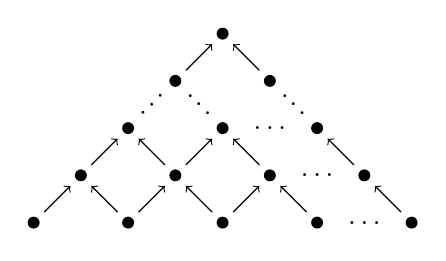
\begin{tikzpicture}[x=0.6cm,y=0.6cm,line cap=round]
		\fill (0,0) circle (0.5ex) coordinate (00);
		\fill (2,0) circle (0.5ex) coordinate (01);
		\fill (4,0) circle (0.5ex) coordinate (02);
		\fill (6,0) circle (0.5ex) coordinate (03);
		\fill (8,0) circle (0.5ex) coordinate (04);
		\fill (1,1) circle (0.5ex) coordinate (10);
		\fill (3,1) circle (0.5ex) coordinate (11);
		\fill (5,1) circle (0.5ex) coordinate (12);
		\fill (7,1) circle (0.5ex) coordinate (13);
		\fill (2,2) circle (0.5ex) coordinate (20);
		\fill (4,2) circle (0.5ex) coordinate (21);
		\fill (6,2) circle (0.5ex) coordinate (22);
		\fill (3,3) circle (0.5ex) coordinate (30);
		\fill (5,3) circle (0.5ex) coordinate (31);
		\fill (4,4) circle (0.5ex) coordinate (40);
		\draw[-to,shorten <=1.25ex,shorten >=1.25ex] (00) -- (10);
		\draw[-to,shorten <=1.25ex,shorten >=1.25ex] (01) -- (10);
		\draw[-to,shorten <=1.25ex,shorten >=1.25ex] (01) -- (11);
		\draw[-to,shorten <=1.25ex,shorten >=1.25ex] (02) -- (11);
		\draw[-to,shorten <=1.25ex,shorten >=1.25ex] (02) -- (12);
		\draw[-to,shorten <=1.25ex,shorten >=1.25ex] (03) -- (12);
		\draw[-to,shorten <=1.25ex,shorten >=1.25ex] (04) -- (13);
		\draw[-to,shorten <=1.25ex,shorten >=1.25ex] (10) -- (20);
		\draw[-to,shorten <=1.25ex,shorten >=1.25ex] (11) -- (20);
		\draw[-to,shorten <=1.25ex,shorten >=1.25ex] (11) -- (21);
		\draw[-to,shorten <=1.25ex,shorten >=1.25ex] (13) -- (22);
		\draw[-to,shorten <=1.25ex,shorten >=1.25ex] (12) -- (21);
		\draw[-to,shorten <=1.25ex,shorten >=1.25ex] (30) -- (40);
		\draw[-to,shorten <=1.25ex,shorten >=1.25ex] (31) -- (40);
		\path (03) to  node[pos=0.5] {$\ldots$} (04);
		\path (12) to  node[pos=0.5] {$\ldots$} (13);
		\path (21) to  node[pos=0.5] {$\ldots$} (22);
		\path (31) to  node[pos=0.5,sloped] {$\ldots$} (22);
		\path (20) to  node[pos=0.5,sloped] {$\ldots$} (30);
		\path (21) to  node[pos=0.5,sloped] {$\ldots$} (30);
	\end{tikzpicture}
\end{center}
And voilà, plenty of spans!
 The corresponding picture for $\Ar(\Delta^n)$ is instead the following:
\begin{center}
	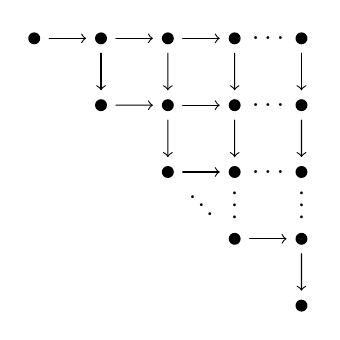
\begin{tikzpicture}[x=0.6cm,y=0.6cm,line cap=round,rotate=-45]
		\fill (0,0) circle (0.5ex) coordinate (00);
		\fill (2,0) circle (0.5ex) coordinate (01);
		\fill (4,0) circle (0.5ex) coordinate (02);
		\fill (6,0) circle (0.5ex) coordinate (03);
		\fill (8,0) circle (0.5ex) coordinate (04);
		\fill (1,1) circle (0.5ex) coordinate (10);
		\fill (3,1) circle (0.5ex) coordinate (11);
		\fill (5,1) circle (0.5ex) coordinate (12);
		\fill (7,1) circle (0.5ex) coordinate (13);
		\fill (2,2) circle (0.5ex) coordinate (20);
		\fill (4,2) circle (0.5ex) coordinate (21);
		\fill (6,2) circle (0.5ex) coordinate (22);
		\fill (3,3) circle (0.5ex) coordinate (30);
		\fill (5,3) circle (0.5ex) coordinate (31);
		\fill (4,4) circle (0.5ex) coordinate (40);
		\draw[-to,shorten <=1.25ex,shorten >=1.25ex] (00) -- (10);
		\draw[-to,shorten <=1.25ex,shorten >=1.25ex] (10) -- (01);
		\draw[-to,shorten <=1.25ex,shorten >=1.25ex] (01) -- (11);
		\draw[-to,shorten <=1.25ex,shorten >=1.25ex] (11) -- (02);
		\draw[-to,shorten <=1.25ex,shorten >=1.25ex] (02) -- (12);
		\path (12) to node[pos=0.5,sloped,rotate=-45] {$\ldots$} (03);
		\draw[-to,shorten <=1.25ex,shorten >=1.25ex] (13) -- (04);
		\draw[-to,shorten <=1.25ex,shorten >=1.25ex] (10) -- (20);
		\draw[-to,shorten <=1.25ex,shorten >=1.25ex] (20) -- (11);
		\draw[-to,shorten <=1.25ex,shorten >=1.25ex] (11) -- (21);
		\draw[-to,shorten <=1.25ex,shorten >=1.25ex] (31) -- (22);
		\draw[-to,shorten <=1.25ex,shorten >=1.25ex] (21) -- (12);
		\path (30) to node[pos=0.5] {$\ldots$} (40);
		\draw[-to,shorten <=1.25ex,shorten >=1.25ex] (40) -- (31);
		\draw[-to,shorten <=1.25ex,shorten >=1.25ex] (20) to  (30);
		\draw[-to,shorten <=1.25ex,shorten >=1.25ex] (03) to  (13);
		\path (02) to  node[pos=0.5,sloped,rotate=-45] {$\ldots$} (03);
		\path (12) to  node[pos=0.5,sloped,rotate=-45] {$\ldots$} (22);
		\path (21) to  node[pos=0.5,sloped,rotate=-45] {$\ldots$} (31);
		\path (22) to  node[pos=0.5,sloped,rotate=-45] {$\ldots$} (13);
		\draw[to-,shorten <=1.25ex,shorten >=1.25ex] (21) to (30);
	\end{tikzpicture}
\end{center}
As a bit of foreshadowing, Fabian mentioned that the first picture is related to the \emph{Quillen $Q$-construction} (see~\cref{par:QuillenQConstruction}), whereas the second is related to the \emph{Segal $S$-construction} (see \cref{con:SConstruction}), which people keep calling \emph{Waldhausen} $S$-construction, even though Waldhausen himself wrote \emph{Segal} $S$-construction.
\begin{exc}\label{exc:coreTwAr=coreAr}
	Show that $\core\TwAr(\Cc)\simeq\core\Ar(\Cc)$ holds for all $\infty$-categories $\Cc$.
\end{exc}
\begin{proof}[Proof sketch]
	See \cite[Proposition~I.31]{KTheory} for a rough sketch.
\end{proof}

\section{Yoneda's Lemma, Limits and Colimits in \texorpdfstring{$\infty$}{Infinity}-Categories}
\subsection{Yoneda's Lemma and Adjunctions}
Now that we have a sufficient supply of mutually equivalent definitions of the $\Hom$ functor, the next step is to prove Yoneda's lemma.
\begin{thm}[Yoneda's lemma]\label{thm:Yoneda}
	Let $\Cc$ be an $\infty$-category. Given a functor $F\colon \Cc\morphism\cat{An}$ and an object $x\in \Cc$, the evaluation map
		\begin{equation*}
			\ev_{\id_x}\colon\Nat\big(\Hom_\Cc(x,-),F\big)\isomorphism F(x)
		\end{equation*}
		is an equivalence \embrace{we use $\Nat$ as a shortcut for $\Hom_{\Fun(\Cc,\cat{An})}$}. Morover, adjoining the functor $\Hom_\Cc\colon\Cc^\op\times\Cc\morphism\Fun(\Cc,\cat{An})$ gives fully faithful functors \embrace{\enquote{Yoneda embeddings}}
		\begin{equation*}
			\Yo^\Cc\colon\Cc\morphism\Fun(\Cc^\op,\cat{An})\quad\text{and}\quad \Yo_\Cc\colon\Cc^\op\morphism\Fun(\Cc,\An)\,.
		\end{equation*}
\end{thm}
%Initially, I used $Y$ to denote the Yoneda embeddings, but then people advised me to use $\Yo$ instead, the hiragana symbol for \emph{yo}, which I think makes a lot of sense.
\begin{proof*}[Proof of \cref{thm:Yoneda}]
	See \cite[Corollaries~XI.2 and~XI.4]{HigherCatsII}.
\end{proof*}
\begin{defi}
	For an $\infty$-category $\Cc$ we denote by $\Pp(\Cc)=\Fun(\Cc^\op,\cat{An})$ the \emph{$\infty$-category of presheaves} on $\Cc$.
\end{defi}
Onwards to adjunctions!
\begin{defi}
	Let $R\colon\Dd\morphism\Cc$ be a functor of $\infty$-categories.
	\begin{alphanumerate}
		\item Given objects $y\in \Cc$, $x\in\Dd$, and a morphism $\eta\colon y\morphism Rx$ in $\Cc$, we say \emph{$\eta$ witnesses $x$ as a left-adjoint object to $y$ under $R$} if the composite
		\begin{equation*}
			\Hom_\Dd(x,-)\morphism[R]\Hom_\Cc(Rx,R-)\morphism[\eta^*]\Hom_\Cc(y,R-) 
		\end{equation*}
		is an equivalence of functors $\Dd\morphism \An$ \embrace{which may be tested on objects by \cref{thm:JoyalEquivalence}\itememph{b}}.
		\item An \emph{adjunction} between $R$ and some functor $L\colon \Cc\morphism\Dd$ is an equivalence
		\begin{equation*}
			\Hom_\Dd(L-,-)\simeq\Hom_\Cc(-,R-)
		\end{equation*}
		as functors $\Cc^\op\times\Cc\morphism\An$.
	\end{alphanumerate}
\end{defi}
A simple but still somewhat surprising and incredibly useful consequence of Yoneda's lemma is that to define left-adjoint functors, it suffices to do so on objects (something that is wildly false for arbitrary functors)!
\begin{cor}\label{cor:AdjointsPointwise}
	A functor $R\colon \Dd\morphism\Cc$ of $\infty$-categories admits a left adjoint if and only if every $y\in \Cc$ admits a left-adjoint object under $R$. More generally, if $\Cc_R\subseteq \Cc$ is the full subcategory spanned by those objects $y\in\Cc$ which admit a left-adjoint object, extracting these left-adjoint objects defines a functor
	\begin{equation*}
		L\colon \Cc_R\morphism \Dd\,.
	\end{equation*}
\end{cor}
\begin{proof}
	We repeat the proof given in \cite[Lemma~XI.6]{HigherCatsII}. Via currying, the functor $\Hom_\Cc(-,R-)\colon \Cc^\op\times\Dd\morphism\cat{An}$ corresponds to a functor $H\colon \Cc^\op\morphism\Fun(\Dd,\cat{An})$. When restricted to $\Cc_R^\op$, it lands in the representables, i.e., in the essential image of the Yoneda embedding $\Yo_\Dd\colon \Dd^\op\morphism\Fun(\Dd,\cat{An})$. By \cref{thm:Yoneda}, $\Yo_\Dd$ is fully faithful, hence an equivalence onto its essential image by \cref{thm:JoyalEquivalence}\itememph{a}. Composing $H|_{\Cc_R^\op}$ with an inverse of this equivalence gives a functor $\Cc_R^\op\morphism\Dd^\op$. Taking $(-)^\op$ we get $L\colon \Cc_R\morphism\Dd$ as required.
	
	By construction, $\Yo_\Dd\circ L^\op$ is equivalent to $H|_{\Cc_R^\op}$ in $\Fun(\Cc_R^\op,\Fun(\Dd,\An))$. But this means that $\Hom_\Dd(L-,-)$ and $\Hom_\Cc(-,R-)$ are equivalent in $\Fun(\Cc_R^\op\times\Dd,\An)$. If $\Cc_R=\Cc$, this proves that $L$ is indeed a left adjoint of $R$.
\end{proof}
\begin{exm}\label{exm:MyFirstAdjoints}
	\enquote{My first adjoint pairs of functors}:
	\begin{alphanumerate}
		\item The inclusion $\cat{An}\subseteq \cat{Cat}_\infty$ has both a left adjoint, the functor $|\blank|\colon \cat{Cat}_\infty\morphism\cat{An}$ (which sends an $\infty$-category to its localisation at all its morphisms), and a right adjoint, given by $\core\colon \cat{Cat}_\infty\morphism\cat{An}$. We proved this in \cite[Example~XI.8]{HigherCatsII}. Moreover, the inclusion $\cat{Set}\morphism\cat{An}$ has $\pi_0\colon\cat{An}\morphism\cat{Set}$ as a left adjoint. In pictures,
		\begin{equation*}
			\begin{tikzcd}
				\Set\rar[symbol=\subseteq] & \An\rar[symbol=\subseteq]\lar[dashed,bend right=45,"\pi_0"']  & \Cat_\infty\lar[dashed,bend right=45,"|\blank|"']\lar[dashed,bend left=45,"\core",shorten >=0.75ex]
			\end{tikzcd}
		\end{equation*}
		Of course we should actually write $\N(\Set)$ instead of $\Set$, but from now on we'll frequently abuse notation that way since writing $\N$ all the time will inevitably get on our \dotso \emph{nerves} (sorry).
		\item Let $\Ii$ be any simplicial set (which we think of as a \enquote{diagram shape}) and consider the functor $\const\colon\Cc\morphism\Fun(\Ii,\Cc)$. Given a map $F\colon \Ii\morphism\Cc$, a left-adjoint object to $F$ under $\const$ is called a \emph{colimit} of $F$ and denoted $\colimit_IF$. Similarly, a right-adjoint object is called a \emph{limit} and denoted $\limit_IF$. In particular, one has
		\begin{equation*}
			\Hom_\Cc\left(\colimit_\Ii F,x\right)\simeq\Nat(F,\const x)
		\end{equation*}
		for all objects $x\in \Cc$, and similarly for $\lim_IF$. We will discuss limits and colimits in detail in the next subsection.
	\end{alphanumerate}
\end{exm}
\subsection{First Properties and Examples of (Co)Limits}
First we'll discuss the main existence theorem for limits and colimits in $\infty$-categories. For that matter, recall the notion of \emph{Kan simplicial model categories} from \cite[Digression~IV Definition~G.2]{HigherCatsII}. For a (not necessarily Kan simplicial) model category $A$, we denote by $A^\mathrm{cf}$ its full subcategory of bifibrant objects (Lurie uses the notation $A^\circ$ instead). Also $(-)^\mathrm{c}\colon A\morphism A$ and $(-)^\mathrm{f}\colon A\morphism A$ denote any choice of cofibrant/fibrant replacement functors.
\begin{thm}\label{thm:HomotopyLimits}
	If $A$ is a Kan simplicial model category, then $\N^c(A^\mathrm{cf})$ has all limits and colimits. For a diagram $F\colon \Ii\morphism \N^c(A^\mathrm{cf})$, these are given by
	\begin{equation*}
		\colimit_\Ii F\simeq \Big(\hocolimit_{\CC[\Ii ]}\snake{F}\Big)^\mathrm{f}\quad\text{and}\quad\limit_\Ii F\simeq\Big(\holimit_{\CC[\Ii]}\snake{F}\Big)^\mathrm{c}\,,
	\end{equation*}
	where $\snake{F}\colon \CC[\Ii]\morphism A^\mathrm{cf}$ is adjoint to $F\colon \Ii\morphism\N^c(A^\mathrm{cf})$.
\end{thm}
\begin{proof*}
	See \cite[Theorem~XI.21]{HigherCatsII}.
\end{proof*}
\begin{rem*}
We'll soon talk about cofinal and final maps (see \cref{def:cofinal} or \cite[\S4.1]{HTT}), but let me already mention that the theory of these allows us to assume that all diagram shapes $\Ii$ are $\infty$-categories. This hardly ever matters, but we formulated \cref{thm:StraighteningCat} for $\infty$-categories only, so I sleep better knowing that $\Ii$ can be chosen that way.
\end{rem*}
\begin{exm}
	Applying \cref{thm:HomotopyLimits} to $A=\sSet$ with its Kan--Quillen model structure or $A=\sSet^+$ (the category of marked simplicial sets) with its marked Joyal model structure, which are Kan simplicial model categories by \cite[Digression~IV Examples~G.3]{HigherCatsII}, shows that $\An$ and $\Cat_\infty$ are complete and cocomplete (i.e.\ have all limits and colimits).
	
	Another example of a complete and cocomplete $\infty$-category is $\Kk(R)$ for any ring $R$, as defined in \cref{exm:MyFirstInftyCats}\itememph{e}. In this case though, we can't apply \cref{thm:HomotopyLimits}, since $\Kk(R)$ is (probably) not given by a Kan simplicial model structure on $\Ch(R)$, at least not for the projective or injective model structure (these have quasi-isomorphisms as weak equivalences, whereas $\Kk(R)$ wants homotopy equivalences). Instead, one has to use some more properties of limits and colimits, which we will develop until \cref{exc:K(R)cocomplete}.
\end{exm}
\begin{exm*}\label{exm*:HomotopyPullbacks}
	Per Bastiaan's suggestion, we give two more examples. Recall that a pullback on the nose in a model category is also a homotopy pullback if all objects are fibrant and one of its legs is a fibration (this follows from Reedy's lemma for example, see \cite[Corollary~VIII.52]{HigherCatsII}). 
	\begin{alphanumerate}
		\item Combining this observation with \cref{thm:HomotopyLimits} shows that the pullback defining $\Hom_\Cc(a,b)$ from \cref{def:Hom} is also a pullback in $\Cat_\infty$, because its vertical leg $\Fun(\Delta^1,\Cc)\morphism\Fun(\partial\Delta^1,\Cc)\simeq \Cc\times\Cc$ is an isofibration (by \cite[Corollary~VII.11]{HigherCatsI}), hence a fibration in the Joyal model structure on $\sSet$.
		\item Likewise, the pullback defining $\Un(F)$ in \cref{thm:StraighteningAn} is a pullback in $\Cat_\infty$, because $*/\An\morphism\An$ is a left fibration, hence an isofibration.
	\end{alphanumerate}
\end{exm*}
For a cocartesian fibration $p\colon E\morphism S$, we denote by $\Gamma(p)$ its \emph{$\infty$-category of sections} defined by the pullback
\begin{equation*}
	\begin{tikzcd}
		\Gamma(p)\rar\dar\drar[pullback] & \Fun(S,E)\dar["p_*"]\\
		\{\id_S\}\rar& \Fun(S,S)
	\end{tikzcd}
\end{equation*}
If we use the new notion from \cref{def:WeirdCocartesianDefinition}\itememph{b} and $p$ is not necessarily an isofibration, we need to take this pullback in $\Cat_\infty$, otherwise it can also be taken in $\sSet$ by the arguments from \cref{exm*:HomotopyPullbacks} above. We let $\Gamma_\cocart(p)\subseteq \Gamma(p)$ denote the full sub-$\infty$-category spanned by sections that take all edges in $S$ to $p$-cocartesian edges.
\begin{prop}[Lurie]\label{prop:CoLimitsInCat}
	Given a diagram $F\colon \Ii\morphism\cat{Cat}_\infty$, we have
	\begin{align*}
		\colimit_\Ii F&\simeq \Un^\cocart(F)\left[\{\text{\upshape cocartesian edges}\}^{-1}\right]\,,\\
		\limit_\Ii F&\simeq \Gamma_\cocart\big(\Un^\cocart(F)\big)\,.
	\end{align*}
	In particular, if $F\colon \Ii\morphism\cat{An}$ takes values in anima, then
	\begin{equation*}
		\colimit_\Ii F\simeq\big|\Un(F)\big|\quad\text{and}\quad\limit_\Ii F\simeq\Gamma\big(\Un(F)\big)\,.
	\end{equation*}
\end{prop}
\begin{proof}[Proof sketch]
	In \cite[Theorem~XI.23]{HigherCatsII} Fabian gave a proof that's basically the same as what we are going to do now, but more on the model category side (but also less sketchy). We only do the case of limits. Consider the diagram
	\begin{equation*}
		\begin{tikzcd}[row sep=small]
			& \Fun(\Ii,\Cat_\infty)\ar[<-,dd,iso,"\St"']\\
			\Cat_\infty\urar["\const",sloped]\drar& \\
			& \Cocart(\Ii)
		\end{tikzcd}
	\end{equation*}
	in which the bottom arrow sends $\Cc\in\Cat_\infty$ to the cocartesian fibration $\pr_2\colon \Cc\times \Ii\morphism \Ii$ over $\Ii$. Let $p\colon E\morphism \Ii$ denote the cocartesian unstraightening of $F$. If $X\simeq\limit_\Ii F$, then we must have equivalences $\Nat(\const\Cc,F)\simeq \Hom_{\Cat_\infty}(\Cc,X)$ for all $\infty$-categories $\Cc$. Applying \cref{thm:StraighteningCat}, this translates into
	\begin{equation*}
		\Hom_{\Cocart(\Ii)}\big((\pr_2\colon \Cc\times \Ii\rightarrow \Ii),(p\colon E\rightarrow \Ii)\big)\simeq \Hom_{\Cat_\infty}(\Cc,X)\,,
	\end{equation*}
	which we'll prove now is fulfilled for $X\simeq\Gamma_\cocart(p)$ (or rather we give an idea why it holds). A map $\phi\colon \Cc\times \Ii\morphism E$ corresponds to a map $\roof{\phi}\colon \Cc\morphism\Fun(\Ii,E)$ via currying. By inspection, $\phi$ commutes with the projection down to $\Ii$ iff $\roof{\phi}$ factors over $\Gamma(p)\morphism E$. Since $\pr_2$-cocartesian edges are precisely those of the form $(\text{equivalence in }\Cc,\text{arbitrary morphism in }\Ii)$, we see that $\phi$ preserves cocartesian edges iff $\roof{\phi}$ sends equivalences $f\colon c\morphism c'$ in $\Cc$ to natural transformations $\eta\colon \roof{\phi}(c)\Rightarrow\roof{\phi}(c')\in\Fun(\Ii,E)_1$ such that for all edges $g\colon i\morphism i'$ in $\Ii$ the composition (or some choice of it)
	\begin{equation*}
		\roof{\phi}(c)(i)\morphism[\eta_i]\roof{\phi}(c')(i)\morphism[g_*]\roof{\phi}(c')(i')
	\end{equation*}
	is $p$-cocartesian in $E$. Since $f\colon c\morphism c'$ is an equivalence in $\Cc$, we get that $\eta_i$ is an equivalence in the fibre $E\times_\Ii\{i\}$ (even in $E$), hence automatically $p$-cocartesian by \cite[Corollary~IX.8]{HigherCatsII}. Thus the composition is $p$-cocartesian iff $g_*$ is $p$-cocartesian, in other words, if $\roof{\phi}(c')$ sends all morphisms in $\Ii$ to $p$-cocartesian edges. Since this holds for all $c'\in \Cc$ (we can always take $f=\id_{c'}$), we finally obtain that $\phi$ preserves $\pr_2$-cocartesian edges iff $\roof{\phi}\colon \Cc\morphism\Gamma(p)$ factors over $\Gamma_\cocart(p)$. \enquote{Thus} $X\simeq \Gamma_\cocart(p)$. 
	
	So far, this is no proof at all, since we only explained why $0$-simplices of $\Nat(\const \Cc,F)$ correspond to $0$-simplices of $\Hom_{\Cat_\infty}(\Cc,\Gamma_\cocart(p))$ but it's not clear how to proceed for higher simplices, nor how to make this an $\infty$-natural transformation. To fix this, first note that we have a map of cocartesian fibrations
	\begin{equation*}
		\begin{tikzcd}
			\Gamma_\cocart(p)\times \Ii\dar["\pr_2"']\rar& E\dar["p"]\\
			\Ii\eqar[r]&\Ii
		\end{tikzcd}
	\end{equation*}
	induced by the evaluation map $\Fun(\Ii,E)\times \Ii\morphism E$. After straightening, this gives a natural transformation $\eta\colon \const\Gamma_\cocart(p)\Rightarrow F$, hence we get
	\begin{equation*}
		\Hom_{\Cat_\infty}\big(-,\Gamma_\cocart(p)\big)\xRightarrow{\const *}\Nat\big(\const-,\const\Gamma_\cocart(p)\big)\overset{\eta_*}{\Longrightarrow}\Nat(\const-,F)\,,
	\end{equation*}
	which is the desired natural transformation. Whether this is an equivalence can be checked pointwise. Since instead of $\Nat(\const-,F)$ we can take the corresponding $\Hom$ anima in $\Cocart(\Ii)$, we arrive at the equivalence from the beginning of the proof. Since we know how to compute $\Hom$ spaces in $\Cat_\infty$ and in $\Cat_\infty/\Ii$ (the latter by \cite[Corollary~VIII.6]{HigherCatsII}), one easily checks $\Hom_{\Cat_\infty}(\Cc,\Gamma(p))\simeq\Hom_{\Cat_\infty/\Ii}((\pr_2\colon\Cc\times \Ii\morphism \Ii),(p\colon E\morphism \Ii))$. Now the $\Hom$ anima we are interested in are full subanima of these, so it really suffices to check that their $0$-simplices correspond, which we did above.
\end{proof}
\begin{exm}\lecture[Localisations. More properties of (co)limits. Left Kan extensions for presheaf categories. $\Hom$ anima in functor categories.]{2020-11-10}\label{exm:Localisation}
	Since $\core\colon\Cat_\infty\morphism\An$ is right-adjoint to the inclusion $\An\subseteq\Cat_\infty$ (\cref{exm:MyFirstAdjoints}\itememph{a}), we get a natural counit transformation $\core\Rightarrow\id_{\Cat_\infty}$, which is given by a map $\Delta^1\morphism\Fun(\Cat_\infty,\Cat_\infty)$. By currying, this yields a functor
	\begin{align*}
		\Cat_\infty&\morphism\Ar(\Cat_\infty)\\
		\Cc&\longmapsto(\core\Cc\rightarrow\Cc)\,.
	\end{align*}
	If $F\colon W\morphism\Cc$ is an object in $\Ar(\Cat_\infty)$, a left-adjoint object to $F$ under the above functor is called a \emph{localisation} of $\Cc$ at $F$ (or rather at the image of $\pi_0\core\Ar(W)\morphism\pi_0\core\Ar(\Cc)$) of $F$ and denoted $\Cc[W^{-1}]$. Unwinding, this means that
	\begin{equation*}
		\Hom_{\Cat_\infty}\big(\Cc[W^{-1}],\Dd\big)\subseteq \Hom_{\Cat_\infty}(\Cc,\Dd)
	\end{equation*}
	is a collection of path components, given by those $G\colon \Cc\morphism\Dd$ such that the composite $G\circ F\colon W\morphism\Dd$ lands in $\core \Dd$. The localisation $\Cc[W^{-1}]$ always exists, as one can take
	\begin{equation*}
		\begin{tikzcd}
			W\rar["F"]\dar\drar[pushout] & \Cc\dar["p"]\\
			{|W|}\rar& \Cc[W^{-1}]
		\end{tikzcd}
	\end{equation*}
	(the pushout is taken in $\Cat_\infty$ of course). Futhermore, it turns out that
	\begin{equation*}
		p^*\colon \Fun\big(\Cc[W^{-1}],\Dd\big)\morphism\Fun(\Cc,\Dd)
	\end{equation*}
	is fully faithful, with essential image spanned by the same functors $G\colon \Cc\morphism\Dd$ as above (see \cite[Proposition~VIII.7]{HigherCatsII} for a proof). This has the funny consequence that the Yoneda embedding induces fully faithful inclusions $\Cc[W^{-1}]\subseteq \Pp\big(\Cc[W^{-1}]\big)\subseteq \Pp(\Cc)$.
	In other words, all localisations of $\Cc$ occur as full subcategories of $\Pp(\Cc)$, which puts a size bound on how large $\Cc[W^{-1}]$ can be.
\end{exm}
\numpar*{Warning \smash{\Attention}}
Localisations are difficult! Localisations of locally small $\infty$-categories may not be locally small any more. Moreover, the localisation of a $1$-category may not be a $1$-category any more.
\begin{exm}\label{exm:Delta0Pushout}
	Let's compute the pushout
	\begin{equation*}
		\begin{tikzcd}
			\Delta^0\rar["1"]\drar[pushout]\dar["0"']& \Delta^1\dar[dashed]\\
			\Delta^1\rar[dashed]& \boldsymbol{?}
		\end{tikzcd}
	\end{equation*}
	in $\Cat_\infty$. One way to do this would be to notice that $0\colon \Delta^0\morphism\Delta^1$ is a cofibration in the Joyal model structure on $\sSet$ (and so is $1\colon \Delta^0\morphism\Delta^1$, but we don't even need this) and all objects are cofibrant, hence the pushout on the nose, which is the $2$-spine $I^2$, is also a homotopy pushout. Now $I^2\subseteq\Delta^2$ is inner anodyne, hence $\Delta^2$ is a fibrant replacement of $I^2$ in the Joyal model structure, which shows that $\boldsymbol{?}\simeq \Delta^2$ is really the pushout in question by \cref{thm:HomotopyLimits}.
	
	 For educational purposes, Fabian presented a less efficient way to show $\boldsymbol{?}\simeq \Delta^2$ using \cref{prop:CoLimitsInCat}. Consider the pushout diagram above as a map $F\colon\Lambda_0^2\morphism\Cat_\infty$. Since all maps in the diagram are nerves of functors of $1$-categories, the cocartesian unstraightening $\Dd=\Un^\cocart(F)$ is simply given by the Grothendieck construction. Therefore, the cocartesian fibration $\Dd\morphism \Lambda_0^2$ can be pictured as follows:
	\begin{center}
		\begin{tikzpicture}[x=0.6cm,y=0.6cm,line cap=round, line join=round]
			\fill (0,0) circle (0.5ex) coordinate (A);
			\fill (-2,0) circle (0.5ex) coordinate (B);
			\fill (-2,1.5) circle (0.5ex) coordinate (C);
			\fill (2,0) circle (0.5ex) coordinate (D);
			\fill (2,1.5) circle (0.5ex) coordinate (E);
			\fill (0,-2.5) circle (0.5ex) coordinate (F);
			\fill (-2,-2.5) circle (0.5ex) coordinate (G);
			\fill (2,-2.5) circle (0.5ex) coordinate (H);
			\node at (-1.4,0.45) {$\scriptscriptstyle /\!/\!/$};
			\draw[dotted, rounded corners=2] (-1.2cm-1ex,0.9cm-1ex) -- (-1ex,-1ex) -- (1.2cm+1ex,-1ex) -- (1.2cm+1ex,0.9cm+1ex) -- (-1.2cm-1ex,0.9cm+1ex) -- cycle;
			\draw[-to,shorten <=1.25ex,shorten >=1.25ex,FabiansPink] (A) to (B);
			\draw[-to,shorten <=1.25ex,shorten >=1.25ex,FabiansPurple!67!FabiansPink] (B) to (C);
			\draw[-to,shorten <=1.25ex,shorten >=1.25ex] (A) to (C);
			\draw[-to,shorten <=1.25ex,shorten >=1.25ex,FabiansPink] (A) to (E);
			\draw[-to,shorten <=1.25ex,shorten >=1.25ex] (D) to (E);
			\draw[-to,shorten <=1.25ex,shorten >=1.25ex] (F) to (G);
			\draw[-to,shorten <=1.25ex,shorten >=1.25ex] (F) to (H);
			\draw[|-to] (0,-0.75cm+0.5\morphismlength) to ++(0,-\the\morphismlength);
			\node at (-3,-2.5) {$\Lambda_0^2$};
			\node at (-3,0.75) {$\Dd$};
			\node at (3,0.75) {$\Dd'$};
		\end{tikzpicture}
	\end{center}
	The two pink edges are the cocartesian ones and thus sent to equivalences in the localisation $\Dd[\{\text{cocartesian edges}\}^{-1}]=\Dd[\{\text{pink edges}\}^{-1}]$. Let $\Dd'$ be the $\infty$-category obtained from $\Dd$ by removing the purple and the pink edge on the left, together with the $2$-simplex spanned by them. We claim that the restriction
	\begin{equation*}
		\Fun^{\{\text{pink}\}}(\Dd,\Ee)\isomorphism \Fun^{\{\text{pink}\}}(\Dd',\Ee)
	\end{equation*}
	is an equivalence for any $\infty$-category $\Ee$, where $\Fun^{\{\text{pink}\}}$ denotes functors that send pink edges to equivalences. Indeed, the purple edge on the left is \enquote{superfluous data}, i.e., any map $\Dd\smallsetminus\{\text{purple edge}\}\morphism\Ee$ has a contractible space of lifts to $\Dd$, by Joyal's lifting theorem. Moreover any map $\Dd'\morphism\Ee$ has a contractible space of lifts to a map $\Dd\smallsetminus\{\text{purple edge}\}\morphism\Ee$ that sends the left pink edge to an equivalence. This proves the above equivalence.
	
	A similar argument shows that it doesn't matter whether we send the pink edge on the right to an equivalence or to an actual identity in $\Ee$. Thus
	\begin{equation*}
		\Fun^{\{\text{pink}\}}(\Dd',\Ee)\simeq\Fun(\Lambda_1^2,\Ee)\simeq\Fun(\Delta^2,\Ee)\,,
	\end{equation*}
	which proves that $\Dd[\{\text{cocartesian edges}\}^{-1}]\simeq\Delta^2$, as claimed.
\end{exm}
\begin{lem}\label{lem:f^*preservesColimits}
	If $\Cc$ is complete or cocomplete, then so is $\Fun(\Dd,\Cc)$ for any $\Dd$. Furthermore, for any $f\colon \Ee\morphism\Dd$, the precomposition functor
	\begin{equation*}
		f^*\colon \Fun(\Dd,\Cc)\morphism\Fun(\Ee,\Cc)
	\end{equation*}
	preserves limits and colimits. In particular \embrace{taking $f$ to be $\{d\}\monomorphism\Dd$ for any $d\in \Dd$}, limits and colimits in functor categories are computed pointwise.
\end{lem}
For the proof we need the following observation.
\begin{obs}\label{obs:AdjunctionOfFunctorCats}
	If $L\colon \Cc \shortdoublelrmorphism \Dd\noloc R$ are adjoint functors, then so are
	\begin{equation*}
		L_*\colon\Fun(\Ee,\Cc)\doublelrmorphism \Fun(\Ee,\Dd)\noloc R_*\quad\text{and}\quad
		R^*\colon\Fun(\Dd,\Ee)\doublelrmorphism \Fun(\Cc,\Ee)\noloc L^*
	\end{equation*}
for any $\infty$-category $\Ee$.
\end{obs}
\begin{proof}
	Being adjoints can be characterized by the existence of a unit and a counit transformation satisfying the triangle identities (see \cite[Proposition~XI.14]{HigherCatsII}, and $L_*$, $R_*$ inherit these transformations from $L$, $R$. Same for $R^*$, $L^*$.
\end{proof}
\begin{obs}\label{obs:AdjointsPreserveLimits}
	Left-adjoint functors preserve colimits, right-adjoint functors preserve limits.
\end{obs}
\begin{proof}
	Straightforward calculation using \cref{obs:AdjunctionOfFunctorCats}. See \cite[Lemma~XI.22]{HigherCatsII} for details.
\end{proof}
\begin{proof}[Proof of \cref{lem:f^*preservesColimits}]
	For any diagram shape $\Ii$, consider the commutative diagram
	\begin{equation*}
		\begin{tikzcd}[row sep=small]
			& \Fun\big(\Ii,\Fun(\Dd,\Cc)\big)\eqar[dd]\\
			\Fun(\Dd,\Cc)\urar["\const",sloped]\drar["\const *"', sloped]& \\
			& \Fun\big(\Dd,\Fun(\Ii,\Cc)\big)\ular[dotted, bend right,"\colimit_*"', end anchor=east,start anchor=160,shorten <=2ex]\ular[dotted, bend left,"\limit_*",start anchor=west, end anchor=330]
		\end{tikzcd}
	\end{equation*}
	By \cref{obs:AdjunctionOfFunctorCats}, $\colimit_*$ and $\limit_*$ are left and right adjoints of $\const *$ respectively, which proves that $\const\colon \Fun(\Dd,\Cc)\morphism \Fun(\Ii,\Fun(\Dd,\Cc))$ has a left and right adjoint as well. Hence $\Fun(\Dd,\Cc)$ is complete and cocomplete again. Moreover, the assertion that limits and colimits are computed pointwise follows by unraveling.
	
	It remains to show that $f^*\colon \Fun(\Dd,\Cc)\morphism\Fun(\Ee,\Cc)$ preserves limits and colimits. For any diagram $F\colon \Ii\morphism\Fun(\Dd,\Cc)$ we get a map
	\begin{equation*}
		\colimit_\Ii f^*F\morphism f^*\colimit_\Ii F
	\end{equation*}
	(unique up to contractible choice). Whether this is an equivalence in $\Fun(\Ee,\Cc)$ can be checked pointwise (by \cref{thm:JoyalEquivalence}\itememph{b}), i.e., after composition with $x^*\colon \Fun(\Ee,\Cc)\morphism\Fun(\{x\},\Cc)\simeq \Cc$ for all $x\in \Ee$. Since we already know that colimits in $\Fun(\Ee,\Cc)$ and $\Fun(\Dd,\Cc)$ are computed pointwise, we see that both $x^*\colimit_\Ii f^*F$ and $x^*f^*\colimit_\Ii F$ are colimits of the diagram $\Ii\times\{f(x)\}\morphism \Cc$ induced by currying of $F$ and restriction along $\{f(x)\}\monomorphism\Dd$.
\end{proof}
\begin{prop}\label{prop:ColimitsCommute}
	Let $p\colon \Ee\morphism\Cc$ be a cocartesian fibration and $F\colon \Ee\morphism\Dd$ a diagram. Suppose that the restrictions $F_{|c}\colon\Ee_{|c}\morphism\Dd$ of $F$ to the fibres $\Ee_{|c}=\Ee\times_\Cc\{c\}$ of $p$ have colimits for all $c\in \Cc$. Then these assemble into a functor $G\colon \Cc\morphism\Dd$ sending $c\mapsto \colimit_{\Ee_{|c}}F_{|c}$, and
	\begin{equation*}
		\colimit_\Ee F\simeq \colimit_\Cc G\,,
	\end{equation*}
	whenever either exists. In particular \embrace{taking $p$ to be the projection $\pr_2\colon \Ii\times\Cc\morphism\Cc$ for some $\infty$-category $\Ii$}, this means that \enquote{colimits commute}. Also a dual assertion holds, with $p$ a cartesian fibration and all colimits replaced by limits.
\end{prop}
\begin{proof*}
	Fabian claims (I think) this follows from \cite[Proposition~\HTTthm{4.3.2.12}]{HTT}, but Lurie's proof is rather laborious, so I'll give my own proof*. As it turns out, the arguments are pretty much the same as for the proof of Theorems~\labelcref{thm:ColimitPreservingRepresentable,thm:KanExtension} in Fabians notes. I'll freely reference later results (without running into circular arguments, I hope).
	
	We won't prove the assertion as stated above, but its dualized version. The reason is that the direct proof of the undualized version is quite confusing (for example, neither of the Yoneda embeddings preserves colimits, so we would have to consider $(\Yo^\Dd)^\op\colon \Dd^\op\morphism\Pp(\Dd)^\op$) and it seems cleaner to prove the dualized statement and then deduce the undualized one by applying the dual statement to $p^\op\colon \Ee^\op\morphism\Cc^\op$.
	
	So let $p\colon \Ee\morphism\Cc$ be cartesian instead. We want to construct $G$ as the right Kan extension $G\simeq p_*F$. Let's first consider the case where $\Dd$ is replaced by $\Pp(\Dd)$. Then the dual of \cref{thm:StraighteningAn} implies $\Fun(\Cc,\Pp(\Dd))\simeq \Fun(\Cc\times\Dd^\op,\An)\simeq \Right(\Cc^\op\times\Dd)$ and same for $\Ee$, so we may apply \cref{lem*:SmoothBaseChange} below to the cocartesian fibration $p^\op\times\id_\Dd\colon \Ee^\op\times\Dd\morphism\Cc^\op\times\Dd$ to see that $p^*\colon \Fun(\Cc,\Pp(\Dd))\morphism\Fun(\Ee,\Pp(\Dd))$ has a right adjoint $p_*$. Now consider the diagram
	\begin{equation*}
		\begin{tikzcd}
			\Fun\big(\Cc,\Pp(\Dd)\big)\rar["p^*"]\dar["c^*"']& \Fun\big(\Ee,\Pp(\Dd)\big)\dar["i^*"]\\
			\Fun\big(\{c\},\Pp(\Dd)\big)\rar["p_{|c}^*"]& \Fun\big(\Ee_{|c},\Pp(\Dd)\big)
		\end{tikzcd}
	\end{equation*}
	where $i\colon \Ee_{|c}\monomorphism \Ee$ denotes the inclusion of the fibre. The second part of \cref{lem*:SmoothBaseChange} ensures that $c^*p_*F\simeq p_{|c,*}i^*F$. By inspection, right Kan extension along the functor $p_{|c}\colon \Ee_{|c}\morphism\{c\}$ is given by taking a functor $G\colon \Ee_{|c}\morphism\Pp(\Dd)$ to $\limit_{\Ee_{|c}}G$. This implies $p_*F(c)\simeq \limit_{\Ee_{|c}}F_{|c}$, so $p_*F$ takes the correct values. Moreover, limits over $\Cc$ are given by right Kan extension along the unique map $\pi\colon \Cc\morphism *$, and similar for $\pi\circ p\colon \Ee\morphism *$, hence
	\begin{equation*}
		\limit_\Cc p_*F\simeq \pi_*p_*F\simeq (\pi\circ p)_*F\simeq \limit_\Ee F
	\end{equation*}
	since right adjoints compose. This finishes the proof for $\Pp(\Dd)$.
	
	Now for the case of general $\Dd$. The Yoneda embedding $\Yo^\Dd\colon \Dd\morphism\Pp(\Dd)$ is fully faithful, hence an equivalence onto its essential image. To obtain a functor $p_*F\colon \Cc\morphism\Dd$, it thus suffices to check that $p_*(\Yo^\Dd\circ F)\colon \Cc\morphism\Pp(\Dd)$ has image in the representable functors. By assumption, all limits $\limit_{\Ee_{|c}}F_{|c}$ exist in $\Dd$ and $\Yo^\Dd$ preserves limits by \cref{cor:HomPreservesColimits}, hence the description of the values $p_*(Y\circ F)(c)$ for $c\in \Cc$ shows that indeed it takes values in the representables. Thus $p_*F\colon \Cc\morphism\Dd$ exists. The additional assertion about limits follows as above, noting that the limits in question exist in $\Dd$ if and only if the limits taken in $\Pp(\Dd)$ (where they definitely exist) are representable, since $\Yo^\Dd$ is fully faithful and preserves limits.
\end{proof*}
\begin{lem*}\label{lem*:SmoothBaseChange}
	Let $p\colon \Cc\morphism\Dd$ be a cocartesian fibration of $\infty$-categories. Consider a pullback square \embrace{inside $\Cat_\infty$} as on the left
	\begin{equation*}
		\begin{tikzcd}
			\Cc'\rar["q"]\dar["g"']\drar[pullback] & \Dd'\vphantom{(}\dar["f"]\\
			\Cc\rar["p"]& \Dd \vphantom{(}
		\end{tikzcd}\quad\longrightsquigarrow{\morphismlength-0.145em}\quad\begin{tikzcd}
		\Right(\Cc')\rar[dotted,bend right,"q_*"]& \Right(\Dd')\lar["q^*"']\\
		\Right(\Cc)\uar["g^*"]\rar[dotted,bend right,"p_*"] & \Right(\Dd)\uar["f^*"']\lar["p^*"']
	\end{tikzcd}
	\end{equation*}
	inducing a square as on the right. Then $p^*$ and $q^*$ have right adjoints $p_*$ and $q_*$ as indicated. Moreover, there's a natural equivalence
	\begin{equation*}
		f^*p_*\overset{\sim}{\Longrightarrow} q_*g^*\,.
	\end{equation*}
\end{lem*}
\begin{proof*}
	Without loss of generality all cartesian or right fibrations can be taken in the old sense. Recall (e.g.\ from the dual of \cite[\S2.1.4]{HTT}) that there exists the \emph{contravariant model structure} on $\sSet/\Cc$, in which the cofibrations are monomorphisms of simplicial sets and fibrant objects are given by right fibrations over $\Cc$ (general fibrations are more complicated). The functor $p^*\colon\sSet/\Dd\morphism\sSet/\Cc$ has a right adjoint $p_*$ for abstract reasons: It's straightforward to check that $p^*$ preserves colimits, so \cref{thm:2Yoneda} can be applied to $\sSet/\Dd\simeq\Pp((\Delta/\Dd)^\op)$ (here $\Delta/S$ denotes the slice category with respect to the functor $\Delta\colon \IDelta\morphism\sSet$ sending $[n]\mapsto \Delta^n$). We claim that
	\begin{equation*}
		p^*\colon \sSet/\Dd\doublelrmorphism\sSet/\Cc\noloc p_*
	\end{equation*}
	is even a Quillen adjunction when $p$ is a cocartesian fibration. Indeed, it's clear that $p^*$ preserves cofibrations and cofibrant objects. For preservation of trivial cofibrations, we refer to \cite[Proposition~\HTTthm{4.1.2.15}]{HTT} or the dual of \cite[Proposition~X.43]{HigherCatsII} for the essential case.
	
	As for any Quillen adjunction of model categories, we get an induced adjunction
	\begin{equation*}
		Lp^*\colon (\sSet/\Cc)_\infty\doublelrmorphism(\sSet/\Dd)_\infty\noloc Rp_*
	\end{equation*}
	on underlying $\infty$-categories, defined as the localisations at all weak equivalences, or equivalently as $\N^c((\sSet/\Cc)^{\mathrm{cf}})$ and $\N^c((\sSet/\Cc)^{\mathrm{cf}})$, since $\sSet/\Cc$ and $\sSet/\Dd$ can be made into a Kan simplicial model categories, so \cite[Digression~III Theorem~D]{HigherCatsII} applies. The latter description shows that the underlying $\infty$-categories identify with $\Right(\Cc)$ and $\Right(\Dd)$. Hence $Lp^*$ (which we abbreviate to $p^*$ in the following) has indeed an adjoint $Rp_*$ (which we abbreviate to $p_*$).
	
	So $p_*$ and $q_*$ exist. The counit $p^*p_*\Rightarrow \id$ induces a transformation $q^*f^*p_*\simeq g^*p^*p_*\Rightarrow g^*$, whose adjoint is the transformation $f^*p_*\Rightarrow q_*g^*$. Whether this is an equivalence can be checked on objects. However, explicitly computing $p_*$ and $q_*$ is nasty, so we employ a trick: By Yoneda, it suffices to check that $\Hom_{\Right(\Dd')}(-,f^*p_*-)\Rightarrow \Hom_{\Right(\Dd')}(-,q_*g^*-)$ is a natural equivalence. But $f^*$ and $g^*$ have left adjoints $f_!$ and $g_!$ by \cref{thm:JoyalRightFibrations}, so we may as well show that $\Hom_{\Right(\Cc)}(p^*f_!-,-)\Rightarrow \Hom_{\Right(\Cc)}(g_!q^*-,-)$ is an equivalence, i.e., that $g_!q^*\Rightarrow p^*f_!$ is an equivalence. This is now easily checked on objects: Unravelling, we need to prove that if $X\epimorphism\Dd'$ is a right fibration and $X\monomorphism Y\epimorphism \Dd$ is a factorisation into a right anodyne and a right fibration, then $X\times_\Dd\Cc\monomorphism Y\times_\Dd\Cc$ is right anodyne again, which follows from the references above since $p\colon \Cc\morphism\Dd$ is cocartesian.
\end{proof*}
\begin{thm}[Joyal's version of Quillen's Theorem A]\label{thm:JoyalQuillenThmA}
	For a functor $\alpha\colon \Ii\morphism \Jj$ the following statements are equivalent.
	\begin{alphanumerate}
		\item A functor $F\colon \Jj\morphism\Cc$ has a colimit iff the composition $F\circ\alpha\colon \Ii\morphism \Cc$ has a colimit, and in this case
		\begin{equation*}
			\colimit_\Ii F\circ\alpha\simeq\colimit_\Jj F\,.
		\end{equation*}
		\item For all $j\in \Jj$ we have $|j/\alpha|\simeq *$, i.e., the slice category $j/\alpha$ is weakly contractible. Here we define $j/\alpha$ by the pullback
		\begin{equation*}
			\begin{tikzcd}[column sep=large]
				j/\alpha\dar \rar\drar[pullback]&\Ar(\Jj)\dar["{(s,t)}"]\\
				\{j\}\times\Ii\rar["{(\operatorname{incl},\alpha)}"]&\Jj\times \Jj
			\end{tikzcd}
		\end{equation*}
		Also observe that $j/\alpha=\Ii\times_\Jj j/\Jj$, which is how people usually denote this in the literature.
	\end{alphanumerate}
\end{thm}
\begin{proof*}
	Combine \cite[Proposition~\HTTthm{4.1.1.8}]{HTT} (for more equivalent characterisations) and \cite[Theorem~\HTTthm{4.1.3.1}]{HTT} (for the actual proof).
\end{proof*}
\begin{defi}\label{def:cofinal}
	Maps $\alpha\colon \Ii\morphism \Jj$ as in \cref{thm:JoyalQuillenThmA} are called \emph{cofinal}. Dually, if precomposition with $\alpha$ preserves limits and detects their existence, then $\alpha$ is called \emph{final}.
\end{defi}
Cofinal maps induce homotopy equivalences $|\alpha|\colon |\Ii|\morphism|\Jj|$ of anima, which can be seen via the chain of homotopy equivalences
\begin{equation*}
	|\Ii|\simeq\colimit_\Ii\const *\simeq\colimit_\Jj\const *\simeq|\Jj|
\end{equation*}
(the colimits in the middle are taken in $\An$). Here we use $|\Ii|\simeq\colimit_\Ii\const *$, which can be seen in several ways: One could use \cref{thm:HomotopyLimits} and the Bousfield--Kan formula (\cite[Digression~III]{HigherCatsII}). Alternatively, compute $\Hom_{\An}(\colimit_\Ii\const *,K)\simeq \limit_\Ii\Hom_{\An}(*,K)\simeq\limit_\Ii K$ for any anima $K$ using \cref{cor:HomPreservesColimits} below, and apply \cref{prop:CoLimitsInCat} to get $\limit_\Ii K\simeq\Gamma(\pr_2\colon K\times \Ii\morphism\Ii)$. The space of sections of $\pr_2\colon K\times\Ii\morphism\Ii$ clearly identifies with $\Fun(\Ii,K)\simeq\core\Fun(\Ii,K)\simeq\Hom_{\Cat_\infty}(\Ii,K)$, so $\colimit_\Ii\const *$ is indeed a left-adjoint object of $\Ii$ under the inclusion $\An\subseteq\Cat_\infty$.

Examples of cofinal maps are given by right-adjoint functors and localisations. Indeed, if $\alpha\colon \Ii\morphism\Jj$ is a right adjoint, then consider the diagram
\begin{equation*}
	\begin{tikzcd}[column sep=small]
		& \Cc\dlar["\const"{sloped}]\drar["\const"{sloped}]& \\
		\Fun(\Jj,\Cc)\ar[rr,"\alpha^*"]\urar[bend left=45, dotted,"\colimit_\Jj"] & & \Fun(\Ii,\Cc)\ular[bend right=45, dotted,"\colimit_\Ii"']
	\end{tikzcd}
\end{equation*}
By \cref{obs:AdjunctionOfFunctorCats}, $\alpha^*\colon \Fun(\Jj,\Cc)\morphism\Fun(\Ii,\Cc)$ is a left-adjoint. Since left-adjoints compose, we obtain $\colimit_\Jj\simeq {\colimit_\Ii}\circ\alpha^*$, as required. If $p\colon \Cc\morphism\Cc[W^{-1}]$ is a localisation and $F\colon \Cc[W^{-1}]\morphism\Dd$ is any diagram, then 
\begin{equation*}
	\Nat(F,\const x)\simeq\Nat(F\circ p,\const x)
\end{equation*}
holds for every $x\in \Cc$ since $p^*\colon \Fun(\Cc[W^{-1}],\Dd)\morphism\Fun(\Cc,\Dd)$ is fully faithful, which again proves cofinality by means of \cref{thm:JoyalQuillenThmA}\itememph{a}.
\begin{cor}\label{cor:ColimitsCommute}
	Let $G\colon \Ii\morphism\Cat_\infty$ be a diagram and put $\Jj\simeq\colimit_\Ii G$. Let $F\colon \Jj\morphism\Dd$ be another diagram and suppose that the restrictions 
	\begin{equation*}
		G(i)\morphism\Jj\morphism[F]\Dd
	\end{equation*}
	have colimits for all $i\in \Ii$. Then these colimits assemble into a functor $H\colon \Ii\morphism \Dd$ sending $i\mapsto \colimit_{G(i)}F$, and we have
	\begin{equation*}
		\colimit_\Jj F\simeq\colimit_\Ii H
	\end{equation*}
	if either exists.
\end{cor}
\begin{proof}
	By \cref{prop:CoLimitsInCat}, we have $\Jj\simeq\colimit_\Ii G\simeq \Un^\cocart(G)[\{\text{cocartesian edges}\}^{-1}]$. Since localisations are cofinal, we obtain
	\begin{equation*}
		\colimit_\Jj F\simeq\colimit_{\Un^{\cocart}(G)}F\,.
	\end{equation*}
	Now recall that $G(i)\simeq \Un^\cocart(G)\times_\Ii\{i\}$, so we are done by \cref{prop:ColimitsCommute}.
\end{proof}
\numpar{\enquote{Corollary}}\label{cor:completeIffPullbacksProducts}\itshape If $\Cc$ has coproducts and pushouts, then it is cocomplete. Dually, if $\Cc$ has products and pullbacks, then it is complete.\upshape
\begin{proof}[\enquote{Proof} sketch]
	Decompose any test category $\Ii$ into its skeleta and repeatedly apply \cref{cor:ColimitsCommute} using $\colimit_{\Delta^n}F=F(n)$ since $\{n\}\monomorphism \Delta^n$ is cofinal---in fact, all right anodyne maps are cofinal. For a complete proof, check out \cite[Proposition~\HTTthm{4.4.2.6}]{HTT}.
\end{proof}
\subsection{Colimits and the Yoneda embedding}
We start with an existence result for \enquote{Kan extensions} which was already used in the proof* of \cref{prop:ColimitsCommute}.
\begin{thm}[Joyal]\label{thm:JoyalRightFibrations}
	Given an arbitrary functor $f\colon \Cc\morphism\Dd$ of $\infty$-categories, the pullback functor 
	\begin{equation*}
		f^*\colon \Right(\Dd)\morphism\Right(\Cc)
	\end{equation*}
	admits a left-adjoint. Its value on $p\colon \Ee\morphism\Cc$ is obtained by factoring $\Ee\morphism\Cc\morphism\Dd$ as a cofinal map followed by a right fibration $p'\colon\Ee'\morphism\Dd$. In diagrams
	\begin{equation*}
		\begin{tikzcd}
			\Ee\dar["p"']\rar& \Ee'\dar["\vphantom{p}\smash{p'}"]\\
			\Cc\rar["f"]&\Dd
		\end{tikzcd}
	\end{equation*}
	where the top arrow is cofinal.
\end{thm}
\begin{proof*}[Proof sketch]
	One way to prove this would be to use the contravariant model structures on $\sSet/\Cc$ and $\sSet/\Dd$ as in the proof* of \cref{lem*:SmoothBaseChange}: One shows that $f^*\colon \sSet/\Dd\morphism\sSet/\Cc$ has a left Quillen adjoint $f_!$, sending $\Ee\morphism\Cc$ to $\Ee\morphism\Cc\morphism\Dd$. Since right anodyne maps are cofinal (\cite[Proposition~\HTTthm{4.1.1.3}]{HTT} or \cite[Theorem~XI.28]{HigherCatsII}), a quick unraveling shows that $Lf_!$ can indeed be described as above.
	
	However, Bastiaan has pointed out a simpler proof that doesn't need any model categories. We will proceed in three steps:
	\begin{numerate}\itshape
		\item The pullback functor $f^*\colon \Cat_\infty/\Dd\morphism\Cat_\infty/\Cc$ \embrace{where we take the pullback along $f$ in $\Cat_\infty$} has a left adjoint. On objects, it is the \enquote{forgetful functor} sending $p\colon \Ee\morphism\Cc$ to $f\circ p\colon \Ee\morphism\Cc\morphism\Dd$.
		\item Under the fully faithful inclusions $\Right(\Cc)\subseteq\Cat_\infty/\Cc$ and $\Right(\Dd)\subseteq\Cat_\infty/\Dd$, the pullback functor $f^*\colon \Cat_\infty/\Dd\morphism\Cat_\infty/\Cc$ restricts to $f^*\colon \Right(\Dd)\morphism\Right(\Cc)$ from the formulation of the theorem.
		\item The fully faithful inclusion $\Right(\Dd)\subseteq\Cat_\infty/\Dd$ has a left adjoint, sending an object $q\colon\Ee\morphism\Dd$ to $q'\colon\Ee'\morphism\Dd$, where $\Ee\morphism\Ee'\morphism\Dd$ is any factorisation into a cofinal map followed by a right fibration.
	\end{numerate}
	
	Since left adjoints compose, combining \itememph{1}, \itememph{2}, and \itememph{3} shows that $f^*\colon \Right(\Dd)\morphism\Right(\Cc)$ has a left adjoint $f_!$ with the desired description on objects.
		
	To show \itememph{1}, we use \cref{cor:AdjointsPointwise} to see that it suffices to show that $f\circ p$ is a left adjoint object of $p$ for any $(p\colon \Ee\morphism\Cc)\in \Cat_\infty/\Cc$. If we had the dual of \cref{cor:HomPreservesColimits} below already, this would be almost trivial, but as it is, we need to be a bit careful. Factor $f\circ p$ into a Joyal equivalence $\Ee\morphism \Ee'$ followed by an isofibration $p'\colon\Ee'\morphism\Dd$. Then $f^*\Ee'$ equals the same pullback taken in $\sSet$ by \cref{thm:HomotopyLimits}. Hence there is a natural map $\Ee\morphism f^*\Ee'$. Together with functoriality of $f^*$, it induces natural transformations
	\begin{align*}
		\Hom_{\Cat_\infty/\Dd}(\Ee,-)\simeq \Hom_{\Cat_\infty/\Dd}(\Ee',-)&\Longrightarrow \Hom_{\Cat_\infty/\Cc}\big(f^*\Ee',f^*(-)\big)\\
		&\Longrightarrow \Hom_{\Cat_\infty/\Cc}\big(\Ee,f^*(-)\big)\,.
	\end{align*}
	We are to show that the composite is an equivalence. By \cref{thm:JoyalEquivalence}\itememph{b}, this can be done on objects. Let $T\morphism\Dd$ be an bject of $\Cat_\infty/\Dd$, which we may choose to be an isofibration without restriction, so that $f^*(T)$ agrees with the corresponding pullback in $\sSet$. Consider $\Fun_\Dd(\Ee,T)\coloneqq\Fun(\Ee,T)\times_{\Fun(\Ee,\Dd)}\{f\circ p\}$ and define $\Fun_\Cc(\Ee,f^*(T))$ similarly. Since $T\morphism\Dd$ is an isofibration, it doesn't matter whether this pullback is taken in $\sSet$ or in $\Cat_\infty$. Moreover, $\core(-)$ transforms pullbacks in $\Cat_\infty$ into pullbacks in $\An$ (it is a right adjoint by \cref{exm:MyFirstAdjoints}\itememph{a}, so \cref{obs:AdjointsPreserveLimits} can be applied), hence our computation of $\Hom$ anima in slice categories from \cite[Corollary~VIII.6]{HigherCatsII} shows $\Hom_{\Cat_\infty/\Dd}(\Ee,T)\simeq \core \Fun_\Dd(\Ee,T)$. Likewise, $\Hom_{\Cat_\infty/\Cc}(\Ee,f^*(T))\simeq \core \Fun_\Cc(\Ee,f^*(T))$. Now the universal property of $f^*(T)$ as a pullback in $\sSet$ implies $\Fun_\Dd(\Ee,T)\simeq \Fun_\Cc(\Ee,f^*(T))$, which proves step~\itememph{1}.
	
	For \itememph{2}, observe that $f^*$ of a right fibration in the old sense can also be taken in $\sSet$ by \cref{thm:HomotopyLimits} again, and right fibrations (in the old sense) are preserved under pullbacks formed in $\sSet$. Hence right fibrations in the new sense are preserved by pullbacks in $\Cat_\infty$.
	
	Finally, to show \itememph{3}, we can argue as \itememph{1} to reduce the assertion to $\Fun_\Dd(\Ee',T)\simeq\Fun_\Dd(\Ee,T)$ for any right fibration $T\morphism\Dd$ and any cofinal map $\Ee'\morphism \Ee$ over $\Dd$. 	But this is precisely how Lurie defines cofinal maps in \cite[Definition~\HTTthm{4.1.1.1}]{HTT}, and his definition is equivalent to our \cref{def:cofinal}.
\end{proof*}
\begin{cor}\label{cor:f_!:PC->PD}
	The functor $f^*\colon \Pp(\Dd)\morphism\Pp(\Cc)$ has a left-adjoint $f_!$ \embrace{given by left Kan extension} such that the diagram
	\begin{equation*}
		\begin{tikzcd}
			\Cc\rar["f"]\dar["\Yo^\Cc"']& \Dd\dar["\Yo^\Dd"]\\			\Pp(\Cc)\rar["f_!"]&\Pp(\Dd)
		\end{tikzcd}
	\end{equation*}
	 commutes in the $\infty$-category $\Cat_\infty$.
\end{cor}
\begin{proof}
	The first statement immediately follows from \cref{thm:JoyalRightFibrations} and (the dual of) \cref{thm:StraighteningAn}, which asserts that the cartesian straightening $\St^\cart\colon \Right(\Cc)\isomorphism\Pp(\Cc)$ is an equivalence with inverse the cartesian unstraightening $\Un^\cart$.
	
	For the second statement, we have to show that $f_!\Hom_\Cc(-,x)\morphism\Hom_\Dd(-,f(x))$ is an equivalence for all $x\in \Cc$.	After unstraightening, this translates to the statement that the diagram
	\begin{equation*}
		\begin{tikzcd}
			\Cc/x\dar\rar& \Dd/f(x)\dar\\
			\Cc\rar["f"]&\Dd
		\end{tikzcd}
	\end{equation*}
	exhibits $\Dd/f(x)\morphism\Dd$ as $f_!(\Cc/x\morphism\Cc)$. The right vertical arrow is already a right fibration, so it suffices to check that $\Cc/x\morphism\Dd/f(x)$ is cofinal. This holds because
	\begin{equation*}
		\begin{tikzcd}[column sep=small]
			& \Delta^0\dlar["x"']\drar["f(x)"] & \\
			\Cc/x\ar[rr,"f"]& & \Dd/f(x)
		\end{tikzcd}
	\end{equation*}
	has both downward arrows cofinal (as $x$ and $f(x)$ are terminal objects in $\Cc/x$ and $\Dd/f(x)$ respectively and thus both sloped arrows are right anodyne by \cite[Digression~I Corollary~D.7]{HigherCatsII}).
\end{proof}
\begin{cor}\label{cor:HomInFunctorCats}
	Given functors $F,G\colon \Cc\morphism\Dd$ of $\infty$-categories, we have an equivalence of anima
	\begin{equation*}
		\Nat(F,G)\simeq\limit_{(x\rightarrow y)\in\TwAr(\Cc)}\Hom_\Dd\big(F(x),G(y)\big)\,.
	\end{equation*}
	Explicitly, the limit is taken over $\TwAr(\Cc)\morphism\Cc^\op\times\Cc\xrightarrow{F^\op\times G}\Dd^\op\times\Dd\xrightarrow{\Hom_\Dd}\An$.
\end{cor}
Note that \cref{cor:HomInFunctorCats} explains why natural transformations are complicated in $\infty$-land: $\pi_0$ does not commute with arbitrary limits!
\begin{proof}[Proof of \cref{cor:HomInFunctorCats}]
	By \cref{prop:CoLimitsInCat}, the right-hand side can be computed as the anima of sections of $p\colon P\morphism\TwAr(\Cc)$, where $P$ denotes the correct unstraightening. Explicitly, we have a diagram
	\begin{equation*}
		\begin{tikzcd}
			P\rar\dar\drar[pullback] & P'\rar\dar\drar[pullback] & \TwAr(\Dd)\dar\rar\drar[pullback] & */\An\dar\\
			\TwAr(\Cc)\rar["{(s,t)}"] & \Cc^\op\morphism\Cc\rar["F^\op\times G"] & \Dd^\op\times\Dd\rar["\Hom_\Dd"] & \An
		\end{tikzcd}
	\end{equation*}
	which shows $\Gamma(p)\simeq\Hom_{\Cat_\infty/\Cc^\op\times\Cc}(\TwAr(\Cc),P')$. But these are both left fibrations over $\Cc^\op\times\Cc$, so the $\Hom$ anima on the right-hand side can be equivalently computed as $\Nat(\Hom_\Cc,{\Hom_\Dd}\circ(F^\op\times G))$. Now the currying equality  $\Fun(\Cc^\op\times\Cc,\An)=\Fun(\Cc,\Pp(\Cc))$ sends $\Hom_\Cc$ to $\Yo^\Cc$ and ${\Hom_\Dd}\circ(F^\op\times G)$ to $F^*\circ \Yo^\Dd\circ G$, hence the $\Hom$ anima under consideration is given by
	\begin{equation*}
		\Nat\big(\Yo^\Cc,F^*\circ \Yo^\Dd\circ G)\big)\simeq \Nat(F_!\circ \Yo^\Cc,\Yo^\Dd\circ G)\simeq \Nat(\Yo^\Dd\circ F,\Yo^\Dd\circ G)\simeq \Nat(F,G)\,,
	\end{equation*}
	as claimed. For the left equivalence, we use that $F_!\circ -$ is an adjoint of $F^*\circ -$ by construction and \cref{obs:AdjunctionOfFunctorCats}, the middle equivalence follows from \cref{cor:f_!:PC->PD}, and the right one since $\Yo^\Dd\colon \Dd\morphism\Pp(\Dd)$ is fully faithful by Yoneda's lemma (\cref{thm:Yoneda}).
\end{proof}
\begin{cor}\label{cor:HomPreservesColimits}
	Let $F\colon \Ii\morphism\Cc$ be a functor of $\infty$-categories. A natural transformation $\eta\colon F\Rightarrow\const c$ exhibits $c\in \Cc$ as the colimit of $F$ if and only if the natural map
	\begin{equation*}
		\eta^*\colon \Hom_\Cc(c,x)\isomorphism\limit_{i\in\Ii^\op}\Hom_\Cc\big(F(i),x\big)
	\end{equation*}
	is an equivalence for all $x\in \Cc$. A similar assertion holds for limits. In particular, the functors $\Hom_\Cc(-,d)\colon \Cc^\op\morphism\An$ and $\Yo^\Cc\colon \Cc\morphism\Pp(\Cc)$ preserve limits.
\end{cor}
\begin{proof}
	We are done if we can show that the right-hand side is just $\Nat(F,\const x)$. From \cref{cor:HomInFunctorCats} we get a map
	\begin{equation*}
		\Nat(F,\const x)\simeq \limit_{(i\rightarrow i')\in\TwAr(\Ii)}\Hom_\Cc(F(i),x)\morphism\limit_{i\in\Ii^\op}\Hom_\Cc(F(i),x)\,.
	\end{equation*}
	So we are done if we show that $s\colon\TwAr(\Ii)\morphism\Ii^\op$ is final. By (the dual of) \cref{thm:JoyalQuillenThmA}\itememph{b} we must show $|s/i|\simeq *$ for all $i\in \Ii^\op$. Applying \cref{exc:cocartesianFibrationLeftAdjoint} to the cocartesian fibration $s={\pr_2}\circ(s,t)\colon\TwAr(\Ii)\morphism\Ii^\op\times\Ii\morphism\Ii^\op$, we find that $|s^{-1}\{i\}|\simeq|s/i|$ since adjoints induce inverse homotopy equivalences after applying $|\blank|$; alternatively one can use that left adjoints are final. Now $s^{-1}\{i\}$ has an initial object which immediately shows $|s^{-1}\{i\}|\simeq *$. In fact, we have $s^{-1}\{i\}\simeq i/\Ii$ (and $\id_i$ is initial in the right-hand side): Depending on your definitions, this is either something one has to check (as in the proof of \cite[Proposition~\HAthm{5.2.1.10}]{HA}), or follows from the fact that $t\colon s^{-1}\{i\}\morphism \Ii$ represents the functor $\Hom_\Ii(i,-)$ and is thus given by the left fibration $i/\Ii\morphism \Ii$.
\end{proof}
\begin{exc}\label{exc:cocartesianFibrationLeftAdjoint}
	Let $p\colon \Ee\morphism\Cc$ be a cocartesian fibration \embrace{in the old sense; if you want this to work in the new sense as well, all fibre products need to be taken inside $\Cat_\infty$}. Show that the natural map $\Ee\times_\Cc\{c\}\morphism \Ee\times_\Cc \Cc/c$ has a left adjoint for all $c\in \Cc$.
\end{exc}
Fabian wrote $i/s$ instead of $s/i$ in the lecture and in \cite[Corollar~I.50]{KTheory}, and the exercise was formulated with $c/\Cc$ instead of $\Cc/c$. I'm pretty sure that we really need the other slices---after all, we need to apply the dual version of \cref{thm:JoyalQuillenThmA}\itememph{b}, also it will become apparent during the proof* of \cref{exc:cocartesianFibrationLeftAdjoint} that we really need to use $\Cc/c$.
\begin{proof*}[Proof of \cref{exc:cocartesianFibrationLeftAdjoint}]
	Since adjoints can be constructed objectwise by \cref{cor:AdjointsPointwise}, we only need to show that every object $(e',\phi\colon c'\morphism c)\in \Ee\times_\Cc\Cc/c$ admits a left-adjoint object. Let $\eta\colon e'\morphism e$ be a $p$-cocartesian lift of $\phi$. This induces a morphism $\eta\colon (e',\phi)\morphism (e,\id_c)$ in $\Ee\times_\Cc\Cc/c$. We claim that $\eta$ exhibits $e$ as a left-adjoint object of $(e',\phi)$, so we need to show that the composite
	\begin{equation*}
		\Hom_{\Ee\times_\Cc\{c\}}(e,e'')\morphism\Hom_{\Ee\times_\Cc\Cc/c}\big((e,\id_c),(e'',\id_c)\big)\morphism[\eta^*]\Hom_{\Ee\times_\Cc\Cc/c}\big((e',\phi),(e'',\id_c)\big)
	\end{equation*}
	is an equivalence for all $e''\in \Ee\times_\Cc\{c\}$. Plugging in the homotopy pullback that describes $\Hom_\Ee(e,e'')$ due to $e'\morphism e$ being $p$-cocartesian, as well as the homotopy pullback that computes $\Hom_{\Cc/c}(c',c)$ due to \cite[Corollary~VIII.6]{HigherCatsII}, shows that both the left-hand side and the right-hand side are homotopy equivalent to $\Hom_\Ee(e',e)\times_{\Hom_\Cc(c',c)}^R\{\phi\}$ and that the above composite induces the identity on that anima.
\end{proof*}

\begin{exc}\label{exc:K(R)cocomplete}
	Use \cref{cor:HomPreservesColimits} to show that $\Kk(R)$ and $\N^c(\cat{Top})$ are (co)complete.
\end{exc}
\numpar*{\smash{\Attention} Public Service Announcement}\label{psa:PullbacksInCat}
\emph{From now on, all pullbacks of $\infty$-categories or anima will be taken in $\Cat_\infty$ or $\An$, unless specified otherwise!} Still, in many cases they will agree with the corresponding pullbacks in $\sSet$ by arguments like \cref{exm*:HomotopyPullbacks}.% Also note that $\An\subseteq\Cat_\infty$ preserves all limits and colimits since it has both adjoints by \cref{exm:MyFirstAdjoints}\itememph{a}.
\subsection{Kan Extensions}
\lecture[Kan extensions and a version of \cref{thm:2Yoneda} for $\infty$-categories. Lots of examples to show how algebraic topology becomes a triviality after enough $\infty$-category theory.\newline --- \emph{\enquote{I'm so happy he \textup{[}Peter Scholze\textup{]} uses \textup{\enquote{$\An$}} \textup{[}to denote anima\textup{]}. I forced this on him. He wanted to call them \textup{\enquote{$\mathrm{Ani}$}}. That's the name of Darth Vader!}}]{2020-11-12}The first goal for today is to discuss two closely related theorems, which provide an $\infty$-analogue of \cref{thm:2Yoneda}.
\begin{thm}\label{thm:ColimitPreservingRepresentable}
	For every cocomplete $\infty$-category $\Dd$ and every small $\infty$-category $\Cc$, the restriction of $\Yo^{\Cc,*}\colon \Fun(\Pp(\Cc),\Dd)\morphism\Fun(\Cc,\Dd)$ to colimit-preserving functors in the source is an equivalence. Furthermore, any such functor has a right adjoint. In view of \cref{obs:AdjointsPreserveLimits}, we thus get an equivalence
	\begin{equation*}
		\Yo^{\Cc,*}\colon \Fun^L\big(\Pp(\Cc),\Dd\big)\isomorphism\Fun(\Cc,\Dd)\,,
	\end{equation*}
	where $\Fun^L$ denotes the full sub-$\infty$-category spanned by left adjoint functors.
\end{thm}
\begin{thm}\label{thm:KanExtension}
	If $\Cc$ is a small $\infty$-category and $\Dd$ cocomplete or complete, then for any $f\colon \Cc\morphism\Ee$ the functor
	\begin{equation*}
		f^*\colon \Fun(\Ee,\Dd)\morphism\Fun(\Cc,\Dd)
	\end{equation*}
	has a left adjoint $\Lan_f$ or a right adjoint $\Ran_f$ \embrace{sometimes also denoted $f_!$ and $f_*$} which satisfy
	\begin{equation*}
		\Lan_fF(e)\simeq\colimit_{(c,f(c)\rightarrow e)\in f/e} F(c)\quad\text{and}\quad \Ran_fF(e)\simeq\limit_{(c,e\rightarrow f(c))\in e/f}F(c)\,.
	\end{equation*}
	In fact, if $\Dd$ is not necessarily cocomplete or complete, but these colimits or limits happen to exist for all $e\in\Ee$, then they assemble into a functor $\Lan_fF\colon \Ee\morphism\Dd$ or $\Ran_fF\colon \Ee\morphism\Dd$ which is a left- or right-adjoint object of $F$ with respect to $f^*$.
\end{thm}
\begin{defi}
	If $G\colon \Ee\morphism\Dd$ is a left or right adjoint object of $F\colon \Cc\morphism\Dd$ under $f^*\colon\Fun(\Ee,\Dd)\morphism\Fun(\Cc,\Dd)$, then $G$ is called a \emph{left or right Kan extension} of $F$ along $f$.
\end{defi}
A first example is given by $f_!\colon \Pp(\Cc)\morphism\Pp(\Dd)$ from \cref{cor:f_!:PC->PD}, which sends a presheaf $F\colon \Cc^\op\morphism\An$ to its left Kan extension $f_!F\colon \Dd^\op\morphism\An$ along $\Cc^\op\morphism\Dd^\op$. 

In the official lectures notes (starting from \cite[Observation~I.56]{KTheory}) Fabian outlines two proofs of Theorems~\labelcref{thm:ColimitPreservingRepresentable,thm:KanExtension}, one due to Cisinski and one due to Lurie. In these notes we'll present a third proof that Fabian briefly sketched in the lecture. It's perhaps a bit more straightforward than the other two in that it really does the same as for $1$-categories, but it's not really shorter.
\begin{proof*}[Proof of \cref{thm:KanExtension}]
	Consider the slice category $f/\Ee$ defined by the pullback
	\begin{equation*}
		\begin{tikzcd}
			f/\Ee\rar\dar\drar[pullback] & \Ar(\Ee)\dar["s"]\\
			\Cc\rar["f"] & \Ee
		\end{tikzcd}
	\end{equation*}
	(this is not equivalent to the thin or fat slice $\Ee_{f/}$ or $\Ee_{f/\!\!/}$). Informally, $f/\Ee$ consists of pairs $(c,f(c)\morphism e)$ where $c\in \Cc$, $e\in \Ee$. It comes with morphisms $s\colon f/\Ee\morphism \Cc$ and $t\colon f/\Ee\morphism \Ee$ sending such a pair to $c$ or $e$ respectively. Then $t$ is a cocartesian fibration by an easy generalisation of \cref{exm:MyFirstCocartesian}\itememph{b} and its fibres $t^{-1}\{e\}\simeq f/e$ are the slice categories from the definition of $\Lan_fF(e)$. We may thus apply \cref{prop:ColimitsCommute} to the cocartesian fibration $t$ and the functor $F\circ s\colon f/\Ee\morphism \Dd$ to see that the pointwise formulas indeed assemble into a functor $\Lan_fF$. Going through the proof of \cref{prop:ColimitsCommute}, we see that $(\Lan_fF)^\op\simeq t_*^\op(F^\op\circ s^\op)$ is a right-adjoint object of $F^\op\circ s^\op$ with respect to $(t^\op)^*\colon \Fun(\Ee^\op,\Dd^\op)\morphism\Fun((f/\Ee)^\op,\Dd^\op)$, hence $\Lan_fF$ is a left-adjoint object of $F\circ s$ under $t^*\colon \Fun(\Ee,\Dd)\morphism \Fun(f/\Ee,\Dd)$. Thus, we only need to show that there is an equivalence
	\begin{equation*}
		\Nat(F,-\circ f)\overset{\sim}{\Longrightarrow} \Nat(F\circ s,-\circ t)\,.
	\end{equation*}
	Observe that $s$ has a section $r\colon \Cc\morphism f/\Ee$, defined by the universal property of pullbacks and the maps $\id_\Cc\colon \Cc\morphism\Cc$ and $f^*\circ{\const}\colon \Cc\morphism\Ar(\Ee)$. Then $f=t\circ r$ and there are natural transformations $\eta\colon f\circ s\Rightarrow t$ and $\eta'\colon r\circ s\Rightarrow\id_{f/\Ee}$; in diagrams 
	\begin{equation*}
		\begin{tikzcd}
			\Cc\drar["f"',""{name=A,sloped}]\rar["r"] & f/\Ee\dar["t"',""{name=B,sloped}]\rar["s"]& \Cc\dlar["f"]\arrow[from=1-3,to=B,draw=none,"\Longleftarrow"{sloped,marking,pos=0.7},"\eta"{swap,pos=0.65}]\arrow[from=A,to=1-2,phantom,"\scriptscriptstyle/\!/\!/"]\\
			& \Ee &
		\end{tikzcd}
	\end{equation*}
	To get $\eta$, we compose $f/\Ee\times\Delta^1\morphism\Ar(\Ee)\times\Delta^1$ with the evaluation map $\Ar(\Ee)\times\Delta^1\morphism\Ee$. To get $\eta'\colon f/\Ee\times\Delta^1\morphism f/\Ee$, we must choose homotopies $f/\Ee\times\Delta^1\morphism\Cc$ and $f/\Ee\times\Delta^1\morphism\Ar(\Ee)$. The first can be chosen to be constant at $s$, the second is equivalently given by a map $\Delta^1\times\Delta^1\morphism \Fun(f/\Ee,\Ee)$, which we choose to be
	\begin{equation*}
		\begin{tikzcd}
			f\circ s\eqar[r]\eqar[d]\drar["\eta"{pos=0.7}]& f\circ s\dar["\eta"]\dlar[phantom,"\scriptscriptstyle/\!/\!/"{pos=0.15},"\scriptscriptstyle/\!/\!/"{pos=0.85}]\\
			f\circ s\rar["\eta"] & t
		\end{tikzcd}
	\end{equation*}
	In particular, $t\circ\eta'=\eta$. Now the desired equivalence can be obtained via the composite $\eta_*\circ s^*\colon \Nat(F,-\circ f)\Rightarrow \Nat(F\circ s,-\circ f\circ s)\Rightarrow \Nat(F\circ s,-\circ t)$. To show that it is an equivalence, we simply check that $r^*\colon \Nat(F\circ s,-\circ t)\Rightarrow \Nat(F,-\circ f)$ (here we use $s\circ r=\id_\Cc$ and $t\circ r=f$) is an inverse by a straightforward computation.
\end{proof*}
To prove \cref{thm:ColimitPreservingRepresentable}, we'll check that $\Lan_{\Yo^\Cc}\colon \Fun(\Cc,\Dd)\morphism \Fun(\Pp(\Cc),\Dd)$ constitutes an inverse to $\Yo^{\Cc,*}$. For this, we need to check that $\Lan_{\Yo^\Cc}$ really takes values in $\Fun^L(\Pp(\Cc),\Dd)$, which needs some preparations. The first is a lemma that I copied straight from Fabians notes \cite[Proposition~I.51]{KTheory} (but Fabian proves it differently).
\begin{lem*}\label{lem*:PresheafColimitOfRepresentables}
	Every element in $\Pp(\Cc)$ is a colimit of representable presheaves. More precisely, for every $E\in \Pp(\Cc)$, the canonical map
	\begin{equation*}
		\colimit_{(c,c\rightarrow E)\in \Yo^\Cc\!/E}\Hom_\Cc(-,c)\isomorphism E
	\end{equation*}
	is an equivalence.
\end{lem*}
\begin{proof*}
	By \cref{thm:JoyalEquivalence}\itememph{b}, it suffices to check that both sides agree after evaluation at $x\in \Cc^\op$. Since colimits in functor categories are computed pointwise by \cref{lem:f^*preservesColimits}, we see that the left-hand side, when evaluated at $x$, is given by the colimit of
	\begin{equation*}
		\Yo^\Cc\!/E\morphism[s]\Cc\xrightarrow{\Hom_\Cc(x,-)}\An\,.
	\end{equation*}
	We know how to compute colimits in $\An$ by \cref{prop:CoLimitsInCat}. The cocartesian unstraightening of $\Hom_\Cc(x,-)$ is $x/\Cc\morphism \Cc$, hence the cocartesian unstraightening $U$ of the functor in question is given by the pullback
	\begin{equation*}
		\begin{tikzcd}
			U\rar\dar\drar[pullback] & x/\Cc\dar\\
			\Yo^\Cc\!/E\rar["s"] & \Cc
		\end{tikzcd}
	\end{equation*}
	We'll see in the proof of \cref{lem*:LanY^CCommutesWithColimits} that $\Yo^\Cc\!/E\morphism \Cc$ is cartesian (even a right fibration), hence the dual of \cref{exc:cocartesianFibrationLeftAdjoint} provides an adjunction $U\times_{x/C}\{\id_x\}\shortdoublelrmorphism U$. In particular, we get a homotopy equivalence $|U\times_{x/\Cc}\{\id_x\}|\simeq |U|$ (see \cite[Corollary~XI.17]{HigherCatsII}). Now \cref{prop:CoLimitsInCat} shows that $|U|$ is precisely the colimit we're interested in, and
	\begin{equation*}
		U\times_{x/\Cc}\{\id_x\}\simeq \Yo^\Cc\!/E\times_\Cc\{x\}\simeq \Hom_{\Pp(\Cc)}\big(\Yo^\Cc(x),E\big)\simeq E(x)
	\end{equation*}
	holds by a quick unravelling of definitions and Yoneda's lemma.
\end{proof*}
\begin{lem*}\label{lem*:LanY^CCommutesWithColimits}
	Let $\Dd$ be cocomplete. For every functor $F\colon \Cc\morphism\Dd$, the left Kan extension $\Lan_{\Yo^\Cc}F\colon \Pp(\Cc)\morphism\Dd$ commutes with colimits.
\end{lem*}
\begin{proof*}
	One is tempted to say \enquote{This follows immediately from the pointwise formula (\cref{thm:KanExtension}) and the fact that colimits commute (\cref{prop:ColimitsCommute})}, but in reality it is way more subtle than that. If you don't believe me, have a look at \cref{warn*:LanFCommutesWithColimits} below. Anyway, let's move onward to the problem at hand.
	
	Let $\Theta\colon \Ii\morphism \Pp(\Cc)$ be a diagram with colimit $E\simeq \colimit_\Ii\Theta$. Abusively we will also write $\Theta(i)=E_i$ and $E\simeq \colimit_{i\in\Ii} E_i$. Define $\Jj$ as the pullback
	\begin{equation*}
		\begin{tikzcd}
			\Jj\dar\rar\drar[pullback]& \Yo^\Cc\!/\Pp(\Cc)\dar["t"]\rar["s"] & \Cc\rar["F"]&\Dd\\
			\Ii\rar["\Theta"] & \Pp(\Cc)\ar[urr,dashed,"\Lan_{\Yo^\Cc}F"',bend right=15]
		\end{tikzcd}
	\end{equation*}
	Note that $t\colon \Yo^\Cc\!/\Pp(\Cc)\morphism \Pp(\Cc)$ is a cocartesian fibration by an easy generalisation of \cref{exm:MyFirstCocartesian}\itememph{b}, hence so is $\Jj\morphism \Ii$. The pointwise formula from \cref{thm:KanExtension} yields
	\begin{equation*}
		\Lan_{\Yo^\Cc}F\Big(\colimit_{i\in \Ii}E_i\Big)\simeq\Lan_{\Yo^\Cc}F(E)\simeq \colimit \left(\Yo^\Cc\!/E\morphism \Cc\morphism[F]\Dd\right)
	\end{equation*}
	Using the pointwise formula for each $E_i$ together with \cref{prop:ColimitsCommute}, we find that
	\begin{equation*}
		\colimit_{i\in \Ii}\Lan_{\Yo^\Cc}F(E_i)\simeq \colimit\left(\Jj\morphism \Cc\morphism[F]\Dd\right)\,.
	\end{equation*}
	We obtain a canonical map $\Jj\morphism \Yo^\Cc\!/E$ as follows: Extend $\Theta\colon \Ii\morphism\Pp(\Cc)$ to its colimit cocone $\Theta^\triangleright\colon \Ii^\triangleright\morphism\Pp(\Cc)$. Since $\Ii^\triangleright=(\Ii\times\Delta^1)/(\Ii\times\{1\})$, this can be further extended to a map $\Ii\times \Delta^1\morphism \Pp(\Cc)$ which is $\const E$ on $\Ii\times\{1\}$. Pulling back $t\colon \Yo^\Cc\!/\Pp(\Cc)\morphism \Pp(\Cc)$ along $\Ii\times\Delta^1\morphism \Pp(\Cc)$ gives a cocartesian fibration over $\Ii\times\Delta^1$, hence a cocartesian fibration over $\Delta^1$ by composing with $\pr_2\colon \Ii\times \Delta^1\morphism \Delta^1$. After applying $\St^\cocart$ this gives a map $\Jj\morphism \Ii\times \Yo^\Cc\!/E$, providing the required map $\Jj\morphism \Yo^\Cc\!/E$.
	
	Now observe that $\Jj\morphism \Cc$ is a cartesian fibration and $\Yo^\Cc\!/E\morphism \Cc$ is even a right fibration. Indeed, by construction and some abstract nonsense about pullbacks, we get pullback diagrams
	\begin{equation*}
		\begin{tikzcd}
			\Jj\rar\dar\drar[pullback] & \Cc\dar["\Yo^\Cc"]\\
			\Pp(\Cc)/\Theta \rar["s"]& \Pp(\Cc)
		\end{tikzcd}\quad\text{and}\quad
		\begin{tikzcd}
			\Yo^\Cc\!/E\rar\dar\drar[pullback] & \Cc\dar["\Yo^\Cc"]\\
			\Pp(\Cc)/E \rar["s"]& \Pp(\Cc)
		\end{tikzcd}
	\end{equation*}
	Now $\Pp(\Cc)/\Theta\morphism \Pp(\Cc)$ is a cartesian fibration by an easy generalisation of the dual of \cref{exm:MyFirstCocartesian}\itememph{b} and $\Pp(\Cc)/E\morphism\Pp(\Cc)$ is a right fibration. The right-hand side shows that $\St^\cart(\Yo^\Cc\!/E\morphism \Cc)\simeq \Hom_{\Pp(\Cc)}(\Yo^\Cc(-),E)\simeq E(-)$ as functors $\Cc^\op\morphism \An$ by Yoneda's lemma. Hence the map $\Jj\morphism \Yo^\Cc\!/E$ constructed above induces a natural transformation
	\begin{equation*}
		\St^\cart(\Jj\rightarrow\Cc)\Longrightarrow E\,.
	\end{equation*}
	Since $\An\subseteq \Cat_\infty$ has a left-adjoint $|\blank|\colon \Cat_\infty\morphism \An$, this transformation factors over $|\St^\cart(\Jj\morphism \Cc)|$. In fact, we will show that $|\St^\cart(\Jj\morphism \Cc)|\simeq E$! This can be done objectwise, so we need to show $|\Jj\times_\Cc\{x\}|\simeq E(x)$ for all $x\in \Cc$. We have $E(x)\simeq \colimit_{i\in \Ii}E_i(x)$ as colimits of presheaves are computed pointwise by \cref{lem:f^*preservesColimits}. The colimit on the right-hand is
	precisely the colimit over ${\ev_x}\circ \Theta\colon \Ii\morphism \Pp(\Cc)\morphism \An$. This can be computed via \cref{prop:CoLimitsInCat}, so it suffices to show $\Jj\times_\Cc\{x\}\simeq \Un^\cocart({\ev_x}\circ \Theta)$. By Yoneda's lemma, the diagram
	\begin{equation*}
		\begin{tikzcd}
			\Ii\dar["\Theta"']\rar["{\ev_x}\circ \Theta"]& \An\\
			\Pp(\Cc)\urar["{\Hom_{\Pp(\Cc)}\big(\Yo^\Cc(x),-\big)}"']
		\end{tikzcd}
	\end{equation*}
	commutes, hence $\Un^\cocart({\ev_x}\circ \Theta)$ is the pullback of the left fibration $\Yo^\Cc(x)/\Pp(\Cc)\morphism \Pp(\Cc)$ along $\Theta$. By abstract pullback nonsense again, this agrees with $\Jj\times_\Cc\{x\}$, as required.
	
	Now that we know $|\St^\cart(\Jj\morphism \Cc)|\simeq E$, we can finally prove that $\Jj\morphism \Yo^\Cc\!/E$ is cofinal, which ultimately shows what we want. Since $|\blank|\colon \Cat_\infty\morphism \An$ is a left adjoint of $\An\subseteq \Cat_\infty$, we obtain $\Hom_{\Fun(\Cc^\op,\Cat_\infty)}(\St^\cart(\Jj\rightarrow \Cc),G)\simeq \Hom_{\Pp(\Cc)}(E,G)$ for all presheaves $G\colon \Cc^\op\morphism \An$, hence
	\begin{equation*}
		\Hom_{\Cart(\Cc)}(\Jj,X)\simeq \Hom_{\Right(\Cc)}\big(\Yo^\Cc\!/E,X\big)
	\end{equation*}
	for right fibrations $X\morphism \Cc$. This easily implies $\Fun_{\Yo^\Cc\!/E}(\Jj,X)\simeq \Fun_{\Yo^\Cc\!/E}(\Yo^\Cc\!/E,X)$ for all right fibrations $X\morphism \Yo^\Cc\!/E$, hence $\Jj\morphism \Yo^\Cc\!/E$ is indeed cofinal in the sense of \cite[Definition~\HTTthm{4.1.1.1}]{HTT}, which is equivalent to our \cref{def:cofinal}.
\end{proof*}
\begin{warn*}\label{warn*:LanFCommutesWithColimits}
	In the situation of \cref{thm:KanExtension}, there examples where $f\colon \Cc\morphism\Ee$ is fully faithful and colimit-dense, but still $\Lan_fF$ doesn't commute with colimits (but of course the functor $\Lan_f$ itself does preserve colimits as it is a left adjoint). Here's a counterexample, I think. Let $\Cc=\IN\sqcup\{c\}$ be the poset consisting of $\IN$ and a totally unrelated additional point $c$, such that $\Hom_\Cc(c,n)=\emptyset=\Hom_\Cc(n,c)$ for all $n\in \IN$. Let $\Ee=\Cc^\triangleright$ be the cocone below $\Cc$, with tip $e\in \Ee$, and let $f\colon \Cc\morphism \Ee$ be the canonical inclusion. Let $F\colon \Cc\morphism\An$ be the functor that is constant with value $\emptyset\in \An$ on $\IN$ and takes $F(c)=*\in \An$. Then $\colimit_{n\in \IN}n\simeq e$ and we have
	\begin{equation*}
		\colimit_{n\in\IN}\Lan_fF(n)\simeq\colimit_{n\in \IN}\emptyset=\emptyset
	\end{equation*}
	(here we use \cref{cor:FullyFaithfulKanExtension} below). However, $\Lan_fF(e)\neq \emptyset$, because there is a map $F(c)\morphism \Lan_fF(e)$ by the pointwise formula. 
	
	The key problem in this counterexample is the existence of a map $c\morphism e\simeq \colimit_{n\in \IN}n$ that doesn't factor over any $c\morphism n$, and the only reason why this doesn't happen for $\Yo^\Cc\colon \Cc\morphism \Pp(\Cc)$ as well is the Yoneda lemma! This shows that \cref{lem*:LanY^CCommutesWithColimits} critically depends on the Yoneda lemma and perhaps justifies the effort we had to put into its proof.
\end{warn*}
\begin{proof*}[Proof of \cref{thm:ColimitPreservingRepresentable}]
	From \cref{thm:KanExtension} we obtain that $\Yo^{\Cc,*}$ admits a left adjoint $\Lan_{\Yo^\Cc}\colon \Fun(\Cc,\Dd)\morphism\Fun(\Pp(\Cc),\Dd)$. We have verified in \cref{lem*:LanY^CCommutesWithColimits} that $\Lan_{\Yo^\Cc}$ takes values in the full sub-$\infty$-category $\Fun^{\colimit}(\Pp(\Cc),\Dd)$ of colimit-preserving functors. We first show that
	\begin{equation*}
		\Lan_{\Yo^\Cc}\colon \Fun(\Cc,\Dd)\doublelrmorphism[\sim][\sim] \Fun^{\colimit}\big(\Pp(\Cc),\Dd\big) \noloc \Yo^{C,*}
	\end{equation*}
	is an equivalence. It suffices to show that the unit and counit of $(\Lan_{\Yo^\Cc},\Yo^{\Cc,*})$ are equivalences. For the counit, this follows from \cref{cor:FullyFaithfulKanExtension} below. For the unit, let $G\colon \Pp(\Cc)\morphism \Dd$ be a colimit-preserving functor. We need to prove that $G\simeq \Lan_{\Yo^\Cc}(G\circ \Yo^{\Cc,*})$. But both sides coincide on representable presheaves (i.e.\ after precomposition with $\Yo^\Cc$, as we have just verified) and every presheaf can be written as a colimit of representable ones by \cref{lem*:PresheafColimitOfRepresentables}, hence the claim.
	
	It remains to check that $\Fun^L(\Pp(\Cc),\Dd)\subseteq \Fun^{\colimit}(\Pp(\Cc),\Dd)$ is an equivalence, i.e.\ that every colimit-preserving functor $\Pp(\Cc)\morphism \Dd$ admits a right adjoint. This can be written down explicitly, which we do in \cref{cor:ExplicitAdjoint} below.
\end{proof*}

\begin{cor}\label{cor:FullyFaithfulKanExtension}
	If $f\colon \Cc\morphism\Ee$ is fully faithful in the situtation of \cref{thm:KanExtension}, then
	\begin{equation*}
		F\simeq \Lan_fF\circ f\quad\text{and}\quad F\simeq \Ran_fF\circ f
	\end{equation*}
	holds for all functors $F\colon \Cc\morphism\Dd$.
\end{cor}
\begin{proof}
	The natural transformations in question are induced by the unit of the $(\Lan_f,f^*)$-adjunction and the counit of the $(f^*,\Ran_f)$-adjunction, so it suffices to check both of them on objects $c\in \Cc$. But if $f$ is fully faithful, then the slice categories $f/f(c)$ have $(c,\id_{f(c)})$ as terminal objects, hence colimits over $f/f(c)$ are computed by evaluation at that object, proving $\Lan_fF(f(c))\simeq F(c)$. Same for $\Ran_fF(f(c))$.
\end{proof}
\begin{cor}\label{cor:ExplicitAdjoint}
	In the situation of \cref{thm:ColimitPreservingRepresentable}, let $F\colon\Cc\morphism\Dd$ be a functor corresponding to $\Lan_{\Yo^\Cc}F\colon \Pp(\Cc)\morphism\Dd$. Then $\Lan_{\Yo^\Cc}F$ admits a right-adjoint $R\colon \Dd\morphism \Pp(\Cc)$, which is given by
	\begin{equation*}
		R(d)\simeq \Hom_\Dd(F\!\mathop{}-,d)\colon \Cc^\op\morphism \An
	\end{equation*}
	on objects $d\in \Dd$.
\end{cor}
\begin{proof}
	To check that $\Lan_{\Yo^\Cc}F$ admits a right adjoint, it suffices to check that all $d\in \Dd$ admit right-adjoint objects under $\Lan_{\Yo^\Cc}F$ by \cref{cor:AdjointsPointwise}. We already have a candidate for $R(d)$, so we need to check that there is an equivalence
	\begin{equation*}
		\Hom_\Dd\big(\Lan_{\Yo^\Cc}F\!\mathop{}-,d\big)\simeq \Nat\big(-,R(d)\big)
	\end{equation*}
	of functors $\Pp(\Cc)^\op\morphism\An$. But regarding both sides as functors $\Pp(\Cc)\morphism\An^\op$ instead, note that they preserve colimits and they agree on representables since both become $\Hom_\Dd(F\!\mathop{}-,d)$ after precomposition with $\Yo^\Cc\colon \Cc\morphism\Pp(\Cc)$ (for the left-hand side we need to use \cref{cor:FullyFaithfulKanExtension}, for the right-hand side use Yoneda's lemma). Hence these two functors must be equivalent by \cref{thm:ColimitPreservingRepresentable}. To complete the proof that $R(d)$ is a right-adjoint object of $d$, we need to check that the above equivalence is actually induced by a map $\Lan_{\Yo^\Cc}F(R(d))\morphism d$, but this we get for free by plugging $R(d)$ into the above equivalence and taking the of $\id_{R(d)}\in\Nat(R(d),R(d))$ in the left-hand side.
\end{proof}
This finishes the proofs of \cref{thm:ColimitPreservingRepresentable} and \cref{thm:KanExtension}. Time for examples!

\numpar{Very Long Example}\label{exm:EilenberMacLane}
We will show that algebraic topology is a corollary of \cref{thm:ColimitPreservingRepresentable}. Let $\Cc=*$. Then the theorem shows that the evaluation at the point $*\in \An$ is an equivalence
\begin{equation*}
	\ev_*\colon \Fun^L(\An,\Dd)\isomorphism \Dd\,.
\end{equation*}
for every cocomplete $\Dd$. For example, take $\Dd=\Dd_{\geq 0}(\IZ)$ to be the derived category of abelian groups (which is cocomplete---after \enquote{Corollary}~\cref{cor:completeIffPullbacksProducts} and \cref{cor:HomPreservesColimits} there isn't much to do). Then the equivalence $\Dd_{\geq 0}(\IZ)\simeq \Fun^L(\An,\Dd_{\geq 0}(\IZ))$ from above takes $\IZ[0]\in\Dd_{\geq 0}(\IZ)$ to the \enquote{normalized chain complex} functor 
\begin{equation*}
	C_\bullet\colon \An\morphism \Dd_{\geq 0}(\IZ)\,,
\end{equation*}
that is, the homology of $C_\bullet(X)$ gives the unreduced homology of $X$ (as a simplicial set, or equivalently the unreduced cellular/singular homology of the realisation $|X|\in\cat{CW}$). The fact that $C_\bullet$ preserves coproducts and pushouts precisely gives that simplicial/cellular/singular homology takes disjoint unions to direct sums and satisfies a Mayer--Vietoris sequence.

The right adjoint of $C_\bullet$ is
\begin{equation*}
	K\colon \Dd_{\geq 0}(\IZ)\morphism\An
\end{equation*}
(this is another $K$ that has nothing to do with $K$-theory), which is now our official definition of \emph{Eilenberg--MacLane \sout{spaces} anima}. On objects $C\in \Dd_{\geq 0}(\IZ)$ it can be explicitly described as $K(C)\simeq \Hom_{\Dd_{\geq 0}(\IZ)}(\IZ[0],C)$ by \cref{cor:ExplicitAdjoint}. The $(C_\bullet,K)$ adjunction can be upgraded to an adjunction
\begin{equation*}
	\snake{C}_\bullet\colon {*/\An}\doublelrmorphism \Dd_{\geq 0}(\IZ)\noloc K\,.
\end{equation*}
Here $\snake{C}_\bullet(X,x)$ is the complex computing the \emph{reduced homology} of a pointed anima $(X,x)$. For example, if $\IS^i$ is your favourite model for the $i$-sphere in anima, then $C_\bullet(\IS^i,*)\simeq \IZ[i]$. This new adjunction needs a bit of justification, but to not interrupt the flow we'll discuss that later in \cref{rem*:UpgradeToPointed}. For now let's compute
\begin{align*}
	\pi_iK(C)&= \pi_0\Hom_{*/\An}\big((\IS^i,*),K(C)\big)\\
	&= \pi_0\Hom_{\Dd_{\geq 0}(\IZ)}\big(C_\bullet(\IS^i,*),C\big)\\
	&= \pi_0\Hom_{\Dd_{\geq 0}(\IZ)}\big(\IZ[i],C\big)\\
	&= H_i(C)\,.
\end{align*}
In fact, we can say more: Let $A$ be an abelian group and $A[n]\in \Dd_{\geq 0}(\IZ)$ the complex consisting of $A$ placed in degree $n$ (technically we have to replace $A[n]$ by a projective resolution to be consistent with \cref{exm:MyFirstInftyCats}\itememph{e}). Then $K(A,n)\coloneqq K(A[n])$ satisfies
\begin{align*}
	\pi_i\Hom_{\An}\big(X,K(A,n)\big)&= \pi_i\Hom_{\Dd_{\geq 0}(\IZ)}\big(C_\bullet(X),A[n]\big)\\
	&= H_{i-n}C^\bullet(X,A)\\
	&= H^{n-i}(X,A)\,,
\end{align*}
where $C^\bullet(X,A)\in\Dd_{\leq 0}(\IZ)$ is the complex of simplicial/cellular/singular cochains with coefficients in $A$. If $X$ is pointed and connected, the same calculation works with reduced cohomology (this only matters for $n=i$). We thus obtain:
\begin{smallthm}[Eilenberg--MacLane]\label{thm:EilenbergMacLane}
	The functors $H^n(-,A)\colon \pi\An\morphism\Set$ \embrace{unreduced cohomology} and $\snake{H}^n(-,A)\colon \pi(*/\An)\morphism\Set$ \embrace{reduced cohomology} are represented by $K(A,n)$.
\end{smallthm}
In particular, if $X\in */\An$ satisfies $\pi_iX=0$ for $i\neq n$, then $H\coloneqq\Hom_{*/\An}(X,K(A,n))$ is given by the discrete anima $H^n(X,A)$: Indeed, we have $\pi_iH=\snake{H}^{n-i}(X,A)$, which vanishes for $1\leq i\leq n$ by Hurewicz and the universal coefficient theorem, and for $i>n$ by the fact that cohomology is zero in negative degrees. So $H\morphism \pi_0H$ is a homotopy equivalence by Whitehead's theorem. Using universal coefficients again, we can summarize this by
\begin{equation*}
	\Hom_{*/\An}\big(X,K(A,n)\big)\simeq H^n(X,A)\simeq \Hom_{\cat{Ab}}\big(H_n(X),A\big)\,.
\end{equation*}
For $n\geq 1$, an isomorphism on the right-hand side gives an equivalence on the left-hand side by a combination of Hurewicz and Whitehead (for $n=1$ we really need that $A$ is abelian for this argument to work). This shows that $K(-,n)\colon \cat{Ab}\morphism */\An$ is fully faithful for $n\geq 1$.

Now consider the full sub-$\infty$-category $*/\An_{\leq n}\subseteq */\An$ spanned by \emph{$n$-truncated anima}, i.e.\ those with vanishing $\pi_i$ for $i>n$. The inclusion has a left-adjoint $\tau_{\leq n}\colon {*/\An}\morphism */\An_{\leq n}$. One can construct $\tau_{\leq n}X$ by iteratively attaching cells to $X$ to kill higher and higher homotopy groups and then use that adjunctions can be constructed objectwise by \cref{cor:AdjointsPointwise}. In fact, one can take $\tau_{\leq n}X=\operatorname{cosk}_{n+1}X$, since the right-hand side is a really brutal way of killing homotopy groups in degrees $n$ and higher. In particular, the $n$-truncation $\tau_{\leq n}X$ satisfies
\begin{equation*}
	\pi_i(\tau_{\leq n}X)= \begin{cases*}
		0 & if $i>n$\\
		\pi_i(X) & if $i\leq n$
	\end{cases*}\,.
\end{equation*}
The unit map $X\morphism \tau_{\leq n}X$ factors over $\tau_{\leq n+1}X\morphism\tau_{\leq n}X$, since $\tau_{\leq n}X$ is already $(n+1)$-truncated. We claim that the homotopy fibre $F$ (i.e.\ the fibre taken inside the $\infty$-category $\An$) of this map is equivalent to $K(\pi_{n+1}X,n+1)$. Indeed, the long exact sequence of homotopy groups shows that $\pi_iF=0$ for $i\neq n+1$ and that $\pi_{n+1}F\simeq \pi_{n+1}X$. Hence, by the discussion after \cref{thm:EilenbergMacLane},
\begin{equation*}
	\Hom_{*/\An}\big(F,K(\pi_{n+1}X,n+1)\big)\simeq \Hom_{\cat{Ab}}\big(H_{n+1}(F),\pi_{n+1}X\big)\,,
\end{equation*}
and an isomorphism on the right-hand side induces an isomorphism on the left-hand side. But $H_{n+1}(F)\simeq \pi_{n+1}X$ by Hurewicz, hence we do obtain an equivalence as desired.

 The diagram
\begin{equation*}
	X\morphism\Big(\dotso \morphism\tau_{\leq n+1}\morphism\tau_{\leq n} X\morphism\dotso \morphism\tau_{\leq 1}X\Big)
\end{equation*}
is called the \emph{Postnikov tower} of $X$. It's not hard to show that the Postnikov tower induces an equivalence $X\isomorphism\limit_{n\in\IN^\op}\tau_{\leq n}X$ in $*/\An$ when $X$ is connected (see \cite[Corollary~4.68]{Hatcher} for example). The Postnikov tower is an important organisational and computational tool, since it \enquote{stratifies} $*/\An$ into pieces, whose \enquote{difference is controlled by $\Ab$} via the Eilenberg--MacLane functor $K(-,n)\colon \Ab\morphism*/\An$.


\begin{exc}\label{exc:ComplexQIsoHomology}
	Show that every chain complex over $\IZ$ (in fact, over any PID) is quasi-isomorphic via a zigzag to its homology, considered as a chain complex all of whose differentials are $0$.
\end{exc}
In particular, \cref{exc:ComplexQIsoHomology} implies that for $C\in \Dd_{\geq 0}(\IZ)$ there is a (non-canonical) equivalence
\begin{equation*}
	C\simeq\bigoplus_{i=0}^\infty H_i(C)[i]\simeq\prod_{i=0}^\infty H_i(C)[i]\,.
\end{equation*}
Since the right-adjoint functor $K$ preserves limits (\cref{obs:AdjointsPreserveLimits}), this implies $K(C)\simeq \prod_{i=0}^\infty K(H_i(C),i)$. In general, anima $X$ with the property 
\begin{equation*}
	X\simeq \prod_{i=0}^{\infty}K(\pi_iX,i)
\end{equation*}
are called \emph{gems} (a pun on \enquote{generalized Eilenberg--MacLane spaces}). It is also easy to check that the following diagram is a pullback in the $\infty$-category $\Dd_{\geq 0}(\IZ)$:
\begin{equation*}
	\begin{tikzcd}
		\tau_{\geq 0}\big(C[-1]\big)\dar\rar\drar[pullback] & 0\dar\\
		0\rar & C
	\end{tikzcd}
\end{equation*}
Again, since $K$ preserves limits, we get $K(\tau_{\geq 0}C[-1])\simeq \Omega K(C)$ (indeed if you take the same pullback in $\An$, it will give you the loop space). In particular, $K(A,n-1)\simeq \Omega K(A,n)$ for all $n\geq 1$. And that's our first spectrum!
\begin{rem*}\label{rem*:UpgradeToPointed}
	To construct a lift $K\colon \Dd_{\geq 0}(\IZ)\morphism */\An$, Fabian explained that $0\in \Dd_{\geq 0}(\IZ)$ is an initial object and $K(0)\simeq \Hom_{\Dd_{\geq 0}(\IZ)}(\IZ[0],0)\simeq *$, so $K$ lifts to a functor $K\colon \Dd_{\geq 0}(\IZ)\simeq 0/\Dd_{\geq 0}(\IZ)\morphism */\An$ on slice categories. I claimed that $K(0)\simeq \emptyset$ in a previous version of these notes, but that's nonsense and Fabian was completely right!
	
	Yet the fact that $K$ has a left adjoint is not entirely automatic; more precisely, it's not an instance where an adjunction automatically descends to slice categories (this will happen occasionally in the future). The reason is $C_\bullet(*)\simeq \IZ[0]$, so $C_\bullet$ doesn't lift to a functor $*/\An\morphism 0/\Dd_{\geq 0}(\IZ)\simeq \Dd_{\geq 0}(\IZ)$ on slice categories. Instead, we have to define a functor $\snake{C}_\bullet\colon*/\An\morphism \Dd_{\geq 0}(\IZ)$ taking a pointed anima $(X,x)$ to the pushout
	\begin{equation*}
		\begin{tikzcd}
			\IZ[0]\simeq C_\bullet(x)\rar\dar\drar[pushout]& C_\bullet(X)\dar\\
			0\rar & \snake{C}_\bullet(X,x)
		\end{tikzcd}
	\end{equation*}
	or in other words, to the \emph{cofibre} $\cofib(C_\bullet(x)\morphism C_\bullet(X))$. It's straightforward to check that $\snake{C}_\bullet$ is indeed left-adjoint to $K$. Indeed, from \cref{cor:HomPreservesColimits} and the computation of $\Hom$ anima in slice categories (\cite[Proposition~VIII.6]{HigherCatsII}) we get
	\begin{align*}
		\Hom_{\Dd_{\geq 0}(\IZ)}\big(C_\bullet(X,x),D\big)&\simeq \Hom_{\Dd_{\geq 0}(\IZ)}\big(C_\bullet(X),D\big)\times_{\Hom_{\Dd_{\geq 0}(\IZ)}(C_\bullet(x),D)}\{0\}\\
		&\simeq \Hom_\An\big(X,K(D)\big)\times_{\Hom_\An(x,K(D))}\{K(0)\simeq *\rightarrow K(D)\}\\
		&\simeq \Hom_{*/\An}\big((X,x),K(D)\big)
	\end{align*}
	(all pullbacks are taken in $\An$, as announced on \cpageref{psa:PullbacksInCat}).	The complex $\snake{C}_\bullet(X,x)$ computes reduced homology. For example, if $\IS^i$ denotes the $i$-sphere, then $C_\bullet(\IS^i,*)\simeq \cofib(\IZ[0]\morphism \IZ[0]\oplus \IZ[i])\simeq \IZ[i]$, as one would expect.
\end{rem*}
\begin{exm}\label{exm:RezkNerve}
	Two more applications of \cref{thm:ColimitPreservingRepresentable}:
	\begin{alphanumerate}
		\item If $\Dd$ is an $\infty$-category, we will again write $\cat{s}\Dd$ and $\cat{c}\Dd$ for the functor categories $\Fun(\IDelta^\op,\Dd)$ and $\Fun(\IDelta,\Dd)$ respectively. If $\Dd$ is cocomplete and $F\in \cat{c}\Dd$ a cosimplicial object in $\Dd$, we obtain an adjunction
		\begin{equation*}
			|\blank|_F\colon \cat{s}\An\doublelrmorphism \Dd\noloc \Sing_F\,.
		\end{equation*}
		In the case where $\Dd$ is a $1$-category, we also get an adjunction $|\blank|_F^1\colon \sSet\shortdoublelrmorphism \Dd\noloc \Sing_F^1$ from \cref{thm:2Yoneda}. To see how these two adjunctions are related, recall that $\sSet\subseteq \cat{s}\An$ has a left adjoint $\pi_0\colon \cat{s}\An\morphism\sSet$ by \cref{exm:MyFirstAdjoints}\itememph{a} and \cref{obs:AdjunctionOfFunctorCats}, which yields a factorisation
		\begin{equation*}
			\begin{tikzcd}
				{|\blank|_F}\colon\cat{s}\An\rar[shift left=0.45ex,"\pi_0"] & \cat{sSet}\lar[shift left=0.45ex,"\mathrm{incl}"]\rar[shift left=0.45ex,"|\blank|_F^1"] & \Dd\noloc\Sing_F\lar[shift left=0.45ex,"\Sing_F^1"]
			\end{tikzcd}
		\end{equation*}
		of the adjunction above.
		
		\numpar*{Warning \smash{\Attention}}
		Right now there is another possible definition of $\pi_0$. Recall that $\pi_0\colon \sSet\morphism\Set$ can also be written as $\colimit_{\IDelta^\op}=|\blank|_{\const *}^1$, where the cosimplicial set $\const *\colon \IDelta\morphism \Set$ sends everything to a point. Analogously, we have a functor $\colimit_{\IDelta^\op}=|\blank|_{\const *}\colon \cat{s}\An\morphism\An$, which arises via \cref{thm:ColimitPreservingRepresentable} from the cosimplicial anima $\const *\colon \IDelta\morphism\An$. We will never call this functor $\pi_0$, but $\colimit_{\IDelta^\op}$ instead, which is what it really is.
		
		\item Consider $\IDelta\morphism\Cat_1\subseteq \Cat_1^{(2)}\subseteq \Cat_\infty$ sending $[n]$ to itself, considered as a poset. By \itememph{a}, this cosimplicial $\infty$-category induces an adjunction
		\begin{equation*}
			\asscat\colon \cat{s}\An\doublelrmorphism \Cat_\infty\noloc \N^r
		\end{equation*}
		(Fabian remarks that \enquote{$\asscat$} is short for \enquote{associated category} and has nothing to do with \enquote{Arschkatzen}). The right adjoint $\N^r$ is called the \emph{Rezk nerve} and is a very important construction! If $\Cc$ is an $\infty$-category, \cref{cor:ExplicitAdjoint} provides the explicit description 
		\begin{equation*}
			\N_n^r(\Cc)\simeq \Hom_{\Cat_\infty}\big([n],\Cc\big)\simeq\core\Fun\big([n],\Cc\big)\,.
		\end{equation*}
		Beware that if $\Cc$ is a $1$-category, then $\N^r(\Cc)$ is different from the ordinary nerve $\N(\Cc)=([n]\mapsto \Hom_{\Cat_1}([n],\Cc))$, since $\Cat_1\subseteq\Cat_1^{(2)}$ is not fully faithful. In fact, $\N(\Cc)$ is a discrete simplicial anima, but $\N^r(\Cc)$ is usually not. After a brief detour to Bousfield localisations, we will come back to Rezk nerves in \cref{thmdef:RezkNerve}.
	\end{alphanumerate}
\end{exm}
\subsection{Bousfield Localisations}
\lecture[Bousfield localisations, limits and colimits inside them. Applications to derived categories of rings.\newline --- \emph{\enquote{Look up a paper on Bousfield colocalisations. And then cry yourself to sleep.}}]{2020-11-17}
\begin{propdef}\label{propdef:BousfieldLocalisation}
	Let $L\colon \Cc \shortdoublelrmorphism \Dd\noloc R$ be an adjoint pair.
	\begin{alphanumerate}
		\item The functor $R$ is fully faithful iff the counit $c\colon LR\Rightarrow \id_\Dd$ is an equivalence.
		\item A morphism $f\colon x\morphism y$ in $\Cc$ is taken to an equivalence by $L$ iff it is a \emph{left $R$-local equivalence}, i.e.\ iff the induced map
		\begin{equation*}
			f^*\colon \Hom_\Cc(y,Rd)\morphism \Hom_\Cc(x,Rd)
		\end{equation*}
		is an equivalence for all $d\in \Dd$. We will often drop the \enquote{left} part and just write \enquote{$R$-local equivalence}.
	\end{alphanumerate}
	Moreover, if the equivalent conditions from \itememph{a} hold, then:
	\begin{alphanumerate}\setcounter{enumi}{2}
		\item The unit $c\morphism RLc$ is always a left $R$-local equivalence.
		\item $L\colon \Cc\morphism\Dd$ is a localisation at the left $R$-local equivalences.
	\end{alphanumerate}
	One then says that $L$ is a \emph{left Bousfield localisation}. In particular, $\Cc[\{\textup{$R$-local equiv.}\}^{-1}]$ is again locally small. Of course, there's also a dual notion of right Bousfield localisations.
\end{propdef}
\begin{proof}
	Fabian decided to prove \itememph{b} first. By Yoneda's lemma, for $Lf\colon Lx\morphism Ly$ to be an equivalence, it suffices to show that it induces an equivalence after $\Hom_\Dd(-,d)$ for all $d\in \Dd$. Using the natural adjunction equivalence $\Hom_\Dd(L-,-)\simeq \Hom_\Cc(-,R-)$, we obtain a homotopy commutative diagram
	\begin{equation*}
		\begin{tikzcd}
			\Hom_\Cc(y,Rd)\rar["f^*"]\dar[iso] & \Hom_\Cc(x,Rd)\dar[iso]\\
			\Hom_\Dd(Ly,d)\rar["Lf^*"]& \Hom_\Dd(Lx,d)
		\end{tikzcd}
	\end{equation*}
	in anima, which immediately proves \itememph{b}.
	
	Next up, we show \itememph{a}. Bastiaan found a proof which is considerably simpler than the one from the lecture, so we shall include his proof here. Observe that the diagram
	\begin{equation*}
		\begin{tikzcd}
			\Hom_\Dd(d,x)\rar["c_d^*"]\dar["R"'] & \Hom_\Dd(LRd,x)\\
			\Hom_\Cc(Rd,Rx)\urar[iso]
		\end{tikzcd}
	\end{equation*}
	commutes (in $\pi\An$) for all $d,x\in\Dd$. Indeed, since Yoneda's lemma tells us that
	\begin{equation*}
		\ev_{\id_d}\colon\Nat\big(\Hom_\Dd(d,-),\Hom_\Dd(LRd,-)\big)\isomorphism \Hom_\Dd(LRd,d)
	\end{equation*}
	is an equivalence, it suffices to check commutativity in the special case $x=d$ on the single element $\id_d\in\Hom_\Dd(d,d)$. But $\id_d$ is clearly mapped to $c_d\in\Hom_\Dd(LRd,d)$ in both cases, proving that the diagram does indeed commute. By \cref{thm:JoyalEquivalence}\itememph{b} and Yoneda's lemma again, $c\colon LR\Rightarrow \id_\Dd$ is an equivalence iff $c_d^*\colon\Hom_\Dd(d,x)\isomorphism \Hom_\Dd(LRd,x)$ is an equivalence for all $x\in\Dd$. By the diagram above, this holds iff $R\colon \Hom_\Dd(d,x)\isomorphism\Hom_\Cc(Rd,Rx)$ is an equivalence for all $d,x\in \Dd$, i.e.\ iff $R$ is fully faithful.
	
	Now for \itememph{c}. By one of the triangle identities, the composition
	\begin{equation*}
		Lx\xrightarrow{Lu_x}LRLx\xrightarrow{c_{Lx}}Lx
	\end{equation*}
	is equivalent to $\id_{Lx}$ for all $x\in \Cc$. Since we assume that the conditions from \itememph{a} hold, $c_{Lx}$ is an equivalence, hence $Lu_x$ is one too. By \itememph{b} this means that $u_x$ is an $R$-local equivalence.
	
	For \itememph{d}, let $\Ee$ be any test category and consider the adjunction
	\begin{equation*}
		R^*\colon \Fun(\Cc,\Ee)\doublelrmorphism\Fun(\Dd,\Ee)\noloc L^*
	\end{equation*}
	obtained from \cref{obs:AdjunctionOfFunctorCats}. Since the counit of $(L,R)$ is an equivalence, the counit of $(R^*,L^*)$ is an equivalence too (it is induced by the former counit). But the direction of the adjunction has switched, so now $L^*$ is fully faithful by \itememph{a}. We are left to show that the essential image of $L^*$ is $\Fun^{\{\text{$R$-local equiv.}\}}(\Cc,\Ee)$, i.e.\ those functors that invert $R$-local equivalences. But any $L^*F\simeq F\circ L$ inverts the $R$-local equivalences by \itememph{b}, hence the essential image of $L^*$ is contained in $\Fun^{\{\text{$R$-local equiv.}\}}(\Cc,\Ee)$. Conversely, for $F\colon \Cc\morphism\Ee$ inverting the $R$-local equivalences, we have $F\simeq FRL\simeq L^*(FR)$ since the unit $u_x\colon x\morphism RLx$ is an $R$-local equivalence for all $x\in \Cc$ by \itememph{c}. Hence $F$ is contained in the essential image of $L^*$.
\end{proof}
Now that we know when adjunctions are Bousfield localisations, we would like to study the \enquote{converse} question, i.e.\ when localisations are Bousfield localisations.
\begin{prop}\label{prop:LocalisationBousfield}
	Let $W\subseteq \pi_0\core\Ar(\Cc)$ be some collection of morphisms with associated localisation $p\colon \Cc\morphism\Cc[W^{-1}]$. Then a map $\tau\colon px\morphism y$ in $\Cc[W^{-1}]$ exhibits $x$ as a right-adjoint object to $y$ under $p$ iff $\tau$ is an equivalence and $\Hom_\Cc(-,x)\colon \Cc^\op\morphism\An$ inverts all morphisms from $W$.
	
	In particular, a right-adjoint functor $R$ to $p$ is automatically fully faithful. Note that this also characterizes the essential image of $R$ as the \embrace{left} $R$-local objects, i.e.\ those $c\in \Cc$ such that $\Hom_\Cc(-,c)\colon \Cc^\op\morphism\An$ inverts \embrace{left} $R$-local equivalences.
\end{prop}
We first prove the following lemma.
\begin{lem}\label{lem:HomsInLocalisation}
	Let $p\colon \Cc\morphism\Cc[W^{-1}]$ be a localisation.
	\begin{alphanumerate}
		\item For all $c\in \Cc$, the functor $\Hom_{\Cc[W^{-1}]}(-,pc)$ is the left Kan extension of $\Hom_\Cc(-,c)$ along $p^\op$. In diagrams:
		\begin{equation*}
			\begin{tikzcd}[column sep=large]
				\Cc^\op\dar["p^\op"']\rar["{\Hom_\Cc(-,c)}"]& \An\\
				\Cc[W^{-1}]^\op\urar[dashed, "\rlap{$\Hom_{\Cc[W^{-1}]}(-,pc)$}"'] & 
			\end{tikzcd}
		\end{equation*}
		\item Any functor $F\colon \Cc[W^{-1}]\morphism \Dd$ is left Kan extended from $F\circ p$ along $p$. In diagrams:
		\begin{equation*}
			\begin{tikzcd}
				\Cc\dar["p"']\rar["F\circ p"]& \Dd\\
				\Cc[W^{-1}]\urar[dashed, "F"'] & 
			\end{tikzcd}
		\end{equation*}
		The same is true for functors $F\colon \Cc[W^{-1}]^\op\morphism\Dd$ and left Kan extension along $p^\op$. In fact, $p^\op\colon \Cc^\op\morphism\Cc[W^{-1}]^\op$ is a localisation of $\Cc^\op$ at $W^\op$.
	\end{alphanumerate}
\end{lem}
\numpar*{Warning \smash{\Attention}} Don't get too excited and think \enquote{Yeah, now \cref{thm:KanExtension} allows me to compute $\Hom$ anima in localisations!}, since the pointwise formula is useless (or rather tautological) here.
\begin{proof}[Proof of \cref{lem:HomsInLocalisation}]
	For \itememph{a}, we apply Yoneda's lemma twice to obtain
	\begin{equation*}
		\Nat\left(\Hom_{\Cc[W^{-1}]}(-,pc),G\right)\simeq G(pc)\simeq \Nat\big(\Hom_\Cc(-,c),G\circ p^\op\big)
	\end{equation*}
	for all $G\colon \Cc[W^{-1}]^\op\morphism\Dd$. This is precisely what we want from a Kan extension along $p^\op$. For \itememph{b}, recall that $p^*\colon \Fun(\Cc[W^{-1}],\Ee)\morphism\Fun(\Cc,\Ee)$ is fully faithful, i.e.\ 
	\begin{equation*}
		p^*\colon \Nat(F,G)\isomorphism \Nat(F\circ p,G\circ p)
	\end{equation*}
	is an equivalence for all $F$ and $G$. This again exhibits $F$ as a left Kan extension, along $p$ this time. For the additional assertion, use the universal property or the explicit construction from \cite[Theorem~VIII.8]{HigherCatsII}.
\end{proof}
\begin{proof}[Proof of \cref{prop:LocalisationBousfield}]
	If $\Hom_\Cc(-,x)$ inverts all arrows from $W$, then it descends to a functor $F\colon \Cc[W^{-1}]^\op\morphism \An$, which is left Kan extended from $\Hom_\Cc(-,x)$ by \cref{lem:HomsInLocalisation}\itememph{b}. But so is $\Hom_{\Cc[W^{-1}]}(-,px)$ by \cref{lem:HomsInLocalisation}\itememph{a}. Hence
	\begin{equation*}
		\Hom_\Cc(-,x)\simeq \Hom_{\Cc[W^{-1}]}(p\,-,px)\morphism[\tau_*]\Hom_{\Cc[W^{-1}]}(p\,-,y)
	\end{equation*}
	is an equivalence since $\tau$ is one. This proves that $x$ is indeed a right-adjoint object of $y$. For the converse, just read the argument backwards. As Sil and Bastiaan pointed out, we have to use that $p\colon \Cc\morphism\Cc[W^{-1}]$ is essentially surjective (use its universal property or the construction from \cite[Theorem~VIII.8]{HigherCatsII}), so for $\tau$ to be an equivalence it does suffice that $\tau_*\colon \Hom_{\Cc[W^{-1}]}(p\,-,px)\morphism\Hom_{\Cc[W^{-1}]}(p\,-,y)$ is an equivalence.
	
	For the additional assertions, assume that $R$ is a right adjoint of $p$. Then the counit $pR\Rightarrow \id$ consists of morphisms $\tau$ as above, hence it is an equivalence, hence $R$ is fully faithful by \cref{propdef:BousfieldLocalisation}\itememph{a}. A morphism in $\Cc$ is an $R$-local equivalence iff it becomes an equivalence in $\Cc[W^{-1}]$ by \cref{propdef:BousfieldLocalisation}\itememph{b}, so it is clear that the essential image of $R$ is contained in the $R$-local objects by what we showed above. But conversely an $R$-local object $x\in \Cc$ is a right-adjoint object of $px$ via the witness $\id_{px}\colon px\morphism px$, hence $x$ is in the essential image of $R$.
\end{proof}
\begin{cor}\label{cor:CoLimitsInBousfield}
	If $L\colon \Cc\morphism\Dd$ is a left Bousfield localisation and $\Cc$ is complete or cocomplete, then so is $\Dd$. More precisely, we have
	\begin{equation*}
		\colimit_\Ii F\simeq L\left(\colimit_\Ii RF\right)\quad\text{and}\quad \limit_\Ii F\simeq L\left(\limit_\Ii RF\right)
	\end{equation*}
	for any diagram $F\colon \Ii\morphism\Dd$.
\end{cor}
\begin{proof}
	We start with the formula for colimits. Compute
	\begin{equation*}
		\Hom_\Dd\left(L\Big(\colimit_\Ii RF\Big),-\right)\simeq \Hom_\Cc\left(\colimit_\Ii RF,R\,-\right)\simeq \Nat\big(RF,\const (R\,-)\big)
	\end{equation*}
	Now $R$ is fully faithful by \cref{propdef:BousfieldLocalisation}\itememph{a}, hence so is the postcomposition functor $R_*\colon \Fun(\Ii,\Dd)\morphism\Fun(\Ii,\Cc)$, which shows
	\begin{equation*}
		\Nat\big(RF,\const (R\,-)\big)\simeq \Nat(F,\const-)\,.\nopagebreak
	\end{equation*}
	Hence $L(\colimit_\Ii RF)$ satisfies the desired universal property for $\colimit_\Ii F$.
	
	For the limit part, first note that $R$-local objects are closed under limits. Indeed, if $x\simeq\limit_{j\in \Jj}x_j$ with each $x_j$ an $R$-local object, then
	\begin{equation*}
		\Hom_\Cc(-,x)\simeq \limit_{j\in \Jj}\Hom_\Cc(-,x_j)
	\end{equation*}
	by the dual of \cref{cor:HomPreservesColimits}, hence $\Hom_\Cc(-,x)$ inverts $R$-local equivalences because each $\Hom_\Cc(-,x_j)$ does. Moreover, $R$-local equivalences between $R$-local objects are actual equivalences by Yoneda's lemma applied to the full sub-$\infty$-category of $\Cc$ spanned by $R$-local objects. Now \cref{propdef:BousfieldLocalisation} shows that the unit
	\begin{equation*}
		u\colon \limit_\Ii RF\isomorphism RL\left(\limit_\Ii RF\right)
	\end{equation*}
	is an $R$-local equivalence, hence an actual equivalence as $RF$ takes values in the $R$-local objects by the addendum to \cref{prop:LocalisationBousfield}. Using this and the fact that $R$ is fully faithful, we can now compute
	\begin{align*}
		\Hom_\Dd\left(-,L\Big(\limit_\Ii RF\Big)\right)\simeq \Hom_\Cc\left(R\,-,RL\Big(\limit_\Ii RF\Big)\right)&\simeq \Hom_\Cc\left(R\,-,\limit_\Ii RF\right)\\
		&\simeq \Nat\big(\const(R\,-),RF\big)\\
		&\simeq \Nat(\const-,F)\,,%\tag*{\qedhere}
	\end{align*}
	so $L(\limit_\Ii RF)$ satisfies the desired universal property for $\limit_\Ii F$.
\end{proof}
\refstepcounter{smallerdummy}
Before we discuss our first examples of Bousfield localisations, we need to discuss a proposition which Fabian originally forgot to put here, but which came up later in the course.
\numpar*{\thesmallerdummy. Proposition \textmd{(see \cite[Proposition~\HTTthm{5.2.7.4}]{HTT})}}\label{prop:LLaddendum}
	\itshape Let $L\colon \Cc\morphism \Cc$ be a functor together with a natural transformation $\eta\colon \id\Rightarrow L$ such that both maps
	\begin{equation*}
		\eta_{Lx}\colon Lx\isomorphism LLx\quad\text{and}\quad L\eta_x\colon Lx\isomorphism LLx
	\end{equation*}
	are equivalences for all $x\in \Cc$. Then $L\colon\Cc\morphism \im(L)$ is left-ajoint to the inclusion $\im(L)\subseteq \Cc$ with unit $\eta$. In particular, $L$ is a Bousfield localisation and $L\eta \simeq \eta L$ as natural transformations \embrace{by the triangle identities}.\upshape
\begin{proof}
	We will prove the assertion by reduction to the case of $1$-categories, for which we already know this statement. We have to show that $\eta_c^*\colon\Hom_\Cc(Lc,Ld)\isomorphism \Hom_\Cc(c,Ld)$ is an equivalence for all $c,d\in \Cc$. For this it suffices to show that for all $K\in \An$, the induced map
	\begin{equation*}
		\pi_0\Hom_\An\big(K,\Hom_\Cc(Lc,Ld)\big)\isomorphism \pi_0\Hom_\An\big(K,\Hom_\Cc(c,Ld)\big)
	\end{equation*}
	is a bijection. But now consider the functor of $1$-categories
	\begin{equation*}
		\pi L_*\colon \pi\Fun(K,\Cc)\morphism \pi\Fun(K,\Cc)
	\end{equation*}
	together with the transformation $\pi\eta_*\colon \id\Rightarrow \pi L_*$ satisfying that $\pi \eta_*\pi L_*\colon \pi L_*\overset{\sim}{\Longrightarrow}\pi L_*\pi L_*$ and $\pi L_*\pi \eta_*\colon \pi L_*\overset{\sim}{\Longrightarrow}\pi L_*\pi L_*$ are natural equivalences. So we get the same situation as before, but now $\pi\Fun(K,\Cc)$ is a $1$-category. For $1$-categories we already know the statement is true: For example, we've seen this on exercise sheet \#2 of Higher Categories~I, and also Lurie gives another proof. Plugging in the functors $\const c,\const {Lc},\const {Ld}\in \Fun(K,\Cc)$ then shows that $\pi_0\Hom_\An(K,\Hom_\Cc(Lc,Ld))\isomorphism \pi_0\Hom_\An(K,\Hom_\Cc(c,Ld))$ is an equivalence, as desired. Thus we have proved that $L\colon \Cc\morphism\im(L)$ is a Bousfield localisation.
	
	To obtain the additional assertion that $L\eta\simeq \eta L$, write down the triangle identities and note that both sides have the same left inverse, namely the counit evaluated at $Lx$.
\end{proof}
\begin{exm}\label{exm:MyFirstBousfield}
	\enquote{My first Bousfield localisations}:
	\begin{alphanumerate}
		\item We now recognize all the left pointing arrows in the diagram from \cref{exm:MyFirstAdjoints}\itememph{a}
		\begin{equation*}
			\begin{tikzcd}
				\Set\rar[symbol=\subseteq] & \An\rar[symbol=\subseteq]\lar[dashed,bend right=45,"\pi_0"'] \rar[symbol=\subseteq] & \Cat_\infty\lar[dashed,bend right=45,"|\blank|"']\lar[dashed,bend left=45,"\core",shorten >=0.75ex]
			\end{tikzcd}
		\end{equation*}
		as Bousfield localisations. More precisely, $\pi_0$ and $|\blank|$ are left Bousfield localisations, whereas $\core$ is a right one.
		\item Recall from \cref{exm:MyFirstInftyCats}\itememph{d} that $\cat{Top}$ has a Kan enrichment, giving rise to the $\infty$-category $\N^c(\cat{Top})$ of topological spaces. Consider the localisation
		\begin{equation*}
			p\colon \N^c(\cat{Top})\morphism\N^c(\cat{Top})\big[\{\text{weak homotopy equiv.}^{-1}\}\big]\,.
		\end{equation*}
		The functor $\Hom_{\N^c(\cat{Top})}(X,-)$ inverts weak homotopy equivalences if $X$ is a CW complex (that's a well-known extended version of Whitehead's theorem) and every topological space admits a weak equivalence from a CW complex (\enquote{CW approximation}). Hence the dual of \cref{prop:LocalisationBousfield} implies that $p$ is a right Bousfield localisation.
		
		This also shows that $\An\simeq \N^c(\cat{CW})\morphism \N^c(\cat{Top})[\{\text{weak homotopy equiv.}^{-1}\}]$ is an equivalence. In particular, we get for free that CW approximation is $\infty$-functorial.
		\item Let $R$ be a ring. Recall from \cref{exm:MyFirstInftyCats}\itememph{e} that there is an $\infty$-category $\Kk(R)=\N^c(\Ch(R))$ of chain complexes over $R$. We define the \emph{derived $\infty$-category of $R$}
		\begin{equation*}
			\Dd(R)=\Kk(R)\big[\{\text{quasi-isos.}\}^{-1}\big]
		\end{equation*}
		as the localisation of $\Kk(R)$ at the quasi-isomorphisms. Then the fundamental lemma of homological algebra\footnote{Here's the complete argument: We need to show that $\Hom_{\Kk(R)}(P,-)$ inverts quasi-isomorphisms. So let $\phi\colon C\morphism D$ be one. The fundamental lemma, or at least a strong form of it, says that $\phi_*\colon\{\text{homotopy classes of maps }P\morphism C\}\isomorphism \{\text{homotopy classes of maps }P\morphism D\}$ is bijective. In other words, $\phi_*\colon H_0\Hhom_R(P,C)\isomorphism H_0\Hhom_R(P,D)$ is an isomorphism, where $\Hhom_R$ is the internal $\Hom$ in $\Ch(R)$. Replacing $P$ by its shifts $P[-i]$ shows the same for $\phi_*\colon H_i\Hhom_R(P,C)\isomorphism H_i\Hhom_R(P,D)$. Now \cref{exc:piFHiInternalHom} shows
			\begin{equation*}
				\pi_i\Hom_{\Kk(R)}(-,-)\simeq H_i\Hhom_R(-,-)
			\end{equation*}	
			and we are done.} says that for a bounded below $C\in \Kk(R)$, any projective resolution $P\morphism C$ is a left-adjoint object to $C$. Similarly, for a bounded above $C$ an injective resolution $C\morphism I$ is a right-adjoint object. In particular,
		\begin{equation*}
			\Dd_{\geq 0}^\mathrm{proj}(R)\subseteq \Kk(R)\morphism \Dd(R)
		\end{equation*}
		is fully faithful with essential image the non-negative chain complexes (and similarly for $\Dd_{\leq 0}^\mathrm{inj}(R)$). But in fact $\Kk(R)\morphism \Dd(R)$ admits both adjoints, so its both a left and a right Bousfield localisation! This boils down to the classical result of Spaltenstein that there are \emph{enough $K$-projective} and \emph{$K$-injective} complexes (again a $K$ that has nothing to do with $K$-theory), see \cite{KProjective} (thanks to Sil for the reference). In particular, combining \cref{exc:K(R)cocomplete} and \cref{cor:CoLimitsInBousfield} shows that $\Dd(R)$ is both complete and cocomplete.
		
		Also note that the homotopy category $\pi\Dd(R)$ is equivalent to the usual derived $1$-category $D(R)$ by \cite[Proposition~VIII.12]{HigherCatsII}.
		\item Given a ring morphism $\phi\colon R\morphism S$, we can look at the functor
		\begin{equation*}
			S\otimes_R-\colon \Ch(R)\morphism\Ch(S)\,.
		\end{equation*}
		This is simplicially enriched (basically since the enrichment of $\Ch(R)$ is defined via tensor products, and these are associative), hence it defines a functor $S\otimes_R-\colon \Kk(R)\morphism \Kk(S)$. Now define the \emph{derived tensor product} as the composition
		\begin{equation*}
			\phi_!=S\otimes_R^L-\colon \Dd(R)\xrightarrow{K\text{-proj.}} \Kk(R)\xrightarrow{S\otimes_R-}\Kk(S)\morphism \Dd(S)\,.
		\end{equation*}
		The map $K\text{-proj.}\colon\Dd(R)\morphism \Kk(R)$ is a left adjoint of the right Bousfield localisation $p\colon \Kk(R)\morphism \Dd(R)$ and given by taking $K$-projective resolutions. We have seen in \itememph{c} that $p$ also admits a right adjoint, but that wouldn't give the correct functor. Also note that $H_i(S\otimes_R^LM)=\Tor_i^R(S,M)$ holds for all $R$-modules $M$, by unravelling of constructions.
		
		It follows from general homological nonsense that $\phi_!$ has a right-adjoint $\phi^*$ (the \enquote{forgetful functor}), which has another right adjoint $\phi_*=R\!\Hom_R(S,-)$. In diagrams:
		\begin{equation*}
			\Dd(R)\doublelrmorphism[\phi_!][\phi^*]\Dd(S)\doublelrmorphism[\phi^*][\phi_*]\Dd(R)\,.
		\end{equation*}
	\end{alphanumerate}
\end{exm}
\begin{propdef}\label{propdef:derivedLocalisation}
	For a ring morphism $\phi\colon R\morphism S$, the following conditions are equivalent:
	\begin{alphanumerate}
		\item $\phi_!=S\otimes_R^L-\colon \Dd(R)\morphism\Dd(S)$ is a left Bousfield localisation.
		\item $\phi^*=\mathrm{forget}\colon \Dd(S)\morphism\Dd(R)$ is fully faithful.
		\item $\phi_*=R\!\Hom_R(S,-)\colon \Dd(R)\morphism\Dd(S)$ is a right Bousfield localisation.
		\item The multiplication map $S\otimes_R^LS\morphism S$ is an equivalence in $\Dd(S)$. As Sil points out, we should actually write $S\otimes_R^L\phi^*S$, but let's not do that here.
		\item The cofibre $\cofib(\phi)=S/^LR$, i.e.\ the pushout
		\begin{equation*}
			\begin{tikzcd}
				R\rar["\phi"]\dar\drar[pushout]& S\dar\\
				0\rar & S/^LR
			\end{tikzcd}
		\end{equation*}
		in $\Dd(R)$, satisfies $S\otimes_R^L(S/^LR)\simeq 0$.
	\end{alphanumerate}
	If these conditions are satisfied, $\phi$ is called a \emph{derived localisation} \embrace{or sometimes \enquote{$\Tor$-unital}}.
\end{propdef}
\refstepcounter{smallerdummy}
\numpar*{\thesmallerdummy. Examples}\label{exm:MyFirstDerivedLocalisations}\enquote{My first derived localisations}:
\begin{alphanumerate}
	\item If $W\subseteq R$ is a multiplicative subset in the commutative ring $R$, then $R\morphism R[W^{-1}]$ is a derived localisation. This easily follows from \cref{propdef:derivedLocalisation}\itememph{d} since $R[W^{-1}]$ is flat over $R$.
	\item For non-commutative rings, one needs the (left or right, who knows?) \emph{Ore condition} for $R\morphism R[W^{-1}]$ to be a derived localisation.
	\item If $U\subseteq V$ is an open embedding of affine schemes, then $\Gamma(V,\Oo_V)\morphism\Global(U,\Oo_U)$ is a derived localisation (but not necessarily an ordinary localisation). Indeed, the condition from \cref{propdef:derivedLocalisation}\itememph{d} easily implies that a ring morphism $\phi\colon R\morphism S$ is a derived localisation iff $R_\pp\morphism S_\qq$ is a derived localisation for all prime ideals $\qq\in \Spec S$ and $\pp\in \Spec R$ such that $\pp=\phi^{-1}(\qq)$. In our case, $R_\pp$ and $S_\qq$ correspond to the local rings $\Oo_{V,v}$ and $\Oo_{U,v}$ for $v\in V$, and these are isomorphic since $U$ is an open subscheme of $V$. Hence the morphisms $\Oo_{V,v}\isomorphism \Oo_{U,v}$ for $v\in V$ are derived localisations for obvious reasons.
\end{alphanumerate}%\lecture[Wtf]{2020-11-19}
We will later see that $K$-theory has exact sequences for derived localisations!
\begin{proof}[Proof of \cref{propdef:derivedLocalisation}]
	\cref{propdef:BousfieldLocalisation} and its dual already show \itememph{a} $\Leftrightarrow$ \itememph{b} $\Leftrightarrow$ \itememph{c}. For \itememph{d} $\Leftrightarrow$ \itememph{e}, first note that $S\otimes_R^LR\isomorphism S$ is an equivalence. Indeed, $R$ can be taken as its own projective resolution, hence $S\otimes_R^LR\simeq S\otimes_RR\simeq S$.
	
	
	Now $S\otimes_R^L-$, being a left adjoint, commutes with colimits, which implies that
	\begin{equation*}
		\begin{tikzcd}
			S\rar["S\otimes_R^L\phi"]\dar\drar[pushout] & S\otimes_R^LS\dar\\
			0\rar & S\otimes_R^L(S/^LR)
		\end{tikzcd}
	\end{equation*}
	is a pushout square. This immediately implies $S\otimes_R^LS\simeq S$ iff $S\otimes_R^L(S/^LR)\simeq 0$, as desired.
	
	We finish the proof by showing \itememph{b} $\Leftrightarrow$ \itememph{d}. We must show that the counit $S\otimes_R^LC\morphism C$ is an equivalence for all $C\in \Dd(S)$ iff it is an equivalence for $S$. The \enquote{only if} direction being obvious, let's assume it is an equivalence for $S$. Then it is also an equivalence for all shifts $S[i]$. But the $\{S[i]\}_{i\in \IZ}$ generate $\Dd(S)$ under colimits and $S\otimes_R^L-$ commutes with colimits, so we are done.
\end{proof}
\section{The Rezk Nerve and Complete Segal Spaces}
\lecture[The Rezk nerve and (complete) Segal spaces/anima.\newline --- \emph{\enquote{Today is brainf*ck time. There's no deep content, except for the things I'm not saying.}}]{2020-11-19}
From now on, a good portion of the lecture will take place in the land of simplicial anima. Unfortunately, this leads to \enquote{$\Delta^n$} having two different meanings: It could mean the $\infty$-category $\Delta^n=\N([n])$, or the simplicial set $\Delta^n$, which we consider as a discrete simplicial anima via $\sSet\subseteq\cat{sAn}$. To avoid confusion, we adopt the following convention: The $\infty$-category will always be denoted $[n]$, whereas the simplicial anima will be denoted $\Delta^n$.

Under the Rezk nerve functor $\N^r\colon \Cat_\infty\morphism \cat{s}\An$ from \cref{exm:RezkNerve}\itememph{b}, these two are related via $\N^r([n])\simeq\Delta^n$. Indeed, we have
\begin{equation*}
	\N_m^r\big([n]\big)\simeq\Hom_{\Cat_\infty}\big([m],[n]\big)\simeq \core\Fun\big([m],[n]\big)\,,
\end{equation*}
and the right-hand side is the discrete set $(\Delta^n)_m$ because every isomorphism of functors in $\Fun([m],[n])$ must be an identity (as $[n]$ itself has no non-identity isomorphisms).
\begin{thmdef}[Rezk, Joyal--Tierney, Lurie]\label{thmdef:RezkNerve}
	The Rezk nerve functor $\N^r\colon \Cat_\infty\morphism \cat{s}\An$ is fully faithful and its essential image consists of the complete Segal spaces/anima. Here a \emph{Segal anima} is a simplicial anima $X\colon \IDelta^\op\morphism \An$ such that
	\begin{equation*}
		X_n\simeq \Hom_{\cat{s}\An}(\Delta^n,X)\isomorphism \Hom_{\cat{s}\An}(I_n,X)\simeq X\times_{X_0}X_1\times_{X_0}\dotsb\times_{X_0}X_1
	\end{equation*}
	is an equivalence for all $n$ \embrace{here $I_n\subseteq \Delta^n$ denotes the $n\ordinalth$ spine, i.e.\ the union of all edges between consecutive $0$-simplices of $\Delta^n$}. We call $X$ \emph{complete} if the following equivalent conditions hold:
	\begin{alphanumerate}
		\item Also the restriction $X_0\simeq \Hom_{\cat{s}\An}(\Delta^0,X)\isomorphism \Hom_{\cat{s}\An}(J,X)$ along $J\morphism \Delta^0$ is an equivalence, where $J$ is the \embrace{ordinary nerve of the} free-living isomorphism, considered as a simplicial set/discrete simplicial anima.
		\item The diagram
		\begin{equation*}
			\begin{tikzcd}[column sep=6em]
				X_0\dar["s"']\rar["\Delta"]\drar[pullback] & X_0\times X_0\dar["{(s,s)}"]\\
				X_3\rar["{\left(d_{\{0,2\}},d_{\{1,3\}}\right)}"] & X_1\times X_1
			\end{tikzcd}
		\end{equation*}
		is cartesian \embrace{note that $\Delta$ denotes a good old honest diagonal and not some simplicial stuff}.
		\item The degeneracy map $s\colon X_0\isomorphism X_1^\times$ is an equivalence, where $X_1^\times\subseteq X_1$ is the collection of path components of those $g\in X_1$ for which the following holds: Let $x=d_1(g)$ and $y=d_0(g)$ and for arbitrary $w,z\in X_0$ put 
		\begin{equation*}
			\begin{tikzcd}
				P_{w,z}\rar\dar\drar[pullback]& X_1\dar["{(d_1,d_0)}"]\\
				*\rar["{(w,z)}"]& X_0\times X_0
			\end{tikzcd}
		\end{equation*}
		Moreover, there is a \enquote{composition map}
		\begin{equation*}
			\begin{tikzcd}[column sep=2.7em]
				\circ\colon X_1\times_{d_1,X_0,d_0}X_1 & X_2\morphism[d_1]X_1\lar["{(d_0,d_2)}"',"\sim"]
			\end{tikzcd}
		\end{equation*}
		which, after restriction to $P_{w,x}\simeq P_{w,x}\times_{\{x\}}\{g\}$ and $P_{y,z}\simeq \{g\}\times_{\{y\}}P_{y,z}$, induces \enquote{post- and precomposition maps}
		\begin{equation*}
			g_*\colon P_{w,x}\morphism P_{w,y}\quad\text{and}\quad g^*\colon P_{y,z}\morphism P_{x,z}\,.
		\end{equation*}
		Then we put $g\in X_1^\times$ iff $g_*$ and $g^*$ are equivalences for all $w,z\in X_0$.
		\item The simplicial subanima $X^\times$ given by 
		\begin{equation*}
			[n]\longmapsto X_n^\times\coloneqq\left\{\begin{tabular}{c}
				collection of path components in\\
				$X_n$ such that all edges lie in $X_1^\times$
			\end{tabular}\right\}
		\end{equation*}
		is constant. Note that $X_0^\times=X_0$, so it is actually constant on $X_0$.
	\end{alphanumerate}
\end{thmdef}
\numpar{Some Explanations}\label{par:SomeExplanations}
Before we (not so much) talk about the proof, some explanations are in order.

First of, the Segal condition. Just like Segal sets, \emph{Segal anima} should be thought of simplicial anima with \enquote{unique spine lifting}, i.e.\ unique (up to contractible choice) lifting against $I_n\subseteq \Delta^n$. To see why $\Hom_{\cat{sAn}}(I^n,X)\simeq X_1\times_{X_0}\dotsb\times_{X_0}X_1$, we must show that $I^n$ is an iterated pushout of copies of $\Delta^1$ and then invoke \cref{cor:HomPreservesColimits}. The pushout condition is certainly true in $\sSet$. In particular, the discrete set $(I^n)_m$ is an iterated pushout of copies of $(\Delta^1)_m$, and the maps along the pushouts are taken are injective. Now pushouts in $\cat{sAn}$ are computed degreewise by \cref{lem:f^*preservesColimits}, the simplicial anima $I^n$, $\Delta^1$, and $\Delta^0$ are discrete sets in every degree, and $\Set\subseteq\An$ preserves pushouts along injective maps, so in this particular special case, the pushout in $\sSet$ agrees with the one in $\cat{sAn}$. We'll also link the Segal condition to monoidal structures soon, see \cref{chap:Monoidal}.

Now about completeness. As Bastiaan explained to me, the completeness condition is probably best understood in the \href{https://youtu.be/A6hXn6QCu0k?t=5307}{words of Emily Riehl}: \enquote{[The completeness condition] says that isomorphisms are equivalent to identities.} Although these words were spoken in a slightly different context, they fit here just wonderfully. For conditions \itememph{a} and \itememph{c} it is intuitive that \enquote{isomorphisms are equivalent to identities} is what they're saying, and condition \itememph{d} is basically just the statement that all higher simplices having equivalences as edges are degenerate. To make it more intuitive why also condition \itememph{b} is saying the same thing, Fabian drew the following picture of a $3$-simplex in $X$:
\begin{center}
	\begin{tikzpicture}[line cap=round, line join=round,decoration={markings,mark=at position 0.5 with {\arrow{to}}},x=0.75cm,y=0.75cm]
		\coordinate (0) at (-1.75,-0.3);
		\node[left] at (0) {$0$};
		\coordinate (1) at (-0.25,1);
		\node[above] at (1) {$1$};
		\coordinate (2) at (0,-1);
		\node[below] at (2) {$2$};
		\coordinate (3) at (1.25,0);
		\node[right] at (3) {$3$};
		\draw[postaction={decorate}](0) to (1);
		\draw[postaction={decorate},line width=0.8] (0) to node[pos=0.5,below left] {$\scriptstyle\id$} (2);
		\draw[postaction={decorate}] (1) to (2);
		\draw[postaction={decorate}] (2) to (3);
		\draw[postaction={decorate},line width=0.8] (1) to node[pos=0.5,above right] {$\scriptstyle\id$} (3);
		\draw[dashed,postaction={decorate}] (0) to (3);
	\end{tikzpicture}
\end{center}
What \itememph{b} is trying to say is that whenever the $\Delta^{\{0,2\}}$- and $\Delta^{\{1,3\}}$-edges are degenerate as indicated, then all edges are degenerate and the $3$-simplex itself is equivalent to a degenerate one. Notice that this is just the higher categorical way of phrasing the requirement that identity morphisms are closed under the 2-out-of-6-property. This is also equivalent to all equivalences being identities since the equivalences in an $\infty$-category are the smallest collection of arrows containing the identities and closed under the 2-out-of-6-property.
\begin{proof}[Not a proof of \cref{thmdef:RezkNerve}]
	It's relatively easy to see that $\N^r(\Cc)$ for an $\infty$-category $\Cc$ is a complete Segal anima: The Segal condition reduces to the claim that $[n]\simeq [1]\sqcup_{[0]}\dotsb\sqcup_{[0]}[1]$ in $\Cat_\infty$, which can be shown as in \cref{exm:Delta0Pushout}. For completeness, one unwinds that $\N_1^r(\Cc)^\times\subseteq\core\Ar(\Cc)$ consists of the equivalences, hence $s\colon\N_0^r(\Cc)\isomorphism\N_1^r(\Cc)^\times$ being an equivalence reduces to $[1]\morphism{} [0]$ being a localisation. Fabian also recommends to prove the equivalence of the four conditions as a (not easy, but doable) exercise.
	
	However, the proof that $\N^r$ is fully faithful is difficult. The original proof of Joyal--Tierney can be found in \cite{JoyalTierney} and Lurie's poof is in \cite{LurieGoodwillieCalculus}. The key step is to give a description of $\asscat(X)$ for $X$ a (not necessarily complete) Segal anima: First, there is a canonical equivalence
	\begin{equation}\label{eq:asscat1}
		\core\asscat(X)\simeq |X^\times|\,,
	\end{equation}
	where $|\blank|\simeq \colimit_{\IDelta^\op}\colon \cat{s}\An\morphism \An$ denotes the colimit functor over $\IDelta^\op$ (Fabian points out that this notation is very much consistent with the other kinds of realisation we've seen so far; see \cref{rem:Realisation} below). Second, one can show that for every (not necessarily complete) Segal anima $X$ there are pullback diagrams
	\begin{equation}\label{eq:asscat2}
		\begin{tikzcd}
			\Hom_{\asscat(X)}(x,y)\dar\rar\drar[pullback] & X_1\dar["{(d_1,d_0)}"]\\
			*\rar["{(x,y)}"] & X_0\times X_0
		\end{tikzcd}
	\end{equation}
	for all $x,y\in X_0$. In particular $\Hom_{\asscat(X)}(x,y)\simeq P_{x,y}$ in the notation of \itememph{b}.
	
	With \cref{eq:asscat1} and \cref{eq:asscat2}, the proof of \cref{thmdef:RezkNerve} becomes quite easy. To prove that $\N^r$ is fully faithful, we must show that the counit $\asscat(\N^r(\Cc))\isomorphism \Cc$ is an equivalence for all $\Cc\in \Cat_\infty$. It is an equivalence on cores because
	\begin{equation*}
		\core\asscat\big(\N^r(\Cc)\big)\simeq |\N^r(\Cc)^\times|\quad\text{and}\quad \core\Cc\simeq \N_0^r(\Cc)\,;
	\end{equation*}
	since $\N^r(\Cc)$ is complete, $\N^r(\Cc)^\times$ is constant on $\N_0^r(\Cc)$, hence the colimit over the weakly contractible category $\IDelta^\op$ is just $|\N^r(\Cc)^\times|\simeq \N_0^r(\Cc)$ by \cref{prop:CoLimitsInCat}, as claimed. This shows that the counit is essentially surjective.
	
	To prove that it is fully faithful, i.e.\ induces equivalences on $\Hom$ anima, observe that using \cref{eq:asscat2} it induces the following equivalence of pullback squares:
	\begin{equation*}
		\begin{tikzcd}[column sep=0em, row sep=small]
			\Hom_{\asscat(\N^r(\Cc))}(x,y)\ar[rr] \ar[dd]\ar[dddr,pullback]\drar& & \Hom_\Cc(x,y)\ar[dd]\drar\ar[dddr,pullback]\\
			& \N_1^r(\Cc)\ar[rr,iso,pos=0.4,crossing over] & & \core\Ar(\Cc)\ar[dd]\\
			*\drar["{(x,y)}"']\eqar[rr] & & *\drar["{(x,y)}"]\\
			& \N_0^r(\Cc)\times\N_0^r(\Cc)\ar[<-,uu,crossing over]\ar[rr,iso] & & \core\Cc\times\core\Cc
		\end{tikzcd}
	\end{equation*}
	For the right pullback square, recall the usual pullback diagram for $\Hom_\Cc(x,y)$ can also be taken in $\Cat_\infty$ (\cref{exm*:HomotopyPullbacks}\itememph{a}) and $\core(-)$ preserves pullbacks because it is a right adjoint. Up to verifying the actual hard stuff (\cref{eq:asscat1} and \cref{eq:asscat2}), this finishes the proof that $\N^r$ is fully faithful. To show that it's image are the complete Segal anima, one can argue similarly for the unit $X\morphism \N^r(\asscat(X))$.
\end{proof}
\begin{rem}\label{rem:Realisation}
	Note that the notation $|\blank|\simeq \colimit_{\IDelta^\op}$ is consistent with our notation for the geometric realisation of simplicial sets: If $T\colon \IDelta^\op\morphism \Set\subseteq \An$ is a simplicial set/discrete simplicial anima, then the homotopy colimit of $T$ (considered as a functor $T\colon \IDelta^\op\morphism \Set\subseteq \sSet$, where $\sSet$ is equipped with the Kan--Quillen model structure) is weakly homotopy equivalent to $T$, so
	\begin{equation*}
		\colimit_{\IDelta^\op}T\simeq \Big(\hocolimit_{\CC[\IDelta^\op]}T\Big)^\mathrm{f}\simeq T^\mathrm{f}\simeq \Sing|T|
	\end{equation*}
	using \cref{thm:HomotopyLimits}. With the technique that we will introduce in the proof of \cref{lem:SkeletalInduction}, one can also show directly that $\colimit_{\IDelta^\op}T$ is the anima corresponding to the CW complex $|T|$. The notation is moreover consistent with $|\blank|\colon\Cat_\infty\morphism \An$ in that generally for a simplicial anima $T\colon \IDelta^\op\morphism\An$ we have
	\begin{equation*}
		|\asscat(T)|\simeq |T|\,.
	\end{equation*}
	Indeed, this follows from \cref{thm:ColimitPreservingRepresentable} as both sides are colimit-preserving functors that send $\Delta^n\mapsto *\in \An$ for all $n\in \IN$.
\end{rem}
\begin{lemdef}\label{lemdef:Completion}
	Let $\cat{CSAn}\subseteq \cat{sAn}$ denote the full sub$-\infty$-category of complete Segal anima. The functor
	\begin{equation*}
		\comp\colon \cat{s}\An\xrightarrow{\asscat}\Cat_\infty\morphism[\N^r]\cat{CSAn}
	\end{equation*}
	is called \emph{completion} and it is a left adjoint to the inclusion $\cat{CSAn}\subseteq \cat{s}\An$.
\end{lemdef}
\begin{proof*}
	Indeed, if $X\in \cat{sAn}$ and $Y\in \cat{CSAn}$, so $Y\simeq \N^r(\Cc)$ for some $\infty$-category $\Cc$, then $\Hom_{\cat{sAn}}(\comp X,Y)\simeq \Hom_{\Cat_\infty}(\asscat X,\Cc)\simeq \Hom_{\cat{sAn}}(X,\N^r(\Cc))$ since $\N^r$ is fully faithful and right-adjoint to $\asscat\colon \cat{sAn}\morphism\Cat_\infty$.
\end{proof*}
Fabian remarks that $\comp\colon\cat{sAn}\morphism \cat{CSAn}$ is impossible to control outside of (not necessarily complete) Segal spaces.
\begin{exm}\label{exm:MyFirstRezkNerves}
	\begin{alphanumerate}
		\item The ordinary nerve $\N(\Cc)\in \sSet\subseteq\cat{s}\An$ of a $1$-category is a Segal \emph{set} and thus also a Segal anima since $\Set\subseteq \An$ preserves limits. But it is usually not complete! In fact, we have
		\begin{equation*}
			\begin{tikzcd}
				\N_0(\Cc)\dar["s"']\eqar[r]&\left\{\text{set of objects in $\Cc$}\right\}\dar\\
				\N_1(\Cc)\eqar[r]&\left\{\text{set of isomorphisms in $\Cc$}\right\}
			\end{tikzcd}
		\end{equation*}
		where the right vertical arrow takes $x\in \Cc$ to $\id_x$. But usually, there are more isomorphisms in a category than just the identities, hence $\N_1(\Cc)^\times$ is usually larger than $\N(\Cc)_0$. This is also another instance of Emily Riehl's wise words from \cref{par:SomeExplanations}: \enquote{The completeness condition says that isomorphisms are equivalent to identities.}
		
		Note however that the composition $\asscat(\N(\Cc))\morphism \asscat(\N^r(\Cc))\morphism \Cc$ is an equivalence, so $\N^r(\Cc)$ is the completion of $\N(\Cc)$ in the sense of \cref{lemdef:Completion}. Indeed, it's clear from \cref{eq:asscat2} that  $\asscat(\N(\Cc))\morphism \Cc$ induces equivalences on $\Hom$ anima, so it remains to see whether it is essentially surjective. By \cref{eq:asscat1}, it suffices to show $|\N(\Cc)^\times|\simeq \core\Cc$. But $\N_n(\Cc)^\times$ is given by the set of composable sequences $(f_1,\dotsc,f_n)$ of isomorphisms in $\Cc$, hence it is the ordinary $\N(\core \Cc)$. Since this is already a Kan complex, \cref{rem:Realisation} shows $|\N(\core\Cc)|\simeq\core(\Cc)$, as required.
		\item The two functors
		\begin{equation*}
			\begin{gathered}\nonumber
				\cat{s}\An\xrightarrow{\asscat} \Cat_\infty \morphism[\pi]\Cat_1^{(2)}\\
				\cat{s}\An\xrightarrow{\cat{s}\pi_0}\sSet\morphism[h]\Cat_1
			\end{gathered}
		\end{equation*}
		are different, even though both are colimit-preserving and take $\Delta^n\mapsto [n]$. The reason is of course that $\Cat_1\subseteq \Cat_1^{(2)}$ doesn't preserve colimits. To obtain explicit counterexamples, you can take $\const \IS^1$ or $\N^r(\{\text{finite-dimensional vector spaces}\})$ for example. Both functors do, however, agree on ordinary nerves $\N(\Cc)$ of $1$-categories. Nevertheless, Fabian warns you to never look at the lower functor.
		\item Let $\cat{sAn}_{\const}\subseteq \cat{sAn}$ denote the full subcategory of constant simplicial anima. The adjunction $\asscat\colon \cat{s}\An\shortdoublelrmorphism\Cat_\infty\noloc \N^r$ restricts to an equivalence
		\begin{equation*}
			\ev_0\colon\cat{sAn}_{\const}\doublelrmorphism[\sim][\sim]\An\noloc \const\,.
		\end{equation*}
		Indeed, $\N_n^r(K)\simeq \core\Fun([n],K)\simeq \Fun(|[n]|,K)\simeq K$ as $|[n]|\simeq *$.
	\end{alphanumerate}
\end{exm}
\begin{lem}\label{lem:NrTwAr}
	For any $\infty$-category $\Cc$ we can describe $\N^r(\TwAr(\Cc))$ as follows:
	\begin{equation*}
		\N_n^r\big(\TwAr(\Cc)\big)\simeq \Hom_{\Cat_\infty}\big([n]^\op\star[n],\Cc\big)\simeq \Hom_{\cat{s}\An}\big((\Delta^n)^\op\star\Delta^n,\N^r(\Cc)\big)\,.
	\end{equation*}
	Here $[n]^\op\star[n]$ denotes the usual join of categories, and $(\Delta^n)^\op\star\Delta^n$ is formed as a join in $\sSet$ and then imported into $\cat{sAn}$.
\end{lem}
\begin{proof}
	Recall from \cref{par:MoreOnTwAr} that there is a pullback square
\begin{equation*}
	\begin{tikzcd}
		\TwAr(\Cc)\dar\rar\drar[pullback]& */\An\dar\\
		\Cc^\op\times\Cc\rar["\Hom_\Cc"]& \An
	\end{tikzcd}
\end{equation*}
(depending on your definitions, this is a pullback both in simplicial sets and in $\Cat_\infty$ or only in $\Cat_\infty$). Now we do a computation in several steps, each of which will be justified below:
\begin{align}
	\N_n^r\big(\TwAr(\Cc)\big)&\mathrel{\overset{\phantom{(2)}}{\simeq}}\Hom_{\Cat_\infty}\big([n],\TwAr(\Cc)\big)\nonumber\\
	&\mathrel{\overset{(1)}{\simeq}}\Hom_{\Cat_\infty}\big([n],\Cc^\op\times\Cc\big)\times_{\Hom_{\Cat_\infty}([n],\An)}\Hom_{\Cat_\infty}\big([n],*/\An\big)\label{eq:Umformung1}\tag*{}\\
	&\mathrel{\overset{(2)}{\simeq}}\Hom_{\Cat_\infty}\big([n],\Cc^\op\times\Cc\big)\times_{\core(\An)}\core(*/\An)\label{eq:Umformung2}\tag*{}\\
	&\mathrel{\overset{(3)}{\simeq}}\Hom_{\Cat_\infty}\big([n],\Cc^\op\times\Cc\big)\times_{\core(\Cc^\op\times\Cc)}\core\big((\Cc^\op\times\Cc)\times_{\An}*/\An\big)\label{eq:Umformung3}\tag*{}\\
	&\mathrel{\overset{(4)}{\simeq}}\big(\Hom_{\Cat_\infty}\big([n]^\op,\Cc\big)\times\Hom_{\Cat_\infty}\big([n],\Cc\big)\big)\times_{\core(\Cc^\op\times\Cc)}\core\TwAr(\Cc)\label{eq:Umformung4}\tag*{}\\
	&\mathrel{\overset{(5)}{\simeq}}\big(\Hom_{\Cat_\infty}\big([n]^\op,\Cc\big)\times\Hom_{\Cat_\infty}\big([n],\Cc\big)\big)\times_{\core(\Cc\times\Cc)}\core\Ar(\Cc)\label{eq:Umformung5}\tag*{}\\
	&\mathrel{\overset{(6)}{\simeq}}\core\Fun\big([n]^\op\sqcup_{\{0\}}[1]\sqcup_{\{0\}}[n],\Cc\big)\label{eq:Umformung6}\tag*{}\\
	\phantom{\N_n^r\big(\TwAr(\Cc)\big)}&\mathrel{\overset{(7)}{\simeq}}\rlap{$\Hom_{\Cat_\infty}\big([n]^\op\star[n],\Cc\big)$}\phantom{\big(\Hom_{\Cat_\infty}\big([n]^\op,\Cc\big)\times\Hom_{\Cat_\infty}\big([n],\Cc\big)\big)\times_{\core(\Cc^\op\times\Cc)}\core\TwAr(\Cc)}\label{eq:Umformung7}\tag*{}\\
	&\mathrel{\overset{(8)}{\simeq}} \Hom_{\cat{s}\An}\big((\Delta^n)^\op\star\Delta^n,\N^r(\Cc)\big)\,.\label{eq:Umformung8}\tag*{}
\end{align}

For step~\hyperref[eq:Umformung1]{(1)}, we plug in $\TwAr(\Cc)\simeq (\Cc^\op\times \Cc)\times_\An*/\An$ and use that $\Hom_{\Cat_\infty}([n],-)$ preserves pullbacks by the dual of \cref{cor:HomPreservesColimits}.

For step~\hyperref[eq:Umformung2]{(2)}, we observe that restriction along $\{0\}\monomorphism {[n]}$, i.e.\ \enquote{evaluation at $0$}, induces morphisms $\ev_0\colon \Hom_{\Cat_\infty}([n],*/\An)\morphism \Hom_{\Cat_\infty}(\{0\},*/\An)\simeq \core(*/\An)$ and $\ev_0\colon \Hom_{\Cat_\infty}([n],\An)\morphism \Hom_{\Cat_\infty}(\{0\},\An)\simeq \core(*/\An)$. We claim that these fit into a pullback diagram
\begin{equation*}
	\begin{tikzcd}
		\Hom_{\Cat_\infty}\big([n],*/\An\big)\rar["\ev_0"]\dar\drar[pullback]&\core(*/\An)\dar\\
		\Hom_{\Cat_\infty}\big([n],\An\big)\rar["\ev_0"] & \core(\An)
	\end{tikzcd}
\end{equation*}
in $\An$. To see this, note that $\Fun([n],*/\An)\simeq \Fun_*([n+1],\An)$ holds by the join-slice adjunction (or by inspection), where $\Fun_*$ denotes the full sub-$\infty$-categories of functors taking $0\mapsto *\in \An$.
Similarly $*/\An\simeq \Fun_*([1],\An)$. Now $[n+1]$ can be written as a pushout 
$[1]\sqcup_{\{1\}}[1,n+1]$ in $\Cat_\infty$ (where $[1,n+1]$ denotes the poset $\{1,\dotsc,n+1\}$). Indeed, by \cref{thm:HomotopyLimits} we may compute this pushout as a fibrant replacement of the corresponding homotopy pushout in $\sSet$. Since $\{1\}\monomorphism\Delta^1$ is a cofibration, the homotopy pushout is just the ordinary pushout, and $\Delta^1\sqcup_{\{1\}}\Delta^{\{1,\dotsc,n+1\}}\monomorphism \Delta^{n+1}$ is inner anodyne, so $[n+1]$ is indeed the correct pushout in $\Cat_\infty$. Since $\Hom_{\Cat_\infty}(-,\An)\simeq\core\Fun(-,\An)$ takes pushouts to pullbacks by \cref{cor:HomPreservesColimits}, we get
\begin{equation*}
	\core\Fun\big([n+1],\An\big)\simeq\core\Fun\big([1],\An\big)\times_{\core\Fun(\{1\},\An)}\core\Fun\big([1,n+1],\An\big)\,,
\end{equation*}
and this restricts to an equivalence
\begin{equation*}
	\core\Fun_*\big([n+1],\An\big)\simeq\core\Fun_*\big([1],\An\big)\times_{\core\Fun(\{1\},\An)}\core\Fun\big([1,n+1],\An\big)\,.
\end{equation*}
This shows that the pullback diagram above is correct. Plugging it into \hyperref[eq:Umformung1]{(1)} gives \hyperref[eq:Umformung2]{(2)}.

Step~\hyperref[eq:Umformung3]{(3)} is a formal pullback manipulation together with the fact that $\core(-)$ commutes with pullbacks since it is a right adjoint.

For~\hyperref[eq:Umformung4]{(4)}, note that $\Hom_{\Cat_\infty}([n],\Cc^\op\times\Cc)\simeq \Hom_{\Cat_\infty}([n],\Cc^\op)\times\Hom_{\Cat_\infty}([n],\Cc)$ and we have $\Fun([n],\Cc^\op)\simeq \core\Fun([n]^\op,\Cc)^\op$. But the $(-)^\op$ vanishes upon taking cores, hence
\begin{equation*}
	\Hom_{\Cat_\infty}\big([n],\Cc^\op\big)\simeq \Hom_{\Cat_\infty}\big([n]^\op,\Cc\big)\,.
\end{equation*}
This explains the left factor in the pullback. For the right factor, we simply plug in $\TwAr(\Cc)\simeq (\Cc^\op\times\Cc)\times_\An*/\An$.

Step~\hyperref[eq:Umformung4]{(5)} follows straight from \cref{exc:coreTwAr=coreAr}. Step~\hyperref[eq:Umformung5]{(6)} is immediate from \cref{cor:HomPreservesColimits}, and for \hyperref[eq:Umformung7]{(7)} we need to check that $[n]^\op\sqcup_{\{0\}}[1]\sqcup_{\{0\}}[n]$, when taken as a pushout in $\Cat_\infty$, is given by $[n]^\op\star[n]$. This can be done as before: Take the pushout in $\sSet$ and verify that the canonical map to $[n]^\op\star[n]$ is inner anodyne.

Finally, \hyperref[eq:Umformung8]{(8)} is immediate once we convinced ourselves that
\begin{equation*}
	\N^r([n]^\op\star [n])\simeq (\Delta^n)^\op\star\Delta^n\,,
\end{equation*}
since $\N^r$ is fully faithful by \cref{thmdef:RezkNerve}. To obtain the equivalence above, note that $\Hom_{\Cat_\infty}([m],[n]^\op\star [n])\simeq \Hom_{\Cat_1}([m],[n]^\op\star [n])$, even though $\Cat_1\subseteq \Cat_\infty$ is not fully faithful in general. Here it works, since every isomorphism of functors in $\Fun([m],[n]^\op\star[n])$ must be an identity (as $[n]^\op\star[n]$ has no non-identity isomorphisms). Thus $\N_m^r([n]^\op\star[n])$ is given by the discrete set $\Hom_{\sSet}(\Delta^m,(\Delta^n)^\op\star\Delta^n)$ since $\N\colon \Cat_1\morphism\sSet$ is fully faithful and compatible with $-\star -$ and $(-)^\op$. This shows that $\N^r([n]^\op\star [n])$ indeed agrees with $(\Delta^n)^\op\star\Delta^n$.
\end{proof}
\numpar{The Quillen $Q$-Construction}\label{par:QuillenQConstruction}
Let $\Cc$ be an $\infty$-category and let
\begin{equation*}
	Q_n(\Cc)\subseteq \Fun\big(\TwAr([n])^\op,\Cc\big)
\end{equation*}
be the full sub-$\infty$-category consisting of those functors that take all \enquote{squares} in $\TwAr([n])^\op$ to pullbacks. To make sense of this, recall our description of $\TwAr([n])$ from \cref{par:MoreOnTwAr}. In that way, a functor $\TwAr([n])^\op\morphism \Cc$ can be pictured as a diagram
\begin{center}
	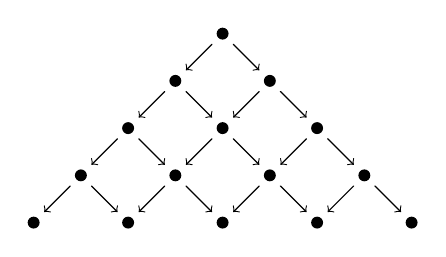
\begin{tikzpicture}[x=0.6cm,y=0.6cm,line cap=round]
		\fill (0,0) circle (0.5ex) coordinate (00);
		\fill (2,0) circle (0.5ex) coordinate (01);
		\fill (4,0) circle (0.5ex) coordinate (02);
		\fill (6,0) circle (0.5ex) coordinate (03);
		\fill (8,0) circle (0.5ex) coordinate (04);
		\fill (1,1) circle (0.5ex) coordinate (10);
		\fill (3,1) circle (0.5ex) coordinate (11);
		\fill (5,1) circle (0.5ex) coordinate (12);
		\fill (7,1) circle (0.5ex) coordinate (13);
		\fill (2,2) circle (0.5ex) coordinate (20);
		\fill (4,2) circle (0.5ex) coordinate (21);
		\fill (6,2) circle (0.5ex) coordinate (22);
		\fill (3,3) circle (0.5ex) coordinate (30);
		\fill (5,3) circle (0.5ex) coordinate (31);
		\fill (4,4) circle (0.5ex) coordinate (40);
		\draw[to-,shorten <=1.25ex,shorten >=1.25ex] (00) -- (10);
		\draw[to-,shorten <=1.25ex,shorten >=1.25ex] (01) -- (10);
		\draw[to-,shorten <=1.25ex,shorten >=1.25ex] (01) -- (11);
		\draw[to-,shorten <=1.25ex,shorten >=1.25ex] (02) -- (11);
		\draw[to-,shorten <=1.25ex,shorten >=1.25ex] (02) -- (12);
		\draw[to-,shorten <=1.25ex,shorten >=1.25ex] (03) -- (12);
		\draw[to-,shorten <=1.25ex,shorten >=1.25ex] (04) -- (13);
		\draw[to-,shorten <=1.25ex,shorten >=1.25ex] (10) -- (20);
		\draw[to-,shorten <=1.25ex,shorten >=1.25ex] (11) -- (20);
		\draw[to-,shorten <=1.25ex,shorten >=1.25ex] (11) -- (21);
		\draw[to-,shorten <=1.25ex,shorten >=1.25ex] (13) -- (22);
		\draw[to-,shorten <=1.25ex,shorten >=1.25ex] (12) -- (21);
		\draw[to-,shorten <=1.25ex,shorten >=1.25ex] (30) -- (40);
		\draw[to-,shorten <=1.25ex,shorten >=1.25ex] (31) -- (40);
		\draw[to-,shorten <=1.25ex,shorten >=1.25ex] (03) -- (13);
		\draw[to-,shorten <=1.25ex,shorten >=1.25ex] (12) -- (22);
		\draw[to-,shorten <=1.25ex,shorten >=1.25ex]  (21) -- (31);
		\draw[to-,shorten <=1.25ex,shorten >=1.25ex]  (22) -- (31);
		\draw[to-,shorten <=1.25ex,shorten >=1.25ex]  (20) -- (30);
		\draw[to-,shorten <=1.25ex,shorten >=1.25ex] (21) -- (30);
		\node[rotate=-45] at (2,1) {\pullbacksign};
		\node[rotate=-45] at (4,1) {\pullbacksign};
		\node[rotate=-45] at (6,1) {\pullbacksign};
		\node[rotate=-45] at (3,2) {\pullbacksign};
		\node[rotate=-45] at (5,2) {\pullbacksign};
		\node[rotate=-45] at (4,3) {\pullbacksign};
	\end{tikzpicture}
\end{center}
in $\Cc$ (shown here for $n=3$), and to be in $Q_n(\Cc)$ we require that all squares are pullbacks as indicated. Note that then in fact all rectangles you can find in this picture must be pullbacks.

The $Q_n(\Cc)$ assemble into a simplicial $\infty$-category $Q(\Cc)\colon \IDelta^\op\morphism \Cat_\infty$. To see this, one first shows that $\Fun(\TwAr([-])^\op,\Cc)\colon \IDelta^\op\morphism \Cat_\infty$ gives a functor. It's clear that all its ingredients are functorial, except perhaps for $\TwAr(-)$. But $\TwAr(-)\colon \sSet\morphism \sSet$ is right-adjoint to $(-)^\op\star (-)\colon \sSet\morphism \sSet$ (indeed, this guy has a right adjoint by \cref{thm:2Yoneda}, now unravel that $\TwAr(-)$ as defined in \cref{par:HomC}\itememph{b} fits the general description of such right adjoints), which one can show is a left Quillen functor for the Joyal model structure (by \cite[Proposition~D.5]{HigherCatsII} for example).

Now that we know $\Fun(\TwAr([-])^\op,\Cc)\colon \IDelta^\op\morphism \Cat_\infty$ is a functor, we only need to check that all the boundary and degeneracy maps preserve the full subcategories $Q_n(\Cc)$ described above. We leave this as an exercise. As you might have guessed, assigning to $\Cc$ the simplicial $\infty$-category $Q(\Cc)$ is called the \emph{Quillen $Q$-construction}.
\begin{propdef}\upshape\lecture[A sleep-deprived Fabian proves that $Q(\Cc)$ is a Segal $\infty$-category and introduces cartesian monoids.]{2020-11-24}\label{propdef:SpanQ}\itshape
	Let $\Cc$ be an $\infty$-category with pullbacks. The simplicial anima
	\begin{equation*}
		\core Q(\Cc)\colon \IDelta^\op\morphism \An
	\end{equation*}
	is a complete Segal space. Its associated category $\Span(\Cc)\simeq \asscat(\core Q(\Cc))$ is called the \emph{$\infty$-category of spans in $\Cc$}.
\end{propdef}
\begin{proof}
	We will actually prove that $Q(\Cc)$ itself satisfies the Segal and completeness conditions for simplicial $\infty$-categories rather than anima (really what this says is that there's an \emph{$\infty$-double category} $\Span^{(2)}(\Cc)$, but never mind that). Then all assertions for $\core Q(\Cc)$ will follow from the fact that $\core\colon \Cat_\infty\morphism\An$ preserves limits as it is a right-adjoint.
	
	Recall that the $0$-simplices in $\TwAr([n])^\op$ are given by morphisms in the poset $[n]$, i.e.\ by relations $(i\leq j)$. Now let $J_n\subseteq \TwAr([n])^\op$ be the subposet spanned by all $0$-simplices $(i\leq j)$ with $j\leq i+1$. In pictures, $J_n$ (for $n=3$) looks as follows:
	\begin{center}
		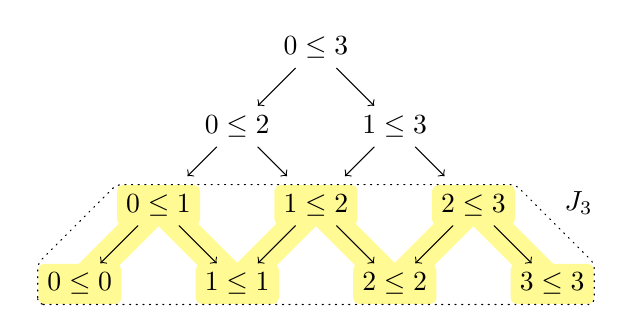
\begin{tikzpicture}[x=1cm,y=1cm,line cap=round, line join=round]
			\draw[line width=2.5ex,yellow!42!white] (0,0) to (1,1) to (2,0) to (3,1) to (4,0) to (5,1) to (6,0);
			\node[fill=yellow!42!white,rounded corners=2] (00) at (0,0) {$0\leq 0$};
			\node[fill=yellow!42!white,rounded corners=2] (01) at (2,0) {$1\leq 1$};
			\node[fill=yellow!42!white,rounded corners=2] (02) at (4,0) {$2\leq 2$};
			\node[fill=yellow!42!white,rounded corners=2] (03) at (6,0) {$3\leq 3$};
			\node[fill=yellow!42!white,rounded corners=2] (10) at (1,1) {$0\leq 1$};
			\node[fill=yellow!42!white,rounded corners=2] (11) at (3,1) {$1\leq 2$};
			\node[fill=yellow!42!white,rounded corners=2] (12) at (5,1) {$2\leq 3$};
			\node (20) at (2,2) {$0\leq 2$};
			\node (21) at (4,2) {$1\leq 3$};
			\node (30) at (3,3) {$0\leq 3$};
			\draw[to-] (00) -- (10);
			\draw[to-] (01) -- (10);
			\draw[to-] (01) -- (11);
			\draw[to-] (02) -- (11);
			\draw[to-] (02) -- (12);
			\draw[to-] (03) -- (12);
			\draw[to-,shorten <=1ex] (10) -- (20);
			\draw[to-,shorten <=1ex] (11) -- (20);
			\draw[to-,shorten <=1ex] (11) -- (21);
			\draw[to-,shorten <=1ex] (12) -- (21);
			\draw[to-]  (20) -- (30);
			\draw[to-] (21) -- (30);
			%\path (03.north east) to node {$J_3$} (12.north east);
			\draw[dotted,rounded corners=2] (00.south west) to (03.south east) to (03.north east) to node[above right] {$J_3$} (12.north east) to (10.north west) to node[above left] {$\phantom{J_n}$} (00.north west) to cycle;
		\end{tikzpicture}
	\end{center}
	Then one checks from the pointwise formula for Kan extensions (\cref{thm:KanExtension}) that a functor $F\colon \TwAr([n])^\op\morphism \Cc$ is in $Q_n(\Cc)$ iff it is right-Kan extended from $F|_{J_n}$. To see this in the example above, note that Kan extensions can be computed in steps (because right adjoints compose), so we may first Kan extend to the $0$-simplex $(0\leq 2)$, then to $(1\leq 3)$ and then finally to $(0\leq 3)$. In each step, the Kan extension is given by pullback, as one can see by restricting the limit from \cref{thm:KanExtension} to a suitable cofinal sub-$\infty$-category of the respective slice categories. The case for general $n$ works precisely the same. 
	
	In particular, since $J_n\subseteq \TwAr([n])^\op$ is fully faithful, we see that restriction to $J_n$ induces an equivalence
	\begin{equation*}
		Q_n(\Cc)\isomorphism \Fun(J_n,\Cc)
	\end{equation*}
	by \cref{cor:FullyFaithfulKanExtension}. The reason we don't work with the $J_n$ right away is that they do not form a cosimplicial $\infty$-category! So we have to include some redundant junk. However, the $J_n$ are closed under the maps induced by the Segal maps $e_i\colon [1]\morphism {[n]}$ (sending $[1]$ to $\{i,i+1\}\subseteq [n]$). These maps induce an equivalence $J_n\simeq J_1\sqcup_{J_0}\dotsb\sqcup_{J_0}J_1$ in $\Cat_\infty$, hence 
	\begin{align*}
		Q_n(\Cc)\simeq \Fun(J_1\sqcup_{J_0}\dotsb\sqcup_{J_0}J_1,\Cc)&\simeq \Fun(J_1,\Cc)\times_{\Fun(J_0,\Cc)}\dotsb\times_{\Fun(J_0,\Cc)}\Fun(J_1,\Cc)\\
		&\simeq Q_1(\Cc)\times_{Q_0(\Cc)}\dotsb\times_{Q_0(\Cc)}Q_1(\Cc)
	\end{align*}
	by \cref{cor:HomPreservesColimits}, which proves that $Q(\Cc)$ is indeed a Segal object in $\Cat_\infty$.
	
	For completeness, we have to check the condition from \cref{thmdef:RezkNerve}\itememph{b}, i.e.\ we need to show that
	\begin{equation*}
		\begin{tikzcd}[column sep=6em]
			Q_0(\Cc)\dar["s"']\rar["\Delta"]\drar[pullback]& Q_0(\Cc)\times Q_0(\Cc)\dar["{(s,s)}"]\\
			Q_3(\Cc)\rar["{\left(d_{\{0,2\}},d_{\{1,3\}}\right)}"]& Q_1(\Cc)\times Q_1(\Cc)
		\end{tikzcd}
	\end{equation*}
	is cartesian. So let $P$ be the pullback. We first check that the induced map $Q_0(\Cc)\morphism P$ is fully faithful. To see this, first note that the canonical map $\TwAr([n])^\op\morphism \TwAr([0])^\op$ induces a fully faithful map $s\colon \Fun(\TwAr([0])^\op,\Cc)\morphism\Fun(\TwAr([n])^\op,\Cc)$ for all $n$. Indeed, $\TwAr([0])^\op\simeq *$ is an anima, hence $s$ factors over the full subcategory $\Fun(|\TwAr([n])^\op|,\Cc)$. But $|\TwAr([n])^\op|\simeq *$ because $\TwAr([n])^\op$ contains $(0\leq n)$ as an initial element, and now it's clear that $s$ is indeed fully faithful. Hence so is $s\colon Q_0(\Cc)\morphism Q_n(\Cc)$ for all $n$.
	
	In particular, this is true for $n=3$. Moreover, $P\morphism Q_3(\Cc)$ is fully faithful too because it is a pullback of the fully faithful map $(s,s)\colon Q_0(\Cc)\times Q_0(\Cc)\morphism Q_1(\Cc)\times Q_1(\Cc)$. Now the diagram
	\begin{equation*}
		\begin{tikzcd}
			Q_0(\Cc)\rar\drar["s"',""{sloped,above,name=A}]& P\dar\\
			& Q_3(\Cc)\ar[from=A,to=1-2,phantom,pos=0.4,"\scriptscriptstyle/\!/\!/"]
		\end{tikzcd}
	\end{equation*}
	and the corresponding two-out-of-three property for fully faithful maps show that $Q_0(\Cc)\morphism P$ is fully faithful too.
	
	Now for essential surjectivity. The actual image of $Q_0(\Cc)\morphism P$ consists of the constant diagrams $F\colon \TwAr([3])^\op\morphism \Cc$, hence (by an easy argument) the essential image contains all diagrams that map all edges to equivalences. To see that every $0$-simplex in $P$ is a diagram $F\colon \TwAr([3])^\op\morphism \Cc$ of that form, we have to show the following:
	\begin{center}
		\begin{tikzpicture}[x=1.25cm,y=1.25cm,line cap=round]
			\node (00) at (0,0) {$F(0\leq 0)$};
			\node (01) at (2,0) {$F(1\leq 1)$};
			\node (02) at (4,0) {$F(2\leq 2)$};
			\node (03) at (6,0) {$F(3\leq 3)$};
			\node (10) at (1,1) {$F(0\leq 1)$};
			\node (11) at (3,1) {$F(1\leq 2)$};
			\node (12) at (5,1) {$F(2\leq 3)$};
			\node (20) at (2,2) {$F(0\leq 2)$};
			\node (21) at (4,2) {$F(1\leq 3)$};
			\node (30) at (3,3) {$F(0\leq 3)$};
			\draw[to-] (00) to  node[pos=0.5,above left=-0.6ex] {$\scriptscriptstyle(1)$} (10);
			\draw[to-] (01) to  node[pos=0.5,above right=-0.6ex] {$\scriptscriptstyle(2)$} (10);
			\draw[to-] (01) to  node[pos=0.5,below right=-0.6ex] {$\scriptscriptstyle(4)$} (11);
			\draw[to-] (02) to  node[pos=0.5,below left=-0.6ex] {$\scriptscriptstyle(4)$} (11);
			\draw[to-] (02) to  node[pos=0.5,above left=-0.6ex] {$\scriptscriptstyle(2)$} (12);
			\draw[to-] (03) to  node[pos=0.5,above right=-0.6ex] {$\scriptscriptstyle(1)$} (12);
			\draw[to-] (10) to  node[pos=0.5,above left=-0.6ex] {$\scriptscriptstyle(1)$}  (20);
			\draw[to-] (11) to  node[pos=0.7,below left=-0.6ex] {$\scriptscriptstyle(3)$} (20);
			\draw[to-] (11) to  node[pos=0.7,below right=-0.6ex] {$\scriptscriptstyle(3)$} (21);
			\draw[to-] (12) to  node[pos=0.5,above right=-0.6ex] {$\scriptscriptstyle(1)$} (21);
			\draw[to-]  (20) to  node[pos=0.5,above left=-0.6ex] {$\scriptscriptstyle(1)$}  (30);
			\draw[to-] (21) to  node[pos=0.5,above right=-0.6ex] {$\scriptscriptstyle(1)$}  (30);
			\draw[-to,dashed,bend right=35,FabiansPink] (30) to (10);
			\draw[-to,dashed,bend left=35,FabiansPink] (30) to (12);
			\draw[-to,dashed,bend right=35,FabiansPurple!67!FabiansPink] (20) to (00);
			\draw[-to,dashed,bend right=35,FabiansPurple!67!FabiansPink] (21) to (01);
			\draw[-to,dashed,bend left=35,FabiansPurple!67!FabiansPink] (20) to (02);
			\draw[-to,dashed,bend left=35,FabiansPurple!67!FabiansPink] (21) to (03);
			\node[rotate=-45] at (1.95,1.05) {\pullbacksign};
			\node[rotate=-45] at (4.05,1.05) {\pullbacksign};
			\node[rotate=-45] at (3,2.05) {\pullbacksign};
		\end{tikzpicture}
	\end{center}
	Suppose we are given a diagram $F\colon \TwAr([3])^\op\morphism \Cc$ in which all squares are pullbacks as indicated and such that the four dashed purple arrows are equivalences. Then all arrows are equivalences.
	
	Indeed, then the two dashed pink arrows $F(0\leq 3)\morphism F(0\leq 1)$ and $F(0\leq 3)\morphism F(2\leq 3)$ are equivalences as well, since they are pullbacks the purple arrows. By two-out-of-six, we see that all arrows labelled \enquote{$(1)$} must be equivalences.
	
	Now the commutative square
	\begin{equation*}
		\begin{tikzcd}
			F(0\leq 3)\rar[iso]\dar[iso]\drar[phantom,"\scriptscriptstyle/\!/\!/"] & F(1\leq 3)\dar[iso]\\
			F(0\leq 1)\rar & F(1\leq 1)
		\end{tikzcd}
	\end{equation*}
	shows that $F(0\leq 1)\morphism F(1\leq 1)$ is an equivalence. An analogous argument applies to $F(2\leq 3)\morphism F(2\leq 2)$. In other words, the two arrows labelled \enquote{$(2)$} are equivalences. This implies that the two arrows labelled \enquote{$(3)$} are equivalences, since they are pullbacks of the former. Finally, the two remaining arrows, labelled \enquote{$(4)$}, must be equivalences by two-out-of-three. We are done.
\end{proof}
	\renewcommand{\thechapter}{\Roman{chapter}}

\numpar*{Examples}\enquote{My first derived localizations}:
\begin{alphanumerate}
	\item If $W\subseteq R$ is a multiplicative subset in the commutative ring $R$, then $R\morphism R[W^{-1}]$ is a derived localization. This easily follows from \cref{propdef:derivedLocalization}\itememph{d} since $R[W^{-1}]$ is flat over $R$.
	\item For non-commutative rings, one needs the (left or right, who knows?) \emph{Ore condition} for $R\morphism R[W^{-1}]$ to be a derived localization.
	\item If $U\subseteq V$ is an open embedding of affine schemes, then $\Gamma(V,\Oo_V)\morphism\Global(U,\Oo_U)$ is a derived localization (but not necessarily an ordinary localization). Indeed, the condition from \cref{propdef:derivedLocalization}\itememph{d} easily shows that a ring morphism $\phi\colon R\morphism S$ is a derived localization iff $R_\pp\morphism S_\qq$ is a derived localization for all prime ideals $\qq\in \Spec S$ and $\pp\in \Spec R$ such that $\pp=\phi^{-1}(\qq)$. In our case of $\Gamma(V,\Oo_V)\morphism\Global(U,\Oo_U)$, all $\Oo_{V,v}\isomorphism \Oo_{U,v}$ for $v\in V$ are isomorphisms, hence they derived localizations for obvious reasons.
\end{alphanumerate}%\lecture[Wtf]{2020-11-19}
We will later see that $K$-theory has exact sequences for derived localizations!
\begin{proof}[Proof of \cref{propdef:derivedLocalization}]
	We already know \itememph{a} $\Leftrightarrow$ \itememph{b} $\Leftrightarrow$ \itememph{c} from \cref{propdef:BousfieldLocalization} and its dual. For \itememph{d} $\Leftrightarrow$ \itememph{e}, first note that $S\otimes_R^LR\isomorphism S$ is an equivalence. Indeed, we have
	\begin{equation*}
		H_i(S\otimes_R^LR)=\Tor_i^R(S,R)=\begin{cases*}
			S & if $i=0$\\
			0 & if $i\geq 1$
		\end{cases*}\,.
	\end{equation*}
	Now $S\otimes_R^L-$, being a left adjoint, commutes with colimits, which implies that
	\begin{equation*}
		\begin{tikzcd}
			S\rar["S\otimes_R^L\phi"]\dar\drar[pushout] & S\otimes_R^LS\dar\\
			0\rar & S\otimes_R^L(S/^LR)
		\end{tikzcd}
	\end{equation*}
	is a pullback square. This immediately implies $S\otimes_R^LS\simeq S$ iff $S\otimes_R^L(S/^LR)\simeq 0$, as desired.
	
	We finish the proof by showing \itememph{b} $\Leftrightarrow$ \itememph{d}. We must show that the counit $S\otimes_R^LC\morphism C$ is an equivalence for all $C\in \Dd(S)$ iff it is an equivalence for $S$. The \enquote{only if} direction being obvious, let's assume it is an equivalence for $S$. Then it is also an equivalence for all shifts $S[i]$. But the $\{S[i]\}_{i\in \IZ}$ generate $\Dd(S)$ under colimits and $S\otimes_R^L-$ commutes with colimits, so we are done.
\end{proof}

\lecture[The Rezk nerve and (complete) Segal spaces/anima.\newline --- \enquote{\emph{Today is brainf*ck time. There's no deep content, except for the things I'm not saying.}}]{2020-11-19}Today we get back to the Rezk-nerve. Recall the functor $\N^r\colon \Cat_\infty\morphism \cat{s}\An$ introduced in \cref{exm:RezkNerve}\itememph{b}.
\begin{thmdef}[Rezk, Joyal--Tierney, Lurie]\label{thmdef:RezkNerve}
	The Rezk nerve functor $\N^r\colon \Cat_\infty\morphism \cat{s}\An$ is fully faithful and its essential image consists of the complete Segal spaces/anima. Here a \emph{Segal anima} is a cosimplicial anima $X\colon \IDelta^\op\morphism \An$ such that
	\begin{equation*}
		X_n\simeq \Hom_{\cat{s}\An}(\Delta^n,X)\isomorphism \Hom_{\cat{s}\An}(I_n,X)\simeq X\times_{X_0}X_1\times_{X_0}\dotsb\times_{X_0}X_1
	\end{equation*}
	is an equivalence for all $n$ \embrace{as usual $I_n$ denotes the $n$-spine, which is an iterated pushout of copies of $\Delta^1$, hence the pullback on the right-hand side}. We call $X$ \emph{complete} if the following equivalent conditions hold:
	\begin{alphanumerate}
		\item Also the restriction $X_0\simeq \Hom_{\cat{s}\An}(\Delta^0,X)\isomorphism \Hom_{\cat{s}\An}(J,X)$ along $J\morphism \Delta^0$ is an equivalence, where $J$ is the \embrace{ordinary nerve of the} free-living isomorphism.
		\item The diagram
		\begin{equation*}
			\begin{tikzcd}[column sep=5em]
				X_0\dar["s"']\rar["\Delta"]\drar[pullback] & X_0\times X_0\dar["{(s,s)}"]\\
				X_3\rar["{(d_{\{0,2\}},d_{\{1,3\}})}"] & X_1\times X_1
			\end{tikzcd}
		\end{equation*}
		is cartesian \embrace{note that $\Delta$ denotes a good old diagonal and not some simplicial stuff}.
		\item The degeneracy map $s\colon X_0\isomorphism X_1^\times$ is an equivalence, where $X_1^\times\subseteq X_1$ is the collection of path components of those $g\in X_1$ for which the following holds: Let $x=d_1(g)$ and $y=d_0(g)$ and for arbitrary $w,z\in X_0$ put 
		\begin{equation*}
			\begin{tikzcd}
				P_{w,z}\rar\dar\drar[pullback]& X_1\dar["{(d_1,d_0)}"]\\
				\{(w,z)\}\rar& X_0\times X_0
			\end{tikzcd}
		\end{equation*}
		Moreover, there is a \enquote{composition map}
		\begin{equation*}
			\begin{tikzcd}[column sep=2.7em]
				\operatorname{comp}\colon X_1\times_{d_1,X_0,d_0}X_1 & X_2\morphism[d_1]X_1\lar["{(d_0,d_1)}"',"\sim"]
			\end{tikzcd}
		\end{equation*}
		which, after restriction to $P_{w,x}\simeq P_{w,x}\times_{\{x\}}\{g\}$ and $P_{y,z}\simeq \{g\}\times_{\{y\}}P_{y,z}$ induces \enquote{post- and precomposition maps}
		\begin{equation*}
			g_*\colon P_{w,x}\morphism P_{w,y}\quad\text{and}\quad g^*\colon P_{y,z}\morphism P_{x,z}\,.
		\end{equation*}
		Then we put $x\in X_1^\times$ iff $g_*$ and $g^*$ are equivalences for all $w,z\in X_0$.
		\item The simplicial subanima $X^\times$ given by 
		\begin{equation*}
			[n]\longmapsto X_n^\times\coloneqq\left\{\begin{tabular}{c}
				collection of path components in\\
				$X_n$ such that all edges lie in $X_1^\times$
			\end{tabular}\right\}
		\end{equation*}
		is constant. Note that $X_0^\times=X_0$, so it is actually constant on $X_0$.
 	\end{alphanumerate}
\end{thmdef}
To understand these conditions a bit better, Fabian drew the following picture for \cref{thmdef:RezkNerve}\itememph{b}:
\begin{center}
	\begin{tikzpicture}[line cap=round, line join=round,decoration={markings,mark=at position 0.5 with {\arrow{to}}},x=0.75cm,y=0.75cm]
		\coordinate (0) at (-1.75,-0.3);
		\node[left] at (0) {$0$};
		\coordinate (1) at (-0.25,1);
		\node[above] at (1) {$1$};
		\coordinate (2) at (0,-1);
		\node[below] at (2) {$2$};
		\coordinate (3) at (1.25,0);
		\node[right] at (3) {$3$};
		\draw[postaction={decorate}](0) to (1);
		\draw[postaction={decorate},line width=0.8] (0) to node[pos=0.5,below left] {$\scriptstyle\id$} (2);
		\draw[postaction={decorate}] (1) to (2);
		\draw[postaction={decorate}] (2) to (3);
		\draw[postaction={decorate},line width=0.8] (1) to node[pos=0.5,above right] {$\scriptstyle\id$} (3);
		\draw[dashed,postaction={decorate}] (0) to (3);
	\end{tikzpicture}
\end{center}
So what condition~\itememph{b} is trying to say is that whenever a $3$-simplex $\Delta^3$ in $X_3$ has degenerate $\Delta^{\{0,2\}}$- and $\Delta^{\{1,3\}}$-edges, then all its edges are degenerate and the $3$-simplex itself is equivalent to a degenerate one. To get a grasp on condition~\itememph{d}, note that for any $\infty$-category $\Cc$ we have $\core\Cc$ encoded in $\N^r(\Cc)$ in two different ways: First in a direct fashion, as $\core\Cc\simeq \Hom_{\Cat_\infty}([0],\Cc)\simeq \N_0^r(\Cc)$, and second as the full subanima of $\core\Ar(\Cc)\simeq \N_1^r(\Cc)$ spanned by the equivalences in $\Cc$ (essentially because $\Delta^1\morphism \Delta^0$ is a localization). So $\N^r(\Cc)^\times$ should be constant with value $\core \Cc$.

\begin{proof}[Not a proof of \cref{thmdef:RezkNerve}]
	The proof is difficult, mostly the first statement that $\N^r$ is fully faithful. The original proof of Joyal--Tierney can be found in \cite{JoyalTierney} and Lurie's poof is in \cite{LurieGoodwillieCalculus}. However, Fabian recommends to prove the equivalence of the four conditions as a (not easy, but doable) exercise, as well as to prove that $\N^r(\Cc)$ is a complete Segal space for all $\infty$-categories $\Cc$.
	
	The key step to prove that $\N^r$ is fully faithful is to give a description of $\asscat(X)$ for $X$ a (not necessarily complete) Segal space: There is a canonical equivalence
	\begin{equation}\label{eq:asscat1}
		\core\asscat(X)\simeq |X^\times|\,,
	\end{equation}
	where $|\blank|\colon \cat{s}\An\morphism \An$ denotes the colimit functor over $\IDelta^\op$.
	\begin{urem}
		Note that the notation $|\blank|\simeq \colimit_{\IDelta^\op}$ is consistent with our notation for the geometric realization of simplicial sets: If $T\colon \IDelta^\op\morphism \Set\subseteq \An$ is a simplicial set/discrete simplicial anima, then the homotopy colimit of $T$ is weakly homotopy equivalent to $T$, so
		\begin{equation*}
			\colimit_{\IDelta^\op}T\simeq \Big(\hocolimit_{\CC[\IDelta^\op]}T\Big)^\mathrm{f}\simeq T^\mathrm{f}\simeq \Sing|T|
		\end{equation*}
		using \cref{thm:HomotopyLimits}. The notation is also consistent with $|\blank|\colon\Cat_\infty\morphism \An$ in that generally for a simplicial anima $T\colon \IDelta^\op\morphism\An$ we have
		\begin{equation*}
			|\asscat(T)|\simeq |T|\,.
		\end{equation*}
		Indeed, this follows from \cref{thm:ColimitPreservingRepresentable} as both sides are colimit-preserving functors that send $[n]\mapsto *\in \An$ for all $n\in \IN$. Here and in the following, $[n]$ always denotes the $\infty$-category associated to this poset, and $\Delta^n\in \sSet\subseteq\cat{s}\An$ always denotes the discrete (but not constant) simplicial anima.
	\end{urem}
	Moreover, one can show that for every (not necessarily complete) Segal space $X$ there are pullback diagrams
	\begin{equation}\label{eq:asscat2}
		\begin{tikzcd}
			\Hom_{\asscat(X)}(x,y)\dar\rar\drar[pullback] & X_1\dar["{(d_1,d_0)}"]\\
			\{(x,y)\}\rar & X_0\times X_0
		\end{tikzcd}
	\end{equation}
	for all $x,y\in X_0$ (in particular $\Hom_{\asscat(X)}(x,y)\simeq P_{x,y}$ in the notation of \itememph{b}). This will become important later.
	
	With \cref{eq:asscat1} and \cref{eq:asscat2}, the proof of \cref{thmdef:RezkNerve} becomes quite easy. To prove that $\N^r$ is fully faithful, we must show that the counit $\asscat(\N^r(\Cc))\isomorphism \Cc$ is an equivalence for all $\Cc\in \Cat_\infty$. It is an equivalence on cores because
	\begin{equation*}
		\core\asscat\big(\N^r(\Cc)\big)\simeq |\N^r(\Cc)^\times|\quad\text{and}\quad \core\Cc\simeq \N_0^r(\Cc)\,;
	\end{equation*}
	since $\N^r(\Cc)$ is complete, $\N^r(\Cc)^\times$ is constant on $\N_0^r(\Cc)$, hence the colimit over $\IDelta^\op$ (recall $|\IDelta^\op|\simeq *$) is just $|\N^r(\Cc)^\times|\simeq \N_0^r(\Cc)$, as claimed. This shows that the counit is essentially surjective.
	
	To prove that it is fully faithful, i.e.\ induces equivalences on $\Hom$ anima, observe that using \cref{eq:asscat2} it induces the following equivalence of pullback squares:
	\begin{equation*}
		\begin{tikzcd}[column sep=tiny, row sep=small]
			\Hom_{\asscat(\N^r(\Cc))}(x,y)\ar[rr] \ar[dd]\ar[dddr,pullback]\drar& & \Hom_\Cc(x,y)\ar[dd]\drar\ar[dddr,pullback]\\
			& \N_1^r(\Cc)\ar[rr,iso,pos=0.4,crossing over] & & \core\Ar(\Cc)\ar[dd]\\
			\{(x,y)\}\drar\eqar[rr] & & \{(x,y)\}\drar\\
			& \N_0^r(\Cc)\times\N_0^r(\Cc)\ar[<-,uu,crossing over]\ar[rr,iso] & & \core\Cc\times\core\Cc
		\end{tikzcd}
	\end{equation*}
	For the right pullback square, recall that a pullback of $\infty$-categories with one leg an inner fibration induces a pullback on cores, hence the usual pullback diagram for $\Hom_\Cc(x,y)$ passes to cores. This finishes the \dotso well, not \emph{proof}, but whatever else this is.
\end{proof}
The composite functor
\begin{equation*}
	\cat{s}\An\xrightarrow{\asscat}\Cat_\infty\morphism[\N^r]\cat{s}\An
\end{equation*}
is called \emph{completion}. Unwinding definitions, one finds that it is a left-adjoint to the inclusion $\{\text{complete Segal spaces}\}\subseteq \cat{s}\An$. Fabian remarks that the completion functor is impossible to control outside of Segal spaces.
\begin{exm}\label{exm:MyFirstRezkNerves}
	\enquote{My first Rezk nerves}:
	\begin{alphanumerate}
		\item The ordinary nerve $\N(\Cc)\in \sSet\subseteq\cat{s}\An$ of a $1$-category is a Segal \emph{set} and thus also a Segal anima since $\Set\subseteq \An$ preserves limits. But it is usually not complete! In fact, we have
		\begin{equation*}
			\begin{tikzcd}
				\N_0(\Cc)\dar["s"']\eqar[r]&\left\{\text{set of objects in $\Cc$}\right\}\dar\\
				\N_1(\Cc)\eqar[r]&\left\{\text{set of isomorphisms in $\Cc$}\right\}
			\end{tikzcd}
		\end{equation*}
		where the right vertical arrow takes $x\in \Cc$ to $\id_x$. But usually, there are more isomorphisms in a category than just the identities, hence $\N_1(\Cc)^\times$ is usually larger than $\N(\Cc)_0$.
		\item The two functors
		\begin{equation*}
			\begin{gathered}\nonumber
				\cat{s}\An\xrightarrow{\asscat} \Cat_\infty \morphism[\pi]\Cat_1^{(2)}\\
				\cat{s}\An\xrightarrow{\cat{s}\pi_0}\sSet\morphism[h]\Cat_1
			\end{gathered}
		\end{equation*}
		are different, even though both are colimit-preserving and take $\Delta^n\mapsto [n]$. The reason is of course that $\Cat_1\subseteq \Cat_1^{(2)}$ doesn't preserve colimits. To obtain explicit counterexamples, you can take $\const S^1$ or $\N^r(\{\text{finite-dimensional vector spaces}\})$ for example.
		
		Both functors do, however, agree on ordinary nerves $\N(\Cc)$ of $1$-categories. Nevertheless, Fabian warns you to never look at the lower functor.
		\item The adjunction $\asscat\colon \cat{s}\An\shortdoublelrmorphism\Cat_\infty\noloc \N^r$ restricts to an equivalence
		\begin{equation*}
			\ev_0\colon\{\text{constant simplicial anima}\}\doublelrmorphism[\sim][\sim]\An\noloc \const\,.
		\end{equation*}
		Indeed, $\N_n^r(K)\simeq \core\Fun([n],K)\simeq \Fun(|[n]|,K)\simeq K$ as $|[n]|\simeq *$.
		\item A more nontrivial example is that
		\begin{equation*}
			\N_n^r\big(\TwAr(\Cc)\big)\simeq \Hom_{\Cat_\infty}\big([n]^\op\star[n],\Cc\big)\simeq \Hom_{\cat{s}\An}\big((\Delta^n)^\op\star\Delta^n,\N^r(\Cc)\big)\,.
		\end{equation*}
		To prove this, recall from \cref{par:MoreOnTwAr} that there is a pullback square
		\begin{equation*}
			\begin{tikzcd}
				\TwAr(\Cc)\dar\rar\drar[pullback]& */\An\dar\\
				\Cc^\op\times\Cc\rar["\Hom_\Cc"]& \An
			\end{tikzcd}
		\end{equation*}
		(depending on your definitions, this is a pullback both in simplicial sets and in $\Cat_\infty$ or only in $\Cat_\infty$). Now we do a computation in several steps, each of which will be justified below:\newcounter{foo}
		\begin{align}
			\N_n^r\big(\TwAr(\Cc)\big)&\mathrel{\overset{\phantom{2}}{\simeq}}\Hom_{\Cat_\infty}\big([n],\TwAr(\Cc)\big)\nonumber\\
			&\mathrel{\overset{(1)}{\simeq}}\Hom_{\Cat_\infty}\big([n],\Cc^\op\times\Cc\big)\times_{\Hom_{\Cat_\infty}([n],\An)}\Hom_{\Cat_\infty}\big([n],*/\An\big)\label{eq:Umformung1}\tag*{}\\
			&\mathrel{\overset{(2)}{\simeq}}\Hom_{\Cat_\infty}\big([n],\Cc^\op\times\Cc\big)\times_{\core(\Cc^\op\times\Cc)}\core\big((\Cc^\op\times\Cc)\times_{\An}*/\An\big)\label{eq:Umformung2}\tag*{}\\\refstepcounter{foo}
			&\mathrel{\overset{(3)}{\simeq}}\big(\Hom_{\Cat_\infty}\big([n]^\op,\Cc\big)\times\Hom_{\Cat_\infty}\big([n],\Cc\big)\big)\times_{\core(\Cc^\op\times\Cc)}\core\TwAr(\Cc)\label{eq:Umformung3}\tag*{}\\
			&\mathrel{\overset{(4)}{\simeq}}\big(\Hom_{\Cat_\infty}\big([n]^\op,\Cc\big)\times\Hom_{\Cat_\infty}\big([n],\Cc\big)\big)\times_{\core(\Cc\times\Cc)}\core\Ar(\Cc)\label{eq:Umformung4}\tag*{}\\
			&\mathrel{\overset{(5)}{\simeq}}\core\Fun\big([n]^\op\sqcup_{\{0\}}[1]\sqcup_{\{0\}}[n],\Cc\big)\label{eq:Umformung5}\tag*{}\\
			&\mathrel{\overset{(6)}{\simeq}}\Hom_{\Cat_\infty}\big([n]^\op\star[n],\Cc\big)\label{eq:Umformung6}\tag*{}\\
			&\mathrel{\overset{(7)}{\simeq}} \Hom_{\cat{s}\An}\big((\Delta^n)^\op\star\Delta^n,\N^r(\Cc)\big)\label{eq:Umformung7}\tag*{}
		\end{align}
		Step~\hyperref[eq:Umformung1]{(1)} follows from the pullback square above via the dual of \cref{cor:HomPreservesColimits}. Next we discuss step~\hyperref[eq:Umformung2]{(2)}, which will need by far the most justification of them all: First, the map $\Hom_{\Cat_\infty}([n],\Cc^\op\times\Cc)\morphism \Hom_{\Cat_\infty}({0},\Cc^\op\times\Cc)\simeq\core(\Cc^\op\times \Cc)$ that is implicit in the pullback is induced by restriction along $\{0\}\monomorphism {[n]}$, i.e.\ \enquote{evaluation at $0$}. Now there is a pullback square
		\begin{equation*}
			\begin{tikzcd}
				\Hom_{\Cat_\infty}\big([n],*/\An\big)\rar["\ev_0"]\dar\drar[pullback]&*/\An\dar\\
				\Hom_{\Cat_\infty}\big([n],\An\big)\rar["\ev_0"] & \An
			\end{tikzcd}
		\end{equation*}
		in $\An$. To see this, note that $\Fun([n],*/\An)\simeq \Fun^*([n+1],\An)$ holds by the join-slice adjunction (or by inspection), where $\Fun^*$ denotes the full sub-$\infty$-categories of functors taking $0\mapsto *\in \An$.
		Similarly $*/\An\simeq \Fun^*([1],\An)$. Now $[n+1]$ can be written as a pushout 
		$[1]\sqcup_{\{1\}}\{1,\dotsc,n\}$ (if you take the pushout in $\sSet$, then $\Delta^1\sqcup_{\{1\}}\Delta^{\{1,\dotsc,n\}}\monomorphism \Delta^n$ will be inner anodyne, hence $[n+1]$ is the correct pushout in $\Cat_\infty$ by \cref{thm:HomotopyLimits}) and the above pullback square follows from \cref{cor:HomPreservesColimits}. Now plugging this pullback into \hyperref[eq:Umformung1]{(1)} gives \hyperref[eq:Umformung2]{(2)} after some abstract nonsense pullback manipulations.
		
		For~\hyperref[eq:Umformung3]{(3)} note that $\Hom_{\Cat_\infty}([n],\Cc^\op\times\Cc)\simeq \Hom_{\Cat_\infty}([n],\Cc^\op)\times\Hom_{\Cat_\infty}([n],\Cc)$ and we have $\Fun([n],\Cc^\op)\simeq \core\Fun([n]^\op,\Cc)^\op$. But the $(-)^\op$ vanishes upon taking cores, hence $\Hom_{\Cat_\infty}([n],\Cc^\op)\simeq \Hom_{\Cat_\infty}([n]^\op,\Cc)$. This explains the left factor in the pullback. For the right factor, use that $\core$, being a right-adjoint functor, commutes with pullbacks.
		
		Step~\hyperref[eq:Umformung4]{(4)} follows straight from \cref{exc:coreTwAr=coreAr}. Step~\hyperref[eq:Umformung5]{(5)} is immediate from \cref{cor:HomPreservesColimits} and for \hyperref[eq:Umformung6]{(6)} we need to check that the pushout in question, when taken in $\Cat_\infty$, is given by $[n]^\op\star[n]$. This can be done as before: Take the pushout in $\sSet$ and verify that the canonical map to $[n]^\op\star[n]$ is inner anodyne.
		
		Finally, \hyperref[eq:Umformung7]{(7)} is immediate once we convinced ourselves that
		\begin{equation*}
			\N^r([n]^\op\star [n])\simeq (\Delta^n)^\op\star\Delta^n\,,
		\end{equation*}
		since $\N^r$ is fully faithful by \cref{thmdef:RezkNerve}. To obtain the equation above, note that $\Hom_{\Cat_\infty}([m],[n]^\op\star [n])\simeq \Hom_{\Cat_1}([m],[n]^\op\star [n])$ (where we view the right-hand as a discrete anima), since all $\infty$-categories involved here are actually nerves of $1$-categories (although we always surpress the nerve in our notation).
		\item As a final example, let's define \emph{span categories}: Let $\Cc$ be an $\infty$-category and let $Q_n(\Cc)\subseteq \Fun(\TwAr(\Delta^n)^\op,\Cc)$ be the full sub-$\infty$-category consisting of those functors that take all \enquote{squares} in $\TwAr(\Delta^n)^\op$ to pullbacks. To make sense of this, recall our description of $\TwAr(\Delta^n)$ from \cref{par:MoreOnTwAr}. In that way, a functor $\TwAr(\Delta^n)^\op\morphism \Cc$ can be pictured as a diagram
		\begin{center}
			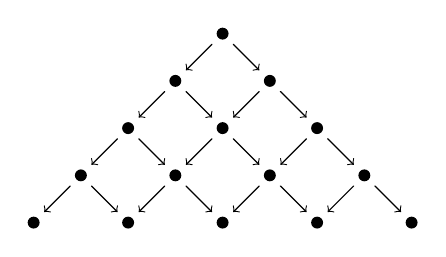
\begin{tikzpicture}[x=0.6cm,y=0.6cm,line cap=round]
				\fill (0,0) circle (0.5ex) coordinate (00);
				\fill (2,0) circle (0.5ex) coordinate (01);
				\fill (4,0) circle (0.5ex) coordinate (02);
				\fill (6,0) circle (0.5ex) coordinate (03);
				\fill (8,0) circle (0.5ex) coordinate (04);
				\fill (1,1) circle (0.5ex) coordinate (10);
				\fill (3,1) circle (0.5ex) coordinate (11);
				\fill (5,1) circle (0.5ex) coordinate (12);
				\fill (7,1) circle (0.5ex) coordinate (13);
				\fill (2,2) circle (0.5ex) coordinate (20);
				\fill (4,2) circle (0.5ex) coordinate (21);
				\fill (6,2) circle (0.5ex) coordinate (22);
				\fill (3,3) circle (0.5ex) coordinate (30);
				\fill (5,3) circle (0.5ex) coordinate (31);
				\fill (4,4) circle (0.5ex) coordinate (40);
				\draw[to-,shorten <=1.25ex,shorten >=1.25ex] (00) -- (10);
				\draw[to-,shorten <=1.25ex,shorten >=1.25ex] (01) -- (10);
				\draw[to-,shorten <=1.25ex,shorten >=1.25ex] (01) -- (11);
				\draw[to-,shorten <=1.25ex,shorten >=1.25ex] (02) -- (11);
				\draw[to-,shorten <=1.25ex,shorten >=1.25ex] (02) -- (12);
				\draw[to-,shorten <=1.25ex,shorten >=1.25ex] (03) -- (12);
				\draw[to-,shorten <=1.25ex,shorten >=1.25ex] (04) -- (13);
				\draw[to-,shorten <=1.25ex,shorten >=1.25ex] (10) -- (20);
				\draw[to-,shorten <=1.25ex,shorten >=1.25ex] (11) -- (20);
				\draw[to-,shorten <=1.25ex,shorten >=1.25ex] (11) -- (21);
				\draw[to-,shorten <=1.25ex,shorten >=1.25ex] (13) -- (22);
				\draw[to-,shorten <=1.25ex,shorten >=1.25ex] (12) -- (21);
				\draw[to-,shorten <=1.25ex,shorten >=1.25ex] (30) -- (40);
				\draw[to-,shorten <=1.25ex,shorten >=1.25ex] (31) -- (40);
				\draw[to-,shorten <=1.25ex,shorten >=1.25ex] (03) -- (13);
				\draw[to-,shorten <=1.25ex,shorten >=1.25ex] (12) -- (22);
				\draw[to-,shorten <=1.25ex,shorten >=1.25ex]  (21) -- (31);
				\draw[to-,shorten <=1.25ex,shorten >=1.25ex]  (22) -- (31);
				\draw[to-,shorten <=1.25ex,shorten >=1.25ex]  (20) -- (30);
				\draw[to-,shorten <=1.25ex,shorten >=1.25ex] (21) -- (30);
				\node[rotate=-45] at (2,1) {\pullbacksign};
				\node[rotate=-45] at (4,1) {\pullbacksign};
				\node[rotate=-45] at (6,1) {\pullbacksign};
				\node[rotate=-45] at (3,2) {\pullbacksign};
				\node[rotate=-45] at (5,2) {\pullbacksign};
				\node[rotate=-45] at (4,3) {\pullbacksign};
			\end{tikzpicture}
		\end{center}
		in $\Cc$ (shown here for $n=3$), and to be in $Q_n(\Cc)$ we require that all squares are pullbacks as indicated. Note that then in fact all rectangles you can find in this picture must be pullbacks.
		
		The $Q_n(\Cc)$ assemble into a cosimplicial $\infty$-category $Q(\Cc)\colon \IDelta^\op\morphism \Cc$. This is, you might have guessed it, the \emph{Quillen $Q$-construction}. Also define the \emph{spam category} of $\Cc$ to be $\Span(\Cc)\simeq \asscat(\core Q(\Cc))$.
	\end{alphanumerate}
\end{exm}


\backmatter\KOMAoption{chapterprefix}{false}
\printbibliography
\end{document}